\documentclass[12pt,spanish,a4paper]{report}

\usepackage{amssymb}
\setcounter{tocdepth}{3}
\usepackage{url}
\usepackage[utf8x]{inputenc}
\usepackage[spanish]{babel}
\usepackage{graphicx}
\usepackage{hyperref}
\usepackage{listings}
\usepackage{appendix}
\usepackage{makeidx}
\usepackage{fancyhdr}
\usepackage{textcomp}
\usepackage{float}
\usepackage{amssymb, amsmath}
\usepackage{multicol}
\usepackage{anysize}
\usepackage{pdflscape}
\usepackage[usenames,dvipsnames]{color}
\usepackage[font=footnotesize,labelfont=bf]{caption}
\usepackage[T1]{fontenc}  % permite copiar correctamente el texto del pdf.

\hypersetup{
    bookmarks=true,         % show bookmarks bar?
    unicode=false,          % non-Latin characters in Acrobat’s bookmarks
    pdftoolbar=true,        % show Acrobat’s toolbar?
    pdfmenubar=true,        % show Acrobat’s menu?
    pdffitwindow=false,     % window fit to page when opened
    pdfstartview={FitH},    % fits the width of the page to the window
	pdfsubject={Proyecto Final de la carrera Lic. en Ciencias de la Computaci\'on - UNRC},   % subject of the document
    pdftitle={Implementaci\'on de una capa de distribuci\'on del framework FuD usando el middleware BOINC},    % title
    pdfauthor={Lucas Besso - Ra\'ul Striglio},     % author
    pdfproducer={http://www.fudepan.org.ar/}, % producer of the document
    pdfkeywords={fud} {fud-boinc} {fudepan} {boinc} {tesis} {unrc} {computacion voluntaria}, % list of keywords
    pdfnewwindow=false,      % links in new window
    colorlinks=true,       % false: boxed links; true: colored links
    linkcolor=Red,          % color of internal links
    citecolor=Green,        % color of links to bibliography
    filecolor=Magenta,      % color of file links
    urlcolor=Blue           % color of external links
}

\marginsize{3cm}{3cm}{3cm}{3cm}
\pagestyle{fancy}

\fancyhf{}
\fancyhead[R]{\bfseries\thepage}
\fancyhead[L]{\bfseries\rightmark}

\cfoot{\scriptsize Implementación de una capa de distribución del framework FuD usando el middleware BOINC }

%Commands
\newcommand{\HRule}{\rule{\linewidth}{0.5mm}}
\renewcommand\lstlistingname{Código}
\renewcommand\lstlistlistingname{Índice de códigos fuente}

\definecolor{gris}{RGB}{245, 245, 245}

%para evitar que corte las palabras
\pretolerance=3000
\tolerance=3000


% Fix the line-breaking
\sloppy


\begin{document}
	\pagenumbering{roman}

	\begin{titlepage} 
		\begin{center}
		
			%Escudos
            \begin{minipage}{0.45\textwidth}
                \begin{center}
                    %Escudo UNRC
                    
\includegraphics[width=60pt,height=90.5pt]{images/escudo.jpg}\\
                    \begin{footnotesize}
                        \textsc{Universidad Nacional de Río Cuarto} \\
                    \end{footnotesize}
                    \vfill
                    \begin{scriptsize}
                        \textsc{Fac. de Cs. Exactas, Fco-Qcas y Naturales} \\
                        \textsc{Departamento de Computación} \\[1cm]    
                    \end{scriptsize}
                \end{center}
            \end{minipage}
            \begin{minipage}{0.45\textwidth}
                \begin{center}
                    %Escudo FuDePAN
                    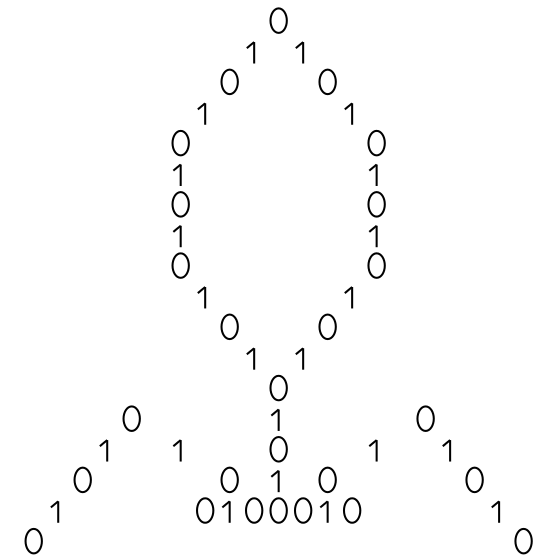
\includegraphics[width=90pt,height=90pt]{images/logo-fudepan.png}\\
                    \vfill
                    \begin{footnotesize}
                        \textsc{FuDePAN} \\
                    \end{footnotesize}
                    \begin{scriptsize}
                        \textsc{Fundación para el Desarrollo de la Programación en Ácidos Nucleicos} \\[1cm]    
                    \end{scriptsize}
                \end{center}
            \end{minipage}

			\textsc{\\[2cm] \large Trabajo Final}\\[0.2cm]
			\textsc{Licenciatura en Ciencias de la Computación}\\[0.2cm]

			\HRule
			{ \Large \bfseries Implementación de una capa de distribución \\del framework FuD usando el middleware \\BOINC\\}
			\HRule 
			\\[4cm]
			

			\begin{multicols}{3}
				\begin{center} \large
					\emph{Autores:}\\
					Lucas \textsc{Besso}\\
					Raúl \textsc{Striglio}
				\end{center}
				\columnbreak  
			
				\begin{center} \large
					\emph{Director:} \\
					Lic. Laura \textsc{Tardivo}
				\end{center}
				\columnbreak  
			
				\begin{center} \large
				\emph{Co-Director:} \\
				Daniel \textsc{Gutson}
				\end{center}
			\end{multicols}
			
			\vfill
			\today
			%{15 de diciembre de 2011}

		\end{center}
	\end{titlepage}

	\newpage

	%Resumen
	\begin{abstract}
El cómputo sobre grandes conjuntos de datos es un tema importante dentro de la ciencia de la computación. Mucha información es inherentemente difícil de comprimir y a su vez los recursos para procesar esta cantidad de datos usualmente son muy costosos. Las organizaciones sin fines de lucro, instituciones educacionales, etc. deben encontrar la manea de manejar sus requerimientos computacionales intentando mantener los costos lo más bajo posible. Existen varias herramientas que permiten solucionar este problema mediante alguna forma de computación distribuida.

Este trabajo brinda un panorama general sobre el diseño, implementación y pruebas de una nueva capa de distribución para el framework FuD con el objetivo de permitirle a éste hacer uso de la arquitectura BOINC para realizar computación voluntaria.

El enfoque elegido fue hacer uso de las librerías ofrecidas por BOINC para poder integrar sus funcionalidades como parte del comportamiento de la capa de distribución de FuD.
	\end{abstract}

	\chapter*{Agradecimientos}
\label{chapter:agradecimientos}
\addcontentsline{toc}{chapter}{Agradecimientos}

El trabajo aquí presentado es el fruto de toda una carrera de estudio y sacrificios. Durante este trayecto, un interminable número de personas ofrecieron de diversas maneras su granito de arena para apoyarnos y darnos las fuerzas necesarias para lograr nuestro objetivo, a pesar de los diferentes obstáculos que se presentan en la vida.

En primer lugar queremos agradecer especialmente a los directores de esta tesis: Daniel Gutson y Guillermo Biset, quienes fueron los pioneros y mentes extraordinarias de este proyecto. Ambos depositaron su voto de confianza en nosotros para que llevemos adelante este trabajo final, destinando parte de sus valiosos tiempos para ayudarnos y corregirnos en momentos cruciales.

También queremos darle nuestro inmenso agradecimiento a Laura Tardivo por aceptar ser nuestra directora y por la excelente disposición que tuvo al ayudarnos en la última etapa del proyecto.

No queremos dejar de nombrar a la gente de FuDePAN por su buena onda y predisposición para ayudar, especialmente Hugo Arregui quien ha colaborado activamente con nosotros en momentos críticos del proyecto.

En el plano personal, el primer agradecimiento va por supuesto a nuestras familias, a quienes les debemos todo lo que somos ya que sin ellos hoy no podríamos haber llegado hasta donde hemos llegado, sobre todo por el gran esfuerzo que han realizado a lo largo de todos estos años.

Un especial agradecimiento a nuestros amigos que siempre estuvieron presentes en las buenas y en las malas brindándonos todo su apoyo, a nuestra respectivas novias quienes tuvieron que soportar nuestras locuras demostrándonos su cariño y apoyo incondicional.

Tampoco queremos olvidarnos de todos los profesores amigos que hemos conocido durante estos años de estudio brindándonos todo su potencial educativo para que podamos salir adelante.

A todas estas personas les queremos enviar nuestros más profundos \linebreak agradecimientos.


	
	\tableofcontents
	\listoffigures 
	\lstlistoflistings
    \listoftables
	
	\newpage
	\pagenumbering{arabic}
	
	\part{Preliminar}\label{prelim}
		\section{Introducción}

\begin{subsection}{FuDePAN}

	\begin{frame}\frametitle{\small{Fundación para el Desarrollo de la Programación en Ácidos Nucleicos}}
		\fudepan \ es una ONG (organización no gubernamental) en la cual se realizan investigaciones y desarrollos en bioinformática para
		aplicar a problemas biológicos asociados a la salud humana.\\[.5cm]
		
		\begin{center}
			
\includegraphics[scale=0.4]{images/fudepan-que-hacemos.png}
		\end{center}
		 
		\pause Utiliza la ciencia de la computación para:
		
		\begin{itemize}
			\item Mejorar vacunas.
		    \item Mejorar tratamientos contra enfermedades como el VIH, o el virus Junín.
		\end{itemize}
	\end{frame}
	
\end{subsection}

\begin{subsection}{Motivación}

	\begin{frame}\frametitle{Motivación}
		Debido a que la fundación:
		
		\begin{itemize}
		\item intenta resolver problemas de alta complejidad realizando computación de alto rendimiento,
		\item cuenta con un framework para el desarrollo de aplicaciones distribuidas (\fud ).
		\item necesita de recursos computacionales costosos para el cómputo de dichos problemas,
		\item es una organización sin fines de lucro,
		\end{itemize}
		
		\pause
		\ \\Surgió la necesidad de:
		
		\begin{block}{}
			Contar con una nueva implementación de la capa de distribución de \fud \ que permita a las aplicaciones, desarrolladas
			con este framework, hacer uso de la computación voluntaria.
		\end{block}
	\end{frame}
	
\end{subsection}

\begin{subsection}{FuD}

	\begin{frame}\frametitle{FuD}
	    \begin{block}{Definición}
	        \fud\ (\textbf{F}uDePAN \textbf{U}biquitous \textbf{D}istribution) es un framework para automatizar la distribución de
	        aplicaciones computacionales a través de disposiciones heterogéneas y dinámicas de nodos de procesamiento.
	    \end{block}
	
	    \pause
	    \vspace{2mm}
	    \textbf{Características}
	    \vspace{1mm}
	    \begin{itemize}
	        \item Posee una arquitectura \textit{Master-Worker} con paralelismo de datos.
	        \item Permite resolver cualquier problema computacional de manera paralela.
	        \item El desarrollador que utilice \fud \ no necesita tener conocimientos de programación paralela.
	        \item Abstrae a la aplicación del medio de distribución (BOINC, ANA, etc.)
	    \end{itemize}
	\end{frame}

	\begin{frame}\frametitle{Arquitectura}
	     \begin{center}
	        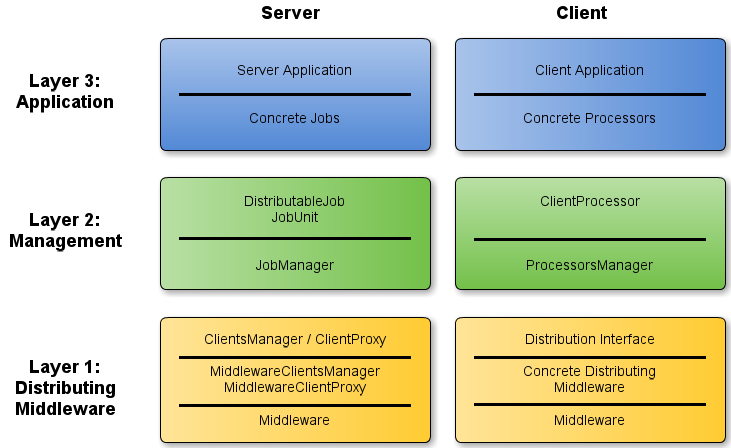
\includegraphics[scale=.4]{images/AbstractLayers-FuD.png}
	      \end{center}
	\end{frame}

	\begin{frame}\frametitle{Trabajos de FuD}
		\begin{block}{DistributableJob}
			Es un concepto de trabajo abstracto que encapsula cualquier tarea que será computada y puede ser subdividido en tareas más
			pequeñas llamadas \textbf{JobUnits}.
		\end{block}
		
		\pause
		\begin{block}{JobUnit}
			Representa una computación concreta y atómica que será llevada a cabo por alguno de los nodos de procesamiento. La tarea en 
			sí es representada por un mensaje el cual será pasado a un cliente de procesamiento quien se encargará de computarla.
		\end{block}
		
		\begin{center}
			%se pone asi para que \pause tenga efecto sobre la imagen
			\visible<2>{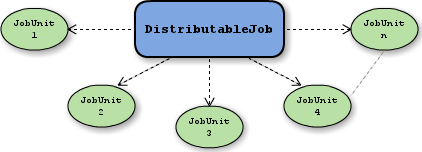
\includegraphics[scale=.4]{images/trabajos-fud.png}} 
		\end{center}
	\end{frame}
	
\end{subsection}

\begin{subsection}{Computación Voluntaria}

	\begin{frame}\frametitle{Computación Voluntaria}
		\begin{block}{Definición}
			La computación voluntaria es un tipo de computación distribuida donde personas (voluntarios) donan los recursos libres de 
			su ordenador a proyectos científicos mediante una conexión a internet.
		\end{block}
		
		\begin{center}
			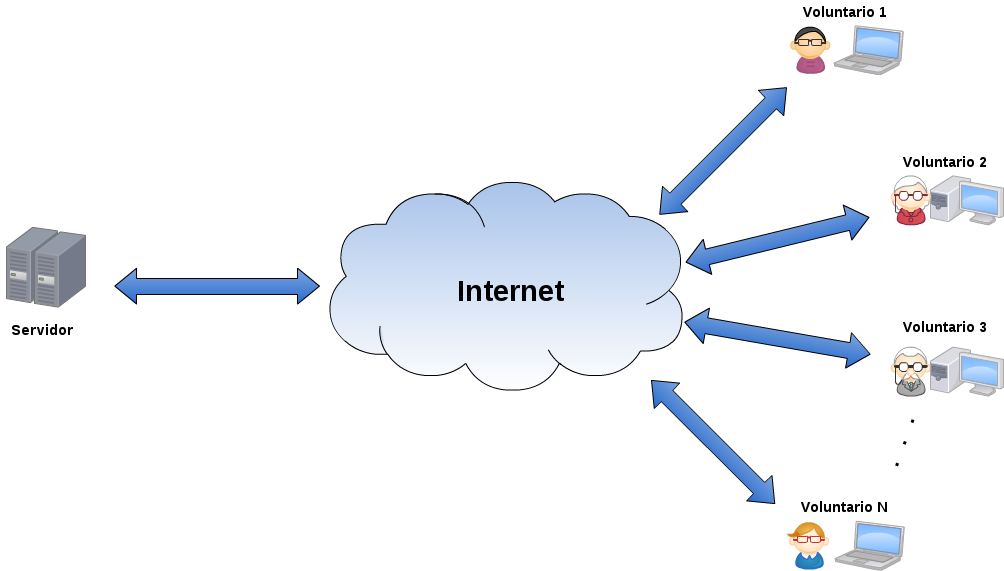
\includegraphics[scale=.22]{images/graf-comp-volunt.png}
		\end{center}
	\end{frame}

	\begin{frame}\frametitle{Computación Voluntaria}
		\textbf{Ventajas:\\[.5cm]}
		\begin{itemize}
			\addtolength{\itemsep}{3mm}
		    \item Los voluntarios pueden colaborar desde cualquier punto geográfico.
		    \item Hace posible la existencia de proyectos de investigación a bajos costos.
		    \item Los voluntarios no necesitan ser usuarios avanzados de computadoras.
		    \item Permite obtener y superar el poder de cálculo de una súper computadora.
		\end{itemize}
	\end{frame}

	\begin{frame}\frametitle{Computación Voluntaria}
		\textbf{Desventajas:\\[.5cm]}
		\begin{itemize}
		\addtolength{\itemsep}{3mm}
			\item Aumenta el consumo de energía de los ordenadores clientes debido a que éstos reducen su consumo en su tiempo libre.
			\item Para lograr un buen desempeño del proyecto es necesario apelar a medios de comunicación para reclutar voluntarios.
			\item Los voluntarios pueden confiar en los proyectos pero el proyecto no puede confiar en ellos.
		\end{itemize}
	\end{frame}
	
\end{subsection}

\begin{subsection}{BOINC}

	\begin{frame}\frametitle{Berkeley Open Infrastructure for Network Computing (BOINC)}
		\begin{block}{}
			\textbf{BOINC} es una plataforma de software de código abierto para computación voluntaria y computación grid, 
			cuyo principal propósito es hacer posible la investigación científica.
		\end{block}
		\pause
		\vspace{4mm}
		\textbf{Características}
		\begin{itemize}
			\item Los voluntarios pueden computar desde distintas plataformas.
			\item Los usuarios pueden participar en varios proyectos a la vez.
			\item Sólo se asignan tareas a voluntarios que cuenten con los recursos necesarios.
			\item Asignación de trabajos bajo demanda por parte de los clientes.
		\end{itemize}
	\end{frame}

	\begin{frame}\frametitle{Trabajos BOINC}
		Los trabajos de BOINC se encapsulan bajo dos conceptos importantes:
		\pause
		\vspace{4mm}
		\begin{block}{Workunit}
			Describe y representa la tarea a ser computada por un cliente del proyecto. Cada una está asociada a una aplicación en
			particular y puede tener uno o más archivos de entrada relacionados.
		\end{block}
		\pause
		\vspace{4mm}
		\begin{block}{Result}
			Es una instancia de una workunit que se desea resolver. Precisamente es este result el que será enviado a los clientes
			de BOINC para su procesamiento. Cada workunit debe tener asociado al menos un result.
		\end{block}
	\end{frame}

	\begin{frame}\frametitle{Proyecto BOINC}
		\begin{block}{}
			Un \textbf{proyecto BOINC} es el encargado de manegar todo el proceso de computación distribuida. Permite la 
			administración de cuentas de usuarios, de aplicaciones y define cómo van a ser distribuidos los trabajos.
		\end{block}
		\pause
		\vspace{2mm}
		\textbf{Componentes de un proyecto:}
		\begin{itemize}
			\item Una base de datos
			\item Un sitio web
			\item Un servidor conformado por:
			\begin{itemize}
				\item Generadores de trabajos \textit{(work generators)}
				\item Aplicaciones
				\item Utilidades \textit{(ej: start, stop, status, xadd, update\_version)}
				\item Demonios \textit{(ej: validator, assimilator, file\_deleter, db\_purge)}
			\end{itemize}
			\item Un archivo de configuración 
		\end{itemize}
		\vspace{2mm}
		\begin{block}{}
			Todo proyecto se identifica por la URL de su sitio web.
		\end{block}	
	\end{frame}
	
	\begin{frame}\frametitle{Proyectos conocidos}
		\begin{itemize}
		\addtolength{\itemsep}{2mm}
			\item Seti@home\\ (\url{http://setiathome.ssl.berkeley.edu/})
			\item Climate Prediction\\ (\url{http://climateprediction.net/})
			\item LHC@Home\\ (\url{http://lhcathomeclassic.cern.ch/sixtrack/})
			\item Einstein@Home\\ (\url{http://einstein.phys.uwm.edu/})			
		\end{itemize}
		\vspace{6mm}
		Lista completa de proyectos BOINC:\\
		\url{http://boinc.berkeley.edu/wiki/Project_list/}
	\end{frame}
	

	\begin{frame}\frametitle{Cliente BOINC y BOINC Manager}
		\begin{block}{Cliente BOINC \texttt{(core client)}}
			Es la aplicación cliente de BOINC que corre como demonio en las computadoras de los participantes.
		\end{block}	
		\pause
		\textbf{Sus principales funciones son:}
		\begin{itemize}
			\item Mantener una conexión directa con el servidor del proyecto para recibir trabajos y enviar resultados.
			\item Descargar la aplicación necesaria para la computación de cada trabajo.
			\item Realizar la computación de cada tarea.
			\item Administrar la distribución de los recursos locales entre los proyectos adheridos.
		\end{itemize}
		\pause
		\vspace{2mm}
		\begin{block}{BOINC Manager}
			Es una aplicación que ofrece una simple interfaz gráfica mediante la cuál los voluntarios pueden controlar el 
			\textbf{cliente BOINC}.
		\end{block}	
	\end{frame}

	\begin{frame}\frametitle{Componentes de BOINC}
		\begin{center}
			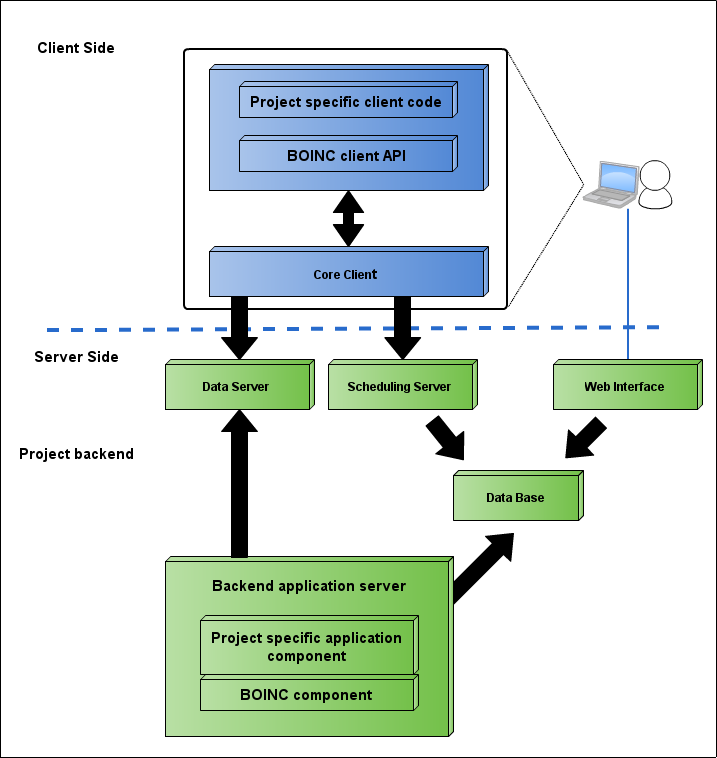
\includegraphics[scale=0.25]{images/componentes-boinc.png}
		\end{center}
	\end{frame}

	\begin{frame}\frametitle{Interacción entre servidor y cliente BOINC}
		\begin{center}
			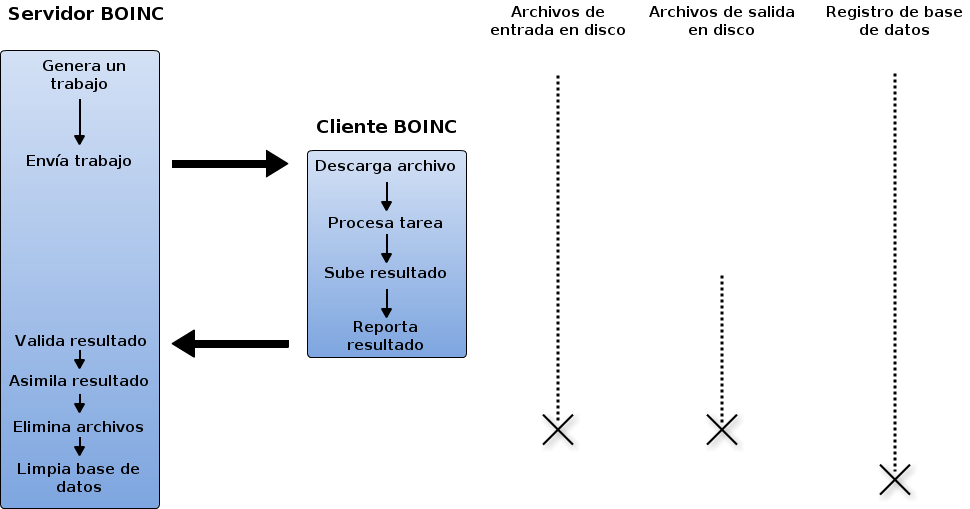
\includegraphics[scale=0.32]{images/Client-Server-Interact.png}
		\end{center}
	\end{frame}
	
\end{subsection}

		\chapter{Marco teórico}
\label{chapter:marco:teorico}


\section{Programación paralela}

La programación paralela es una técnica de programación basada en la ejecución simultánea de instrucciones tanto en un mismo ordenador con varios procesadores o bien en un clúster conformado por varios ordenadores haciendo uso de la computación distribuida.
Los sistemas multiprocesadores consiguen un aumento del rendimiento si se utilizan estas técnicas. En los sistemas monoprocesador el beneficio en rendimiento no es tan evidente debido a que la CPU es compartida por múltiples procesos en el tiempo.
\newline El mayor problema de la computación paralela radica en la complejidad de la comunicación y sincronización de las tareas involucradas en la computación, ya sea mediante secciones críticas, semáforos o paso de mensajes que permitan garantizar la exclusión mutua en las zonas del código en las que sea necesario.
\newline El paradigma de diseño y programación difiere mucho del utilizado para diseñar y programar aplicaciones secuenciales. Aquí, una buena estrategia de división del problema puede determinar la eficiencia de un algoritmo paralelo.

\subsection{Computación paralela}

Se denomina computación paralela al procesamiento simultáneo de datos. Ésto se logra dividiendo el problema original en partes más pequeñas de manera tal que cada elemento de procesamiento pueda ejecutar una parte del algoritmo al mismo tiempo que los demás. \newline La idea principal de la computación paralela es poder ejecutar más instrucciones en menos tiempo, por más que las instrucciones sigan tardando lo mismo.
Los elementos de procesamiento pueden ser diversos e incluir recursos tales como un único ordenador con muchos procesadores, varios ordenadores en red, hardware especializado o una combinación de los anteriores.
Resumiendo, el objetivo primordial de la computación paralela es aumentar la velocidad computacional y reducir los tiempos en la resolución de problemas.

\textbf{\newline \large Tipos de paralelismo}

\textbf{\newline Paralelismo a nivel de bit:} se basa en el incremento del tamaño de la palabra\footnote{una palabra es una cadena finita de bits que son manejados como un conjunto por el procesador. El tamaño o longitud de una palabra hace referencia al número de bits contenidos en ella.} del procesador. 
 Incrementando el tamaño de la palabra se reduce el número de instrucciones que el procesador debe ejecutar al efectuar operaciones con variables cuyos tamaños son mayores a la longitud de su palabra. Por ejemplo, en el caso en que un procesador de 32 bits deba efectuar una suma de dos variables enteras de 64 bits, primero debe sumar los 32 bits más bajos de cada entero y luego sumar los 32 bits restantes, efectuando de esta manera un total de dos instrucciones para para resolver una única operación. En cambio, 
 si el procesador fuera de 64 bits esta operación se ejecutaría con una simple instrucción.

\textbf{\newline Paralelismo a nivel de instrucción:} es una técnica que busca combinar las instrucciones de bajo nivel ejecutadas por el procesador con el fin de encontrar el mejor orden de ejecución que permita correr instrucciones de manera simultánea sin afectar el resultado final. La idea principal de utilizar esta técnica es poder aumentar la velocidad de ejecución y aprovechar al máximo la capacidad del hardware.
 
\textbf{\newline Paralelismo a nivel de datos:} consiste en subdividir los datos de entrada de un programa y ejecutar en diferentes procesos la misma secuencia de operaciones sobre cada subconjunto obtenido en la división. Es decir, cada procesador ejecuta la misma tarea sobre diferentes conjuntos de datos. Aquí, los datos se distribuyen y las tareas se replican.

\textbf{\newline Paralelismo a nivel de tareas:} es un tipo de paralelización que se centra en la distribución de tareas a través de diferentes nodos de procesamiento. Lo que pretende este tipo de paralelismo es realizar una división del conjunto de tareas en subconjuntos más pequeños para que sean
 ejecutadas por los distintos nodos disponibles en la computación.
 A esta técnica también se la conoce como ``paralelismo funcional''.

\textbf{\newline \large Características principales}

\begin{itemize}
 \item Se utilizan múltiples núcleos de procesamiento para la ejecución de las tareas.
 \item Los problemas son divididos en partes más pequeñas o subproblemas de tal manera para que puedan ser resueltos en paralelo.
 \item Los subproblemas obtenidos de la división son ejecutados simultáneamente en núcleos diferentes.\\
\end{itemize}


\textbf{\newline \large Tipos de sistemas paralelos más conocidos} \vspace{5 mm} \\
Las computadoras paralelas pueden ser diferenciadas según el nivel en que su hardware soporta paralelismo. Existe una gran variedad de arquitecturas que permiten la ejecución simultánea de múltiples instrucciones:

\textbf{\newline Computación multi-núcleo:} está dada por un procesador conformado por múltiples núcleos de procesamiento en un mismo chip. Un procesador multi-núcleo puede ejecutar múltiples instrucciones por ciclo desde múltiples flujos de instrucciones.

\textbf{\newline Multi-procesamiento simétrico:} es un sistema informático con múltiples procesadores idénticos que comparten la memoria y se conectan mediante un bus.

\textbf{\newline Computación distribuida:} se utilizan varios ordenadores interconectados a quienes se les envían diferentes tareas para su computación. Cada ordenador ejecuta localmente ese trabajo y al finalizar lo reporta al ordenador central logrando de esta manera una ejecución paralela y distribuida de tareas. En la siguiente sección se darán más detalles al respecto.

\subsection{Taxonomía de Flynn}

La taxonomía de Flynn es una clasificación de arquitecturas de computadoras propuesta por Michael J. Flynn en 1966.\\
Las cuatro clasificaciones definidas por Flynn se basan en el número de instrucciones concurrentes y en los flujos de datos disponibles en la arquitectura.\\
\texttt{Flynn} creó cuatro clasificaciones distintas considerando si los programas y computadoras operaban sobre una o múltiples instrucciones y si esas instrucciones utilizan un solo conjunto o múltiples conjuntos de datos.\\

\textbf{\newline \large La Clasificación}

\textbf{\newline (SISD) Una instrucción, un dato:} del inglés ``Single Instruction Single Data'', es la computación secuencial que no explota el uso de paralelismo en las instrucciones ni tampoco en el flujo de datos. Un ejemplo de esta clasificación son las máquinas monoprocesador.\\

\textbf{\\Gráficamente:}
\begin{figure}[H]
\begin{center}
  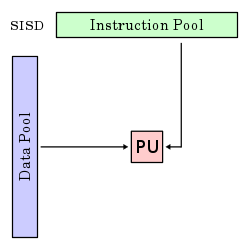
\includegraphics[scale=0.7]{images/SISD.png}
\caption{SISD}
\label{fig:SISD}
\end{center}
\end{figure} 

\textbf{\newline (SIMD) Una instrucción, múltiples datos:} del inglés ``Single Instruction Multiple Data'', es una arquitectura de computadora que explota múltiples flujos de datos en un único flujo de instrucciones para realizar operaciones las cuales pueden ser paralelizadas de manera natural. Por ejemplo: un GPU o un procesador vectorial el cual es capaz de ejecutar operaciones matemáticas sobre múltiples datos de forma simultánea.\\
\newpage

\textbf{\\Gráficamente: }

\begin{figure}[H]
\begin{center}
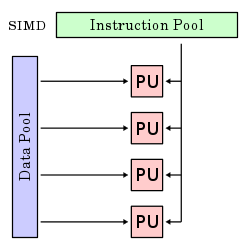
\includegraphics[scale=0.7]{images/SIMD.png}
\caption{SIMD}
\label{fig:SIMD}
\end{center}
\end{figure} 

\textbf{\newline (MISD) Múltiples instrucciones, un dato:} del inglés ``Multiple Instruction Single Data'', es una arquitectura que se utiliza cuando múltiples flujos de \linebreak instrucciones operan sobre un único flujo de datos. Esta arquitectura es poco común debido a que la efectividad de los múltiples flujos de instrucciones suele precisar de múltiples flujos de datos. Sistemas heterogéneos que operan sobre el mismo conjunto de datos y deben coincidir en resultados se suele utilizar en situaciones de paralelismo redundante, como por ejemplo en computadoras de control de navegación aérea, donde se necesitan varios sistemas de respaldo en caso de que uno falle.\\
\newpage 
\textbf{\\Gráficamente:}
\begin{figure}[H]
\begin{center}
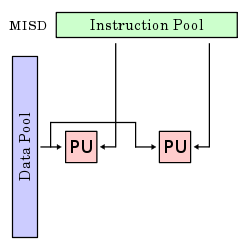
\includegraphics[scale=0.7]{images/MISD.png}
\caption{MISD}
\label{fig:MISD}
\end{center}
\end{figure} 

\textbf{\newline (MIMD) Múltiples instrucciones, múltiples datos:} del inglés ``Multiple Instruction Multiple Data'', esta arquitectura está conformada por múltiples procesadores autónomos que ejecutan simultáneamente diferentes instrucciones sobre conjuntos de datos diferentes. Los sistemas distribuidos por lo general son reconocidos en esta clasificación, ya sea explotando el uso de un único espacio compartido de memoria o bien uno distribuido.\\
\textbf{\\Gráficamente:}
\begin{figure}[H]
\begin{center}
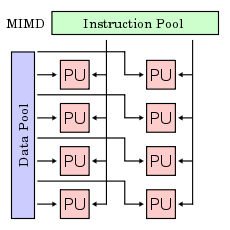
\includegraphics[scale=0.7]{images/MIMD.png}
\caption{MIMD}
\label{fig:MIMD}
\end{center}
\end{figure} 

El framework FuD presentado en la sección \ref{seccion:fud} tiene la capacidad de correr en máquinas con un diseño \textbf{MIMD}, con computadoras heterogéneas.


\subsection{Resolución de problemas paralelos}

El desarrollo de algoritmos paralelos aparece cuando tenemos un problema que requiere una gran capacidad de cómputo, ya sea por una gran cantidad de datos de entrada o por una gran complejidad en sus operaciones. El primer paso para el diseño de un algoritmo paralelo consiste en descomponer el problema principal en problemas más pequeños o subproblemas para que luego sean asignados a cada procesador y puedan ser ejecutados de manera independiente y simultánea.\\
No siempre es una buena decisión partir de un algoritmo secuencial intentando ``paralelizar'' la aplicación, sino que en ocasiones es necesario diseñar un nuevo algoritmo que seguramente será muy diferente al secuencial.

\textbf{\newline \large Descomposiciones más conocidas}

\textbf{\newline Descomposición de dominio o paralelismo de datos}: consiste en descomponer los datos de entrada de un programa 
paralelo en porciones más pequeñas e indivisibles de tal manera que posean aproximadamente el mismo tamaño. Cada una de estas porciones son asignadas a un procesador para su posterior ejecución. Se puede relacionar al paralelismo de datos con el modelo \textbf{SIMD} ya que permite mantener un único flujo de instrucciones.

\textbf{\newline Descomposición funcional}: se basa en la división del programa principal en subtareas más pequeñas donde cada una de éstas son asignadas y ejecutadas de manera independiente por cada procesador. En muchos casos, el número de subtareas obtenidas puede ser mayor a la cantidad de procesadores con los que se cuenta. \\
Este tipo de descomposición se implementa siguiendo un paradigma maestro-esclavo donde existe un proceso maestro que se encarga de enviar subtareas a los procesos
 esclavos. Cuando uno de estos últimos termina su computación, los resultados se envían al proceso maestro el cual nuevamente le asigna una nueva subtarea a procesar.
 Se prosigue de esta manera hasta agotar las subtareas pendientes.

\subsection{Modelos de programación paralela}

Los modelos de programación no están totalmente ligados a las arquitecturas paralelas pero sí estrechamente relacionados. Podríamos decir que cada arquitectura de computación paralela justifica esta relación haciendo uso de dichos modelos. Es por eso que un determinado modelos puede ser más eficiente que otro cuando se aplica sobre determinadas arquitecturas paralelas.\\
Existen básicamente dos modelos de comunicación de las plataformas paralelas \cite{gramagrubta}:

\textbf{\newline Espacios de direcciones compartidas \textit{(Shared Address Space)}}: se ve a los programas como una colección de procesos que pueden acceder a variables locales y globales almacenadas en un espacio de memoria compartido entre las diversas unidades de procesamiento. Cada proceso accede a dicha memoria a través de lecturas asincrónicas.\\
Este modelo es apropiado para el desarrollo de aplicaciones sobre arquitecturas de memoria compartida, aunque también puede ser utilizado para el desarrollo de aplicaciones sobre arquitecturas distribuidas, simulando un espacio de memoria compartido.

\textbf{\newline Paso de mensajes \textit{(Message Passing)}}: es una técnica empleada para aportar sincronización entre procesos y permitir la exclusión mutua de manera similar a como se hace con los semáforos, monitores, etc. Su principal característica es que no precisa de memoria compartida, por lo que es muy importante en la programación de sistemas distribuidos. Los elementos principales que intervienen en el paso de mensajes son: el proceso que envía, el que recibe y el mensaje.

\subsection{Equilibrio de carga}

Un aspecto fundamental que hay que tener en cuenta a la hora de desarrollar un programa paralelo es el \texttt{equilibrio de carga}.

Ésta es una metodología para distribuir equitativamente los trabajos a través de múltiples computadoras, clústers, procesos, redes de trabajos, discos, o todo aquello que conforme el sistema paralelo utilizado, de tal manera que se pueda asegurar el uso y la óptima distribución de los recursos para poder maximizar la salida, minimizar el tiempo de respuesta y evitar la sobrecarga en ciertos procesos cuando los demás se encuentren ociosos.

El equilibrio de carga se utiliza comúnmente para realizar comunicaciones internas en clústers o para implementar algoritmos de planificación en sistemas operativos.

\subsection{Etapas de diseño}

Las etapas de diseño de aplicaciones paralelas podrían resumirse entonces como sigue:
\begin{itemize}
 \item Identificar el trabajo que puede realizarse en paralelo.
 \item Diseñar la división y unificación del trabajo y datos entre procesos involucrados.
 \item Determinar el acceso a los datos, sincronizaciones y dependencias entre tareas.
 \item Asignar recursos de cómputo a los procesos que se ejecutarán en paralelo.
\end{itemize}


\section{Programación distribuida}

Un sistema distribuido se define como una colección de ordenadores autónomos conectados por una red y controlados por el software distribuido adecuado para que el sistema sea visto por los usuarios como una única entidad capaz de proporcionar facilidades de computación. El desarrollo de los sistemas distribuidos vino de la mano de las redes locales de alta velocidad
 a principios de \textit{1970}. Actualmente, la disponibilidad de computadoras personales de altas prestaciones, estaciones de trabajo y ordenadores servidores ha resultado en un mayor desplazamiento
 hacia los sistemas distribuidos respecto de los ordenadores centralizados multiusuario. Esta tendencia se ha acelerado por el desarrollo de software para sistemas distribuidos diseñado
 para soportar el desarrollo de aplicaciones distribuidas para permitir a los ordenadores coordinar sus actividades y compartir los recursos del sistema, hardware, software y datos.
Los sistemas distribuidos se implementan para hacer uso de diversas plataformas de hardware, desde unas pocas estaciones de trabajo conectadas por una red de área local, hasta Internet,
 que comunica a millones de ordenadores donde sus aplicaciones varían desde la provisión de capacidad de cómputo a grupos de usuarios, hasta sistemas bancarios, comunicaciones multimedia y
 abarcan prácticamente todas las aplicaciones comerciales y técnicas actuales. 

La programación distribuida es un tipo de programación paralela. Los programas paralelos pueden correr localmente y de manera coordinada, o bien estar separados en diferentes unidades de cómputo.
 Generalmente, en este último caso, los ordenadores suelen ser muy diferentes entre sí por lo que desarrollar este tipo de aplicaciones resulta en un mayor esfuerzo debido a nuevos factores que se
 deben tener en cuenta para mantener la calidad del software, como son la seguridad, extensibilidad, escalabilidad, tratamiento de fallos, concurrencia, transparencia del usuario frente a los componentes
 del sistema y heterogeneidad de los componentes  entre otros. Cuando se pretende resolver un problema de manera distribuida, el programa necesita ser dividido y cada parte resultante debe poder correr
 en diferentes ordenadores. Estos sub-programas corren simultáneamente y necesitan mantener una cierta comunicación entre sí que les permita avanzar con su respectiva tarea. 
Otro punto a tener en cuenta a la hora de desarrollar una aplicación distribuida es que si las aplicaciones van a correr en arquitecturas de hardware diferentes, 
estos programas tienen que ser compilados y optimizados específicamente para cada una.

\begin{center}
\begin{itshape}
 \textit{Programar un sistema distribuido significa escribir un programa para cada proceso tal que todos los programas en conjunto implementan la aplicación deseada \cite{VanRoyHaridi} }
\end{itshape}
\end{center}

La coordinación de estos procesos distribuidos puede ser una tarea complicada debido a que algunas unidades de trabajo pueden fallar o ser interrumpidas, o bien, los mensajes que contienen
 datos de entrada y/o resultados de la computación, podrían también no llegar a destino. Por consiguiente, si los programas se escriben sin contemplar estos casos, es probable que ante alguna
 situación de éstas, todas las computadoras involucradas en la resolución del problema terminen fracasando. En la programación distribuida, un proceso podría ser el proceso de control encargado 
de recibir y administrar los trabajos hechos por otros procesos, como es el caso de una arquitectura cliente-servidor donde el servidor debe manejar los requisitos de los clientes, o bien,
 todos los procesos podrían trabajar de manera peer-to-peer sin que exista un proceso maestro de control. Algunos ejemplos de problemas en donde se utiliza la programación distribuida para
 su resolución son, el análisis de datos geológicos sobre recursos como el petróleo, el modelado de proteínas y moléculas biológicas, la decodificación de mensajes, y simulaciones militares, entre otros.
 El proyecto \textsc{SETI} \footnote{\url{http://www.seti.org/}} encargado de buscar inteligencia extraterrestre utilizando ondas de radiofrecuencia capturadas desde la tierra quizás es uno de los mejores ejemplos.

Los sistemas distribuidos abarcan una cantidad de aspectos considerables, por lo cual su desarrollo implica mucha complejidad. En este modelo es muy importante que en las etapas de diseño y
 desarrollo se consideren dónde va a correr el sistema y cómo va a ser utilizado. Para ello, es necesario identificar ciertos puntos que son claves a la hora de diseñar y desarrollar una aplicación distribuida.
 Se debe identificar:

\begin{itemize}

 \item el tipo de Sistema Operativo sobre el cual correrá cada proceso,
 \item la red de comunicación que será utilizada,
 \item el lenguaje de programación que mejor se adapte a la solución del problema,
 \item qué debe hacer el servidor y qué debe hacer cada cliente,
 \item cómo actuar frente a pérdidas de mensajes, saturación en el tráfico, mensajes repetidos, 
 \item cómo mantener segura las conexiones,
 \item qué cantidad de clientes podrá manipular cada servidor,
 \item cómo descomponer el problema y cómo distribuir el trabajo de manera eficiente.

\end{itemize}
Estos puntos varían con cada problema sobre todo considerando los diferentes criterios e interpretaciones con los cuales puedan ser abordados.

Es importante que todas las aplicaciones incluyan un alto nivel de fiabilidad, seguridad contra interferencias externas y que proporcionen privacidad de toda la información que manejen.\\
 
\textbf{\newline Características de las aplicaciones distribuidas}\\
\\Concurrencia: los recursos disponibles en la red puedan ser utilizados simultáneamente por los usuarios y/o agentes que interactúan en la red. Por ejemplo el acceso simultáneo a la base de datos de un servidor.\\
\\Carencia de reloj global: las coordinaciones para la transferencia de mensajes entre los diferentes componentes para la realización de una tarea, no tienen una temporización general, está más bien distribuida a los componentes.\\
\\Fallos independientes de los componentes: cada componente del sistema puede fallar independientemente, con lo cual los demás pueden continuar ejecutando sus acciones.
 Esto permite el logro de las tareas con mayor efectividad, pues el sistema en su conjunto continúa trabajando.

\subsection{Topología de los sistemas distribuidos}

La topología de red se define como la cadena de comunicación usada por los nodos que conforman una red para comunicarse. 
En sistemas distribuidos, el término ``topología'' puede ser considerado y analizado en diversos contextos: físico, lógico o en términos de la comunicación, entre otros. Un caso particular es considerar la topología bajo el contexto del flujo de información. \\
Las topologías más comunes en este contexto son:

\begin{itemize}

 \item \textbf{Centralizada o Estrella}:

La topología estrella es uno de los tipos de topologías más utilizado donde generalmente las aplicaciones son vistas bajo una arquitectura cliente-servidor usado por servidores web, bases de datos y una amplia cantidad de sistemas distribuidos. Aquí, múltiples clientes se conectan a un único servidor quien es el encargado de centralizar y manejar toda la información disponible y de atender los requerimientos de los clientes. Por ejemplo, el proyecto \textsc{SETI@Home} es una arquitectura totalmente centralizada donde el servidor es el encargado de generar trabajos que luego serán computados por sus clientes. Entre sus ventajas se pueden mencionar: 

\begin{itemize}
\item si una PC se desconecta, o la conexión se pierde, solo queda fuera de la red esa PC,
\item resulta sencillo agregar y reconfigurar un nuevo ordenador,
\item es fácil prevenir daños o conflictos.
\end{itemize}

Una desventaja importante de esta topología es que si el nodo central falla, toda la red deja de transmitir.\\

\textbf{Gráficamente: }

\begin{figure}[H]
\begin{center}
  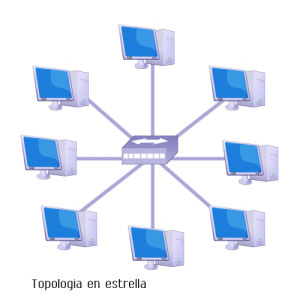
\includegraphics[height=2.5in,width=2.5in]{images/star.png}
\caption{Topología-estrella }
\label{fig:Estrella}
\end{center}
\end{figure} 

 \item \textbf{Anillo}:

En ocasiones, un único servidor centralizado no es capaz de manejar altas cargas de clientes, por lo que una solución común es utilizar un conjunto de ordenadores conectados en forma
 de anillo actuando como un único servidor distribuido. Aquí, cada estación está conectada a la siguiente y la última está conectada a la primera.
 Cada estación, además, tiene un receptor y un transmisor que hace la función de repetidor pasando la señal a la siguiente estación. En este tipo de red la comunicación
 se da por el paso de un token encargado de distribuir paquetes de información evitando de esta manera eventuales pérdidas de información debidas a colisiones.\\

\textbf{Gráficamente: }

\begin{figure}[H]
\begin{center}
  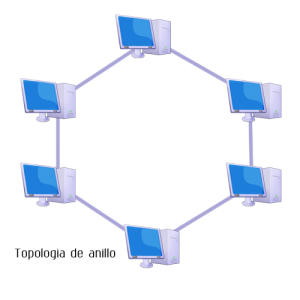
\includegraphics[height=2.5in,width=2.5in]{images/ring.png}
\caption{Topología-anillo }
\label{fig:Anillo}
\end{center}
\end{figure} 

 \item \textbf{Jerárquica o Árbol}

La topología jerárquica, también conocida como topología de árbol, tiene una larga historia en internet. Aquí  se cuenta con nodos periféricos individuales, por ejemplo hojas, que requieren transmitir  y recibir  únicamente de otros nodos sin la necesidad de actuar como repetidores o regeneradores. Al contrario de las redes centralizadas, la función del nodo central se puede distribuir. Como en las redes centralizadas convencionales, los nodos individuales pueden quedar aislados de la red por un fallo puntual en la ruta de conexión del nodo.
En estos casos, si falla un enlace que conecta con un nodo hoja, ese nodo hoja queda aislado; si falla un enlace con un nodo que no sea hoja, la sección entera queda aislada del resto.

Un ejemplo de este tipo de topología es la inserción del servicio de internet desde el proveedor, pasando por el router, luego por un switch que puede derivar a otro switch u otro router o sencillamente a los hosts. El resultado final, es una red con apariencia de árbol porque desde el primer router se comienza a ramificar la distribución de internet dando lugar a la creación de nuevas redes o subredes tanto internas como externas.

El sistema jerárquico más conocido en internet es el Servicio de Nombres de Dominio, \texttt{DNS}.\\
\newpage

\textbf{Gráficamente: }

\begin{figure}[H]
\begin{center}
  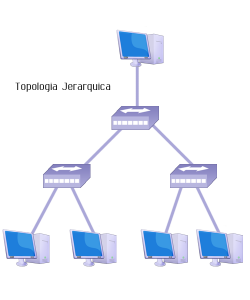
\includegraphics[height=2.5in,width=2.5in]{images/arbol.png}
\caption{Topología-arbol }
\label{fig:Arbol}
\end{center}
\end{figure} 

\item \textbf{Descentralizada}

Aquí, todos los nodos se comunican de manera simétrica y todos tienen las mismas funciones. Un ejemplo de este tipo de topología son las redes P2P, de las cuales Gnutella probablemente es el sistema puro descentralizado más conocido utilizado hoy en día. En las redes de este tipo, los nodos actúan como cliente y como servidor sin la necesidad de un servidor central que maneje las conexiones de red ni de un enrutador central que sirva como nodo y que administre direcciones. A esta topología también suele llamársela ``topología en malla''.
\newpage
\textbf{Gráficamente: }

\begin{figure}[H]
\begin{center}
  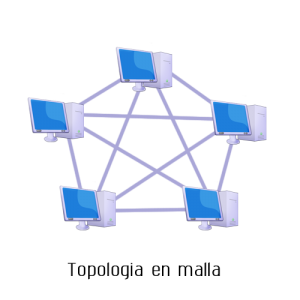
\includegraphics[height=2.5in,width=2.5in]{images/mesh.png}
\caption{Topología-decentralizada}
\label{fig:Decentralizado}
\end{center}
\end{figure} 

\item \textbf{Topologías Híbridas}

Las redes híbridas usan una combinación de dos o más topologías distintas de manera tal que la red resultante no tiene forma estándar. 
Por ejemplo, una red en árbol conectada a una red en árbol sigue siendo una red en árbol, pero dos redes en estrella conectadas entre sí  
muestran una topología de red híbrida. Estos tipos de redes se generan cuando se conectan dos topologías de red básicas. 

\textbf{Gráficamente: }

\begin{figure}[H]
\begin{center}
  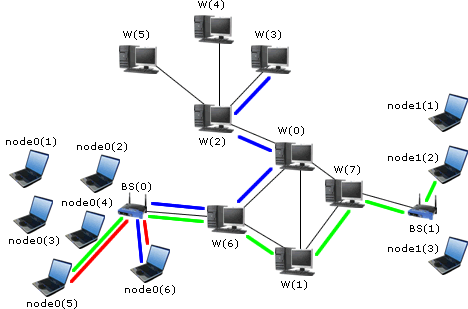
\includegraphics[height=2.5in,width=4.0in]{images/hibrida.png}
\caption{Topología híbrida}
\label{fig:Hibrida}
\end{center}
\end{figure} 

\end{itemize}

\subsection{Arquitectura cliente-servidor}

La arquitectura cliente-servidor de un sistema distribuido es el modelo más conocido y ampliamente adoptado en la actualidad. Consiste de una o varias aplicaciones servidoras,
 cada una actuando como un gestor de recursos y de una colección de aplicaciones clientes las cuales llevan a cabo tareas que requieren acceso a los recursos de hardware y/o software compartidos.
Los gestores de recursos a su vez podrían necesitar acceder a recursos compartidos manejados por otros procesos, es por eso que algunos procesos tienen ambos roles: son clientes y servidores a la vez. 

En este modelo, todos los recursos compartidos son mantenidos y manejados por los procesos servidores. Los procesos clientes realizan peticiones a los servidores cuando necesitan acceder a algún recurso.
Si la petición es válida, entonces el servidor lleva a cabo la acción requerida y envía una respuesta al proceso cliente.\\

Los servicios brindados varían de un sistema a otro, entre ellos se encuentran los siguientes:

\begin{itemize}
 \item  Ejecución de un determinado programa.
 \item  Acceso a un determinado banco de información.
 \item  Acceso a un dispositivo de hardware.
\end{itemize}

Esta arquitectura permite descentralizar el procesamiento y los recursos haciendo que ciertos servidores estén dedicados solo a una aplicación determinada y por lo tanto ejecutarla de manera eficiente.
Existen diversos tipos de servidores, entre los más comunes se encuentran los servidores de archivos, servidores de bases de datos, servidores web, servidores de correo, servidores de objetos, servidores de impresión, etc.


\section{Computación grid}

La computación Grid no es una nueva tecnología pero sí innovadora ya que representa una forma diferente de computación distribuida. Fue propuesta por Lan Foster y Carl Kesselman a mediados de los '90 como una revolucionaria técnica para resolver problemas complejos entre diversas organizaciones optimizando costos y tiempos. A partir del año 2000 se han hecho grandes progresos sobre dicha infraestructura y actualmente es cada vez más utilizada por organizaciones de todo el mundo.

Computación Grid puede tener varios significados para diferentes personas. La visión más general es presentada como una analogía a las redes de energía donde los usuarios tienen acceso a la electricidad a través de los enchufes de la pared sin importar ni considerar cómo y dónde se genera dicha energía. Esta visión presenta una idea donde la computación Grid se vuelve penetrante y los usuarios ganan acceso a recursos como les sea necesario sin tener conocimiento alguno sobre dónde se ubican dichos recursos o qué tipo de hardware y/o software poseen.

El término “Computación Grid” o simplemente “Grid” se enmarca dentro de la tecnología que permite agrupar un conjunto de recursos computacionales para resolver problemas de gran escala mediante el uso colectivo de ordenadores de escritorio, PDA, portátiles, móviles, redes, software, bases de datos, o instrumentos especiales como radios y telescopios. Es por ello que el propósito del grid es facilitar la correcta integración de todos estos recursos como un todo.
El control y mantenimiento central del Grid es llevado a cabo por un servidor que, generalmente, se encuentra replicado. Él es quien se ocupa de manejar y monitorizar el tráfico del sistema Grid encargándose de la entrega de los trabajos listos para procesar, de la recepción de resultados parciales y de la combinación de todos los resultados parciales para obtener el resultado final.

Puesto que los recursos que son compartidos pertenecen a diferentes usuarios, la seguridad pasa a ser un factor esencial en esta arquitectura centrándose en los siguientes aspectos:

\begin{itemize}
 \item \textbf{política de accesos:} define qué es lo que se va a compartir, a quién se le permite el acceso y bajo qué condiciones.
 \item \textbf{autenticación:} mecanismos para garantizar la identidad de un usuario o de un recurso concreto.
 \item \textbf{autorización:} procedimiento para averiguar si una determinada operación es consistente en base a las relaciones que se han definido previamente de cara a compartir recursos.
\end{itemize}

\textbf{Existen tres conceptos importantes que describen un Grid:}

\begin{itemize}
\item \textbf{visualización:} se refiere a la integración uniforme de sistemas heterogéneos geográficamente distribuidos que permiten a los usuarios hacer uso del Grid de manera transparente. Los nodos que conforman el Grid no están centrados geográficamente en un punto 	particular sino que están distribuidos en múltiples dominios y pueden ser accedidos a través de redes de área extensa, como por ejemplo Internet. Esta distribución implica que un usuario del Grid puede tener acceso directo a dichos nodos sin importar su ubicación pudiendo de esta manera extraer los recursos que requiera para el cómputo. Por ello, desde la perspectiva del usuario, hay un solo punto de entrada al sistema Grid.
\item \textbf{heterogeneidad:} representa la heterogeneidad de los recursos que forman las organizaciones virtuales que conforman al Grid. Es decir, que dichas organizaciones están compuestas por nodos de procesamiento que poseen hardware, software y sistemas operativos diferentes.
\item \textbf{dinámico:} los recursos pueden unirse o abandonar una organización virtual según conveniencia.
\end{itemize}

La principal utilidad del Grid es proveer de manera eficiente altas prestaciones de procesamiento con el fin reducir los tiempos en la resolución de problemas que requieren una gran capacidad de cómputo.

\begin{center}
\textit{“Grid es un súper-ordenador virtual que permite ejecutar aplicaciones que no pueden ser soportadas eficientemente en un único ordenador”}
\end{center}

\textbf{Clasificación de la Computación Grid:}

Podemos encontrar diversos tipos de Computación Grid. Éstos se clasifican según los servicios y recursos que ofrecen a los usuarios:

\begin{itemize}

\item \textbf{Grid Computacionales:} permite el acceso a los llamados “súper-computadores” para realizar tareas que requieren tiempos de cálculos muy elevados.
  
\item \textbf{Grid específicos:} en esta clasificación se engloban los Grids utilizados para ciertas investigaciones sobre temas específicos. 
Algunos de los temas para los que se utilizan son farmacéutica, química, astrofísica, tratamiento y representación de videos, simulación del clima, geología, etc.

\item \textbf{Grid de datos:} orientado principalmente para un almacenamiento y replicado de datos desde sitios ubicados en distintos sectores geográficos. Su funcionalidad se centra en obtención, catalogación, replicación y la coordinación de grandes cantidades de datos.

\item \textbf{Grid de servicios:} su funcionalidad se centra en proporcionar a los clientes recursos y aplicaciones desde cualquier componente de 
la arquitectura Grid a través de alguna política de disponibilidad (autoría, reconocimiento, etc.).

\item \textbf{Grid de recursos:} a diferencia del anterior, su funcionalidad se centra en proveer a los usuarios el uso de recursos concretos tales como capacidad de cómputo, ciclos de CPU, etc. desde un sector o área específica de la arquitectura grid.

\end{itemize}

\vspace{0,5cm}

\textbf{Características de la computación Grid:}

\begin{itemize}
\item \textbf{capacidad de equilibrio de sistemas:} los usuarios no necesitan calcular la capacidad de cómputo de los ordenadores a la hora de la entrega de trabajos ya que si ese ordenador no posee los recursos suficientes para llevarlo a cabo, el middleware reasignará el trabajo a otro ordenador.
\item \textbf{bajo costo:} brinda el poder de un súper-computador a un bajo costo ya que se dispone de una ``Grilla'' de recursos. No es necesario disponer de grandes servidores sino que se hace uso de componentes de bajo costo como lo son las PC de escritorio, laptops, etc.
\item \textbf{alta disponibilidad:} Si uno de los servidores falla, se reasignarán sus servicios a los servidores restantes.
\item \textbf{tolerancia a fallos:} si uno de los nodos del Grid falla, el sistema lo reconoce y reasignará la tarea a otra máquina. 
\item es una estructura flexible a los cambios.
\item no necesita de nuevas estructuras o arquitecturas para que funcione.
\end{itemize}

\vspace{0,5cm}

\textbf{Proyectos más conocidos que hacen uso de la Computación Grid:}

\begin{itemize}
  
\item SETI@Home \url{http://setiathome.berkeley.edu/}
\item Folding@Home \url{http://folding.stanford.edu/Spanish/Main/}
\item EGEE \url{http://public.eu-egee.org/}
\item IrisGrid \url{http://www.irisgrid.es/}
\item EELA \url{ http://www.eu-eela.org/}
\item EUFORIA \url{http://www.euforia-project.eu/}

\end{itemize}

\vspace{0,5cm}

\textbf{ Herramientas para implementar proyectos Grid:}

\begin{itemize}
 \item  BOINC \url{http://boinc.berkeley.edu/}
 \item  Advance Resource Connector \url{http://www.nordugrid.org/middleware/}
 \item  Load Sharing Facility \url{http://www.platform.com/Products/platform-lsf-family/}
 \item  Parallel Virtual Machine \url{http://www.csm.ornl.gov/pvm/pvm_home.html}
 \item  Globus Toolkit \url{http://www.globus.org/}
\end{itemize}

\textbf{Características de los servicios ofrecidos por la infraestructura del grid:}

\begin{itemize}
\item Servicios seguros en cuanto a capacidad de cómputo, integridad de datos, acceso a recursos, etc.
\item Servicio consistente basado en estándares evitando la heterogeneidad en el acceso a datos y operaciones.
\item Servicio penetrante ya que desde cualquier ubicación se puede acceder a sus recursos y extraer la potencia que se requiera.
\item Servicio económico lo que permite que llegue a más organizaciones haciendo que esta tecnología se universalice.
\end{itemize}


\subsection{Arquitectura de un sistema Grid}

Para lograr conseguir una imagen comprensible y coherente de la arquitectura de un sistema Grid es necesario primeramente identificar aquellos 
servicios que son necesarios en todo sistema y que, precisamente, son los que brindan las propiedades y características más destacadas.  

\subsubsection{ Servicios requeridos }

Para hacer posible que la ejecución de un trabajo sea satisfactoria se requieren de unos servicios que provean la funcionalidad que este trabajo requiera: 

\begin{itemize}

\item Por ejemplo, un usuario debe poder identificarse. Con este servicio el usuario puede certificar que es realmente quien dice ser, y
 asimismo el recurso que se quiere utilizar deberá autenticarse para que el usuario tenga la seguridad de que se ejecuta donde quiere, por lo que hablamos de autenticación mutua.
\item Un servicio de autorización es necesario, también para permitirle a un usuario la ejecución de tareas sobre un recurso, autorizándose como un usuario local, 
con sus permisos y restricciones dependiendo del contexto, la hora de petición o ejecución, etcétera.
\item Un servicio de planificación o  scheduling de los recursos, para que la utilización de los mismos sea eficiente y haya un reparto equitativo.
\item Asimismo es necesario un servicio para  descubrir recursos, ya que en un entorno de estas características se pueden añadir y quitar los mismos por
 lo que su selección debe ser dinámica.
\item También es recomendable un servicio de reserva anticipada, para poder ejecutar en un grupo de recursos en los que normalmente no es posible hacerlo,
 y que debe compenetrarse con el servicio de planificación.
\item Un servicio de  acceso a datos remotos, necesario para obtener los datos requeridos por un programa en ejecución ya que éstos pueden ser muy numerosos.
 Puede ser necesario un servicio de  réplica  para hacer copias de datos que sean muy “caros” de  transportar y que pueda ser conveniente tener en una localización más cercana.
\item Además se debe contar con recursos para hacer transferencias rápidas de estos datos.
\item Los servicios de  monitorización  son necesarios para controlar la correcta ejecución de los distintos trabajos, así como para controlar si los diferentes 
servicios que hemos comentado se encuentran disponibles y corriendo correctamente para su utilización.

\end{itemize}

\subsubsection{Arquitectura global}

La arquitectura global del sistema puede dividirse en diferentes piezas, dependiendo de los diferentes niveles en los que actúe cada componente. Ésto nos dará un típico modelo de arquitectura en capas.

\begin{figure}[H]
\begin{center}
  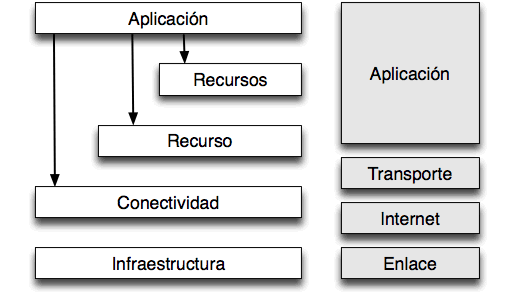
\includegraphics[height=3.0in,width=4.0in]{images/arquitectura-grid.png}
\caption{Arquitectura-Global}
\label{fig:Arquitectura}
\end{center}
\end{figure}

\begin{itemize}
 \item  En el nivel más bajo encontramos los servicios que son aplicables al control de los recursos locales, es lo que se denomina la capa \textbf{fábrica} o \textbf{infraestructura}.
 En esta capa se modelan los recursos accesibles, aquellos como:

      \begin{itemize}
      \item Recursos computacionales, como por ejemplo un clúster o un simple computador personal.
      \item Sensores, instrumentos de laboratorio.
      \item Sistemas de almacenamiento de datos.
      \item Sistemas de archivos distribuidos.
      \end{itemize}

      La funcionalidad básica que deben proveer, y de la que dependen capas superiores es la que nos da información sobre los recursos que está 
      modelando y de qué manera están disponibles para su utilización. Por ejemplo, para recursos computacionales debe:

      \begin{itemize}
      \item proveer información sobre el Hardware y el Software disponible, sobre el estado actual, carga, utilización, disponibilidad etcétera.
      \item monitorizar procesos que se estén ejecutando.
      \item un valor opcional podría ser la posibilidad de reservar el recurso.
      \item controlar recursos asociados a procesos.
      \item dar información sobre el estado de una posible cola de ejecución en la que residan los procesos.
      \end{itemize}

\item  En el siguiente nivel, nos encontramos con la capa de \textbf{Conectividad}, que tiene como función proveer los métodos y protocolos de comunicación entre los 
recursos modelados en la capa anterior. Aquí, los protocolos y la seguridad son muy importantes ya que es un requerimiento básico para el correcto funcionamiento del sistema. 
En esta capa se encuentran servicios que proveen los medios adecuados para hacer posible la comunicación a cualquier middleware o aplicación que se encuentre por encima de estos.

\item La siguiente capa es la denominada de \textbf{Recurso}, y es la encargada de compartir y gestionar los recursos individuales mediante la utilización de protocolos sobre la capa anterior de conectividad. En esta capa se definen los protocolos que permiten monitorizar, controlar y negociar operaciones que requieren un único recurso mediante los servicios subyacentes. 
Además, se llevarán a cabo la iniciación de las transacciones que sean necesarias para la realización del trabajo, tales como la comunicación 
del ejecutable en el recurso en el que se vaya a ejecutar, así también como la localización y recuperación de aquellos datos que sean necesarios para la ejecución.
También debe ser posible realizar en esta capa el control de los trabajos, proporcionando los métodos para reiniciar, relocalizar o cancelar un trabajo. 
Dentro de este control también podemos incluir en parte los servicios de Accounting, quienes permiten llevar un registro estadístico de las aplicaciones que 
se han corrido en un determinado recurso.

\item  La siguiente capa es la denominada capa de \textbf{Recursos}, y tiene como finalidad la coordinación de múltiples recursos accesibles por la capa anterior. En esta capa podemos encontrar, por ejemplo, aquellos servicios de información y directorio que nos dan una idea global del sistema y  mediante los cuales podemos localizar los recursos necesarios. La función principal aquí es la de utilizar los protocolos de comunicación de información de la capa anterior para proveer una vista global de los recursos. Aquí se sitúan servicios como los de \textit{scheduling}, \textit{co-allocation}, y \textit{brokering}. Estos servicios proveen los métodos para buscar aquellos recursos que se adaptan a las necesidades de nuestros trabajos, conociendo algunos datos sobre los mismos e intentando optimizar la asignación global mediante métodos de búsqueda o brokering. Con los servicios de \textit{co-allocation} podemos hacer reservas simultáneas de aquellos recursos que son necesarios para la consecución correcta del trabajo.

      \textbf{Existen tres tipos distintos de scheduler distribuido:}
      \begin{itemize}
      \item  Planificador de trabajos, encargado de maximizar los trabajos realizados por unidad de tiempo.
      \item  Planificador de recursos, encargado de llevar al máximo posible el uso de los recursos disponibles.
      \item  Planificador de la aplicación, encargado de dividir la aplicación en tareas, asignar los recursos necesarios para su ejecución y monitorizar el desarrollo de los mismos.
      \end{itemize}

      Los dos primeros intentan asegurar la eficiencia del grid, mientras que el tercero se enfoca exclusivamente en la efectividad de la aplicación.\\

      Esta capa también puede incluir servicios de replicación de datos, por ejemplo en caso de que estuvieran en una localización lejana.
      Las capas más altas como las aplicaciones o servicios más complejos del middleware deben utilizar los servicios que se provean en esta capa para la programación del grid. 

\item La siguiente y última capa es la denominada de \textbf{aplicación}, la cual se enfoca a la definición de protocolos que permitan a las aplicaciones acceder al grid a 
través de las distintas capas. Según el tipo de aplicación que sea, puede ser necesario conectarse a través de todas las capas o acceder directamente a alguna de ellas. 

\end{itemize}

\subsection{Scheduling y Scavenging}

El Grid es responsable de enviar trabajos a determinadas máquinas para que sean ejecutados. En el más sencillo de los casos,
 un usuario puede seleccionar la máquina adecuada para ejecutar el trabajo y luego, ejecutando un comando, envía el trabajo a dicho ordenador. 
En sistemas Grid más complejos se debe incluir un “job scheduler” o planificador de trabajos para que se encargue automáticamente de encontrar 
las máquinas adecuadas para ejecutar las tareas en espera.

En un sistema Grid “\textbf{scavenging}” cualquier máquina que esté ociosa reportará su estado al servidor quien le asignará un nuevo trabajo acorde a los requerimientos de dicha tarea.
Aquí, si la máquina ocupa sus recursos en algún proceso local, no perteneciente al Grid, el trabajo enviado generalmente es suspendido o 
bien retrasado provocando cierta incertidumbre en los plazos de tiempos que toma la resolución de cada trabajo en el Grid.

\subsection{El Resource-Broker}

El \textbf{Resource Broker} (\textbf{RB}) representa el núcleo del Grid y su tarea consiste en identificar y caracterizar dinámicamente los recursos disponibles más 
apropiados para luego asignarles los trabajos generados. El \textbf{RB} opera sin un control global y sus decisiones están basadas en la información ofrecida por cada recurso
 individual y en los servicios de información de recursos agregados. Además de la información sobre los recursos disponibles, cada máquina puede proveer información 
estática acerca del tipo de arquitectura, configuración de memoria, frecuencia de CPU, sistema operativo, etc. como así también información dinámica tales como la carga
 actual y el estado de la cola de lotes de trabajos.

\textbf{Cómo trabaja el Resource Broker:}

Para explicarlo, partamos de que un usuario tiene un problema donde las necesidades computacionales exceden sus recursos. 
Para solucionarlo implementa trabajos que se puedan ejecutar sobre un Grid. El usuario se conecta y se valida en el sistema Grid. 
Una vez que el usuario está conectado, se comunica con el \textbf{Resource Broker} el cual se encarga de enviar un requerimiento al servidor de información del Grid,
para obtener detalles acerca de los recursos de hardware y software que están disponible, y al “\textbf{Replica Catalog}” para conocer la ubicación de toda la información existente. 
Con todo lo obtenido, el Resource Broker elige el recurso más adecuado al cual le asignará los trabajos a ser ejecutados. 
Una vez finalizada la computación, es el mismo \textbf{Resource Broker} quien se encarga de enviar los resultados obtenidos nuevamente al usuario.\\

\textbf{Replica Catalog:} provee la ubicación en el sistema grid de las distintas réplicas de un grupo de datos determinado. 


\section{Computación voluntaria}

La computación voluntaria es un tipo de computación distribuida donde cada voluntario, mediante una conexión a Internet, dona los recursos libres de su ordenador a uno o varios proyectos científicos de investigación con el fin de incrementar su poder computacional.

Los orígenes de la computación voluntaria se remontan a Enero del 1996, cuando un grupo de investigadores alistó participantes al proyecto “Great Internet Mersenne Prime Search (GIMPS)” en su búsqueda de números primos cada vez mayores.
En 1999 se lanzaron los proyectos SETI@home un proyecto que busca indicios de vida extraterrestre y Folding@home un simulador de “plagamiento de proteínas”. Entre 1998 y 2002, se formaron varias compañías las cuales utilizaban computación voluntaria.  
En el 2002 el proyecto Berkeley Open Infrastructure for Network Computing (\textit{BOINC}) fue fundado y se convirtió en el software que más se ejecuta sobre la red pública. Hoy en día existen varios proyectos de computación voluntaria aplicados en distintas áreas tales como  Biología, estudio del Clima, análisis de epidemias, física entre otros.
 Todos ellos utilizan el middleware \textit{BOINC}.\\

La computación voluntaria generalmente se aplica en proyectos académicos o universitarios desarrollados principalmente para la investigación científica. 
Es muy importante para las organizaciones la difusión de sus proyectos, dar a conocer los trabajos que realizan y sus metas de tal manera que las personas se vean incentivadas a participar  como voluntarios y que los científicos puedan lograr un mayor poder computacional.\\

En la actualidad, la cantidad de proyectos de computación voluntaria crece rápidamente por lo que se requieren constantes mejoras en este paradigma.
Para lograr ésto e incrementar la productividad de la computación voluntaria se deben tener en cuenta dos puntos importantes:\\

\begin{enumerate}
 \item \textbf{Mejorar el uso de los ciclos de CPU donados por los voluntarios para que la computación sea más efectiva:}
  apunta a que las políticas para el manejo de tareas y resultados que son enviados a los clientes sean mucho más efectivas.
  Hasta el momento los proyectos utilizan una de las dos políticas existentes.
  La primera se conoce como Buffer None y propone que los clientes reciban de a una tarea a la vez y en el momento de enviar el resultado de la tarea recibir la siguiente tarea; 
  la segunda es conocida como Buffer N Days donde los clientes reciben y almacenan en un buffer a un conjunto de tareas para luego procesarlas. 
  Una vez que el buffer queda vacío se vuelve a requerir un nuevo conjunto de tareas.\\

  \item \textbf{Explorar diferentes caminos para incrementar la cantidad de recursos donados:} 
en este punto se pretende aumentar el número de recursos o ciclos de CPU que son donados a los proyectos. 
Para ello, generalmente, se opta por expandir los proyectos de tal manera que la aplicación cliente del proyecto pueda ejecutarse
 en otros recursos más allá de las computadoras personales, como por ejemplo consolas de videos juegos, redes de computadoras, súper-computadoras, etc.
 Tal es el caso de Folding@home, el cual puede tener colaboradores que participen desde las consolas de juegos Sony “PlayStation 3” la cual en su sistema 
trae una sección para instalar el cliente de dicho proyecto.\\

\end{enumerate}

\textbf{Algunos de los proyectos más conocidos que trabajan con computación voluntaria son:}\\

\begin{itemize}
 \item Distributed.net \url{http://distributed.net/}
 \item Seti@home \url{http://setiathome.ssl.berkeley.edu/}
 \item Folding@home \url{http://folding.stanford.edu/}
 \item The Great Internet Mersenne Prime Search (GIMPS) \url{http://www.mersenne.org/}
\end{itemize}

Los impulsores de la computación voluntaria sostienen que dado el enorme número de ordenadores personales que hay en el mundo, más de 1000 millones,
este nuevo modelo supone más capacidad de cálculo para la ciencia que cualquier otro tipo de computación y que el diferencial a favor de la computación
 voluntaria aumentará con el tiempo porque los consumidores de ordenadores personales y consolas crecerán más rápido que los de recursos más especializados. 
Es importante destacar que la computación voluntaria no pretende desplazar a otros paradigmas de computación como lo son los sistemas grid
o las infraestructuras de súper-computación pero sí consolidarse como un recurso más para el cálculo científico.\\

\textbf{Características de la computación voluntaria:}
\begin{itemize}
 \item permite a personas colaborar con la ciencia siendo ellas la principal fuente para la obtención de recursos de cálculo.
 \item hace posible la existencia de proyectos de investigación a bajo costo.
 \item permite obtener y superar el poder de cálculo de una súper-computadora.
 \item los voluntarios no necesitan ser usuarios avanzados de computadoras ya que el software necesario para contribuir es simple de instalar y evita configuraciones específicas de sistemas operativos.
 \item alienta el interés público en la ciencia.
 \item impulsa a los científicos publicar sus investigaciones en términos accesibles a fin de sumar voluntarios a sus proyectos.
 \item ayuda a contribuir al avance del conocimiento en cuestiones de interés personal.
\end{itemize}

\vspace{5mm}

\textbf{Costos y desventajas de la computación voluntaria:}

\begin{itemize}
 \item aumenta el consumo de energía de los ordenadores clientes debido a que éstos reducen el consumo en su tiempo libre.
 \item para lograr reclutar voluntarios y un buen desempeño del proyecto se necesita apelar a medios de difusión.
 \item los voluntarios pueden confiar en los proyectos pero el proyecto no puede confiar en ellos ya que éstos son anónimos.
 \item es una nueva tecnología que está en auge por lo que todavía no es muy conocida en el ámbito de la investigación en comparación con computación distribuida, clústers o Grid.
\end{itemize}

\subsection{Interacción cliente-Servidor}

Los proyectos de computación voluntaria son desarrollados utilizando un modelo arquitectural cliente-servidor donde utilizan uno o varios servidores.
En el contexto de la computación voluntaria, las tareas son un conjunto de datos llamados workunit.

\subsubsection{El servidor}

El servidor tiene varias responsabilidades en la participación del proyecto. 
En él reside el sitio web del proyecto mediante el cual brinda información al público en general y los voluntarios descargan
 la aplicación cliente necesaria para iniciar la colaboración. Además, en él se almacena la base de datos del proyecto con toda la información
 de los clientes como así también los trabajos enviados y resultados obtenidos. 
La principal funcionalidad del servidor es manejar los trabajos de la aplicación. Dicha tarea consiste en: a partir de un problema que requiere una gran capacidad de cómputo para resolverlo, se desarrolla una aplicación servidora encargada de dividir el problema en partes más pequeñas donde cada una de ellas se asocia con una tarea cuya ejecución devuelve la solución a ese subproblema. Para ello, cada tarea se distribuye sobre los voluntarios disponibles quienes mediante la aplicación cliente del proyecto ejecutan dichas tareas localmente para luego informar cada resultado obtenido. Una vez que el servidor cuenta con todos los resultados parciales, el mismo se encarga de validarlos y verificar que son resultados correctos para luego combinarlos y obtener así el resultados final.

\subsubsection{El cliente}

El cliente tiene como responsabilidad principal la ejecución de las tareas enviadas por el servidor. Cuando la computadora del voluntario entra en estado ocioso 
la aplicación cliente del proyecto le envía un requerimiento al servidor del proyecto solicitando trabajos.
 El servidor acepta ese requerimiento y le envía uno o varios trabajos a procesar dependiendo de la política adoptada por el proyecto. 
Una  vez finalizada la ejecución del  trabajo, el cliente le envía los resultados al servidor para luego requerir más trabajos.
Debemos destacar que las computadoras de los voluntarios siempre deben estar ociosas para que utilice su tiempo libre computando 
las workunit que el servidor le asignó; en el contexto de la computación voluntaria, una computadora se considera ociosa si se está ejecutando 
su protector de pantalla). Si el usuario comienza a utilizar la computadora mientras la aplicación cliente está procesando, 
ésta se suspende hasta que la computadora vuelva al estado ocioso.

Algunos proyectos de computación distribuida adoptan un modelo “push” donde el servidor inicia la comunicación con el cliente generando
 conexiones entrantes en contra-posición con el modelo “pull” donde es el cliente quien envía requerimientos entrantes al servidor.
Este último modelo es el adecuado y necesario en computación voluntaria ya que los clientes pueden estar detrás de firewalls y otros 
elementos de red que impidan una comunicación directa hacia el cliente provenientes desde el servidor.

\begin{figure}[H]
\begin{center}
  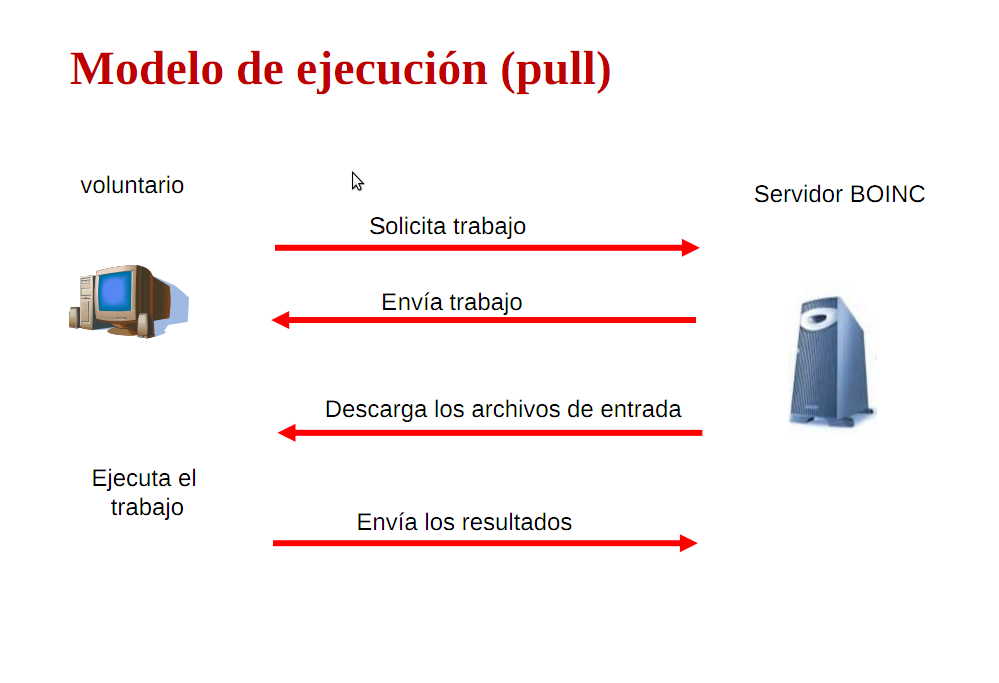
\includegraphics[height=3.5in,width=5.0in]{images/pull.png}
\caption{ Modelo de interacción cliente-servidor BOINC}
\label{fig:pull}
\end{center}
\end{figure} 

\subsection{Tolerancia a los hackers}

Los usuarios que colaboran con proyectos sobre computación voluntaria son anónimos por lo que sólo deben ingresan los datos típicos de una cuenta 
como alguna dirección de e-mail, país, etc. para poder participar. No hay control ni seguimiento de la forma en que el usuario colabora en el proyecto. 
Si entre ellos existen ciertos usuarios mal intencionados cuya meta es simplemente perjudicar el proyecto enviando resultados erróneo o pidiendo crédito 
por trabajos que no realizaron, éstos no pueden ser despedidos ni acusados. Es por eso que en los proyectos se deben tomar ciertos recaudos ante la 
posibilidad de tales malos comportamiento.  Uno de los métodos más utilizados es un sistema de firmas digitales, de tal manera que los hackers 
no pueden robar información. Un método para evitar resultados erróneos es enviar el mismo trabajo a dos máquinas diferentes y comparar resultados, 
de tal manera que estos y sus créditos sean aceptados si ambos se corresponden.

\subsection{Middleware para la computación voluntaria}

Las primeras aplicaciones para la computación voluntaria eran programas que combinaban una estructura para la computación científica y la computación
 distribuida con una arquitectura inflexible sobre la cual era muy complicado desarrollar nuevas aplicaciones o versiones.
En la actualidad, la computación voluntaria funciona a través de sistemas middleware quienes proveen una infraestructura para la computación distribuida. 
Sobre dichas infraestructuras es posible desarrollar proyectos con diversas metas como por ejemplo la investigación científica.

\vspace{4mm}

\textbf{Algunos de los middlewares más conocidos:}
\begin{itemize}
 \item \textit{BOINC}
 \item XtremWeb
 \item Xgrid
 \item Grid MP
\end{itemize}

Estos middlewares llevan un registro de los trabajos realizados por cada voluntario y los créditos que le corresponden por cada tarea computada. 
Generalmente, los créditos son tomados como una medida numérica sobre la cantidad de trabajos que ha realizado el cliente para un proyecto.

\subsection{Cómo contribuir}

Para que las personas puedan colaborar con un proyecto de computación voluntaria lo primero que deben hacer es descargarse la aplicación cliente desde 
la página del proyecto de acuerdo a la arquitectura y sistema operativo de su ordenador. Una vez descargada e instalada, el usuario deberá registrarse 
como nuevo cliente colaborador de uno o varios proyectos para quedar almacenado en su base de datos de modo que el servidor reconozca a su computadora
 como cliente. De esta manera, cuándo la computadora entre en estado ocioso, comenzará a comunicarse con el servidor para solicitar nuevos trabajos para
 computar.
En la cuenta mediante la cual el cliente se registró podrá ver estadísticas detalladas acerca de su participación como por ejemplo la cantidad de trabajos
 procesados, el número de unidades de trabajos completadas por hora y podrá comparar su contribución con la de otros clientes. Las estadísticas calculadas
 para cada cliente, créditos ganados y demás, se utilizan para generar una competencia sana entre los clientes de tal manera que se impulse a tener mayores
 y mejores voluntarios quienes compiten por estar en el ranking de los mejores contribuyentes.

\subsection{Evaluación de la computación voluntaria}

La computación voluntaria puede ser comparada con otros paradigmas de computación de alto rendimiento en ciertos aspectos:

\begin{itemize}

 \item \textbf{Rendimiento:} hay aproximadamente un millón de computadoras participando en lo que es computación voluntaria. 
			      Todas juntas suministran alrededor de 10 PetaFlops de poder computacional los cuales equivalen a billones de operaciones
			      de punto flotante por segundo. En comparación, la súper-computadora más rápida es de 1.4 PetaFlops y el mayor número de host 
			      que posee un grid es de decenas de miles. Si consideramos estos números, la computación voluntaria puede llegar a ser una
			      gran competencia para los demás paradigmas y tener el potencial para superarlos.

 \item \textbf{Costos y efectividad:} para las investigaciones científicas, la computación voluntaria es más barata que otros paradigmas. 
				      Proyectos de mediana escala en donde solo se necesitaría de un solo servidor,
				      gastaría aproximadamente 200.000 dólares al año,
				      mientras que un Clúster o Cloud-Computing tendría un costo significativamente mayor por el mismo rendimiento.

 \item \textbf{Política de asignación de recursos y la divulgación pública:} en paradigmas tradicionales de computación de alto rendimiento los
									    recursos son asignados por los organismos de financiación, instituciones,
									    comités. El público, a pesar de que paga por
									    los recursos, no tiene voz directa en su asignación y no sabe cómo están 
									    siendo utilizados. En la computación voluntaria, 
									    el público tiene un control directo sobre la asignación de recursos y sabe
									    lo que está siendo utilizado. Como resultado,
									    la conciencia pública sobre la ciencia es mayor y los proyectos de investigación
									    potencialmente pueden obtener importantes recursos de cómputo.

 \item \textbf{Adopción científica:} la computación voluntaria no ha sido ampliamente adoptada para los proyectos de investigación. 
				      Hay aproximadamente 60 grupos de investigación que están utilizando esta tecnología, a pesar de que centenares de grupos podrían 
				      beneficiarse de ella. Las tecnologías como Clústers o Grid son más utilizadas, en parte, porque los científicos han ignorado
				      a la computación voluntaria quizás debido a que no ofrece ni control directo de los recursos ni financiación del proyecto.
 
\end{itemize}

\newpage
\section{Berkeley Open Infrastructure for Network Computing  (BOINC)}

La Berkeley Open Infrastructure for Network Computing (BOINC) es un sistema middleware para la computación grid y voluntaria que trabaja bajo los términos de la licencia GNU Lesser General Public License (LGPL). Fue desarrollado por un equipo con sede en el Laboratorio de Ciencias en la Universidad de California, ubicada en Berkeley y dirigido por David Anderson.

En un principio el desarrollo de BOINC fue únicamente para dar soporte al proyecto SETI@home, pero éste nunca fue diseñado con altos niveles de seguridad por lo que usuarios mal intencionado intentaban ``engañar'' al proyecto enviando resultados falsos o tomando crédito por trabajos que no les correspondían. BOINC en parte fue desarrollado para combatir esos problemas de seguridad como una plataforma útil que a su vez permite dar soporte a otras aplicaciones distribuidas pertenecientes a distintas áreas de investigación tales como matemáticas, medicina, biología molecular, climatología, etc. 

El principal propósito del proyecto BOINC es hacer posible la investigación aprovechando el gran poder de procesamiento que las computadoras personales de todo el mundo pueden ofrecer en su conjunto.

Existen muchos proyectos independientes con diferentes propósitos que utilizan a BOINC, donde cada proyecto cuenta con su propio servidor, base de datos y aplicaciones; es decir, que no hay un directorio o proceso central de aprobación. 

Los usuarios pueden participar de varios proyectos a la vez. Ellos se encargan de controlar en cuales participar y cómo sus recursos son divididos entre dichos proyectos. Cuando un proyecto se cae o no posee más trabajos, sus recursos son divididos y reasignados a los demás proyectos en los que el usuario participa.

\subsection{Cliente BOINC}\label{boinc:manager}

El software BOINC client es la aplicación cliente que corre como demonio en las computadoras de los participantes, el cual provee y mantiene una comunicación directa con el servidor del proyecto y la plataforma local sobre la cual las aplicaciones van a ser ejecutadas.
\\
Sus principales funciones son:
\begin{itemize}
\item Se encarga de mantener una conexión, vía internet, entre cliente y servidor para intercambiar información, recibir trabajos y enviar resultados.
\item Se encarga de descargar y ejecutar los trabajos mediante la aplicación asociada a dicha tarea.
\item Determinar si la aplicación a descargar para el cómputo de una tarea es compatible con la arquitectura local del cliente. 
\item Si hay varias aplicaciones en ejecución, se encarga de planificar la distribución de los ciclos libres de la CPU entre dichas aplicaciones.
\end{itemize} 

El programa \textbf{BOINC Manager} ofrece una interfaz gráfica para monitorear y manejar una instancia del proceso boinc-client ya sea de manera local o manera remota. Básicamente ofrece una manera más simple y sencilla de poder manejar el cliente BOINC.

\subsection{Aplicaciones BOINC}

BOINC está diseñado para soportar aplicaciones que requieran grandes recursos computacionales y/o de almacenamiento por lo que cada proyecto puede obtener acceso a varios TeraFLOPS de poder computacional y varios TeraBytes de almacenamiento obtenidos de los participantes. 

Considerando que los proyectos BOINC obtienen recursos de voluntarios, para que las aplicaciones utilicen BOINC eficientemente deben cumplir las siguientes propiedades:

\begin{itemize}
\item \textbf{Atracción del público:} para ganar gran cantidad de participantes, las aplicaciones deben generar intereses en el público de tal manera que se sientan atraídos por participar en los proyectos. Por ello, es importante que los proyectos mantengan este interés creando, por ejemplo, un sitio web atractivo y generando gráficos interesantes en cada aplicación del proyecto.
\item \textbf{Paralelismo independiente:} la aplicación debe poder ser divisible en partes paralelas con poca o sin dependencia de datos.
\item \textbf{Baja transferencia de datos y tiempo de computación:} los datos de entrada y de salida de las aplicaciones son enviados por conexiones de internet comerciales por lo que las velocidades de transmisión podrían ser muy lentas. Como regla general, si una aplicación produce o consume más de un gigabyte de datos por día, sería recomendable utilizar otra tecnología en lugar de computación voluntaria ya que los tiempos de transferencia de datos de la aplicación, y posiblemente el tiempo de ejecución, podrían ser realmente altos para un ordenador de uso cotidiano.
\item \textbf{Tolerancia a fallos:} los resultados enviados por los voluntarios no pueden ser asumidos como correctos desde un principio, ya que pueden ser erróneos. La computación redundante puede ser utilizada para reducir la probabilidad de errores en un cierto porcentaje, pero no al 100\%. Que una aplicación tenga el 100\% de correctitud, podría indicar la existencia de un problema.
\end{itemize}

\subsection{Trabajos de BOINC}

La confección y manipulación de unidades de trabajos se encapsula bajo dos conceptos importantes dentro de BOINC: workunit y result. En su forma más amplia, una workunit, del lado del servidor, especifica una tarea que se debe realizar y los results representan instancias de esa tarea que serán enviados a clientes voluntarios para su computación.

\subsubsection{Workunit}

Una workunit describe y representa la tarea a ser computada por un cliente del proyecto. Cada workunit se asocia a una aplicación y a uno o varios archivos de entrada. Además, cuenta con diversos atributos que permiten brindar algunas características sobre el trabajo. Toda esta información se almacena en la base de datos del proyecto, más precisamente en la tabla workunit.
\\

\textbf{Atributos de una Workunit}
\\

Cada workunit está caracterizada por una serie de atributos que brindan información acerca del trabajo. A continuación se detallan algunos de ellos:

\begin{itemize}
\item \texttt{name}: es el nombre de la workunit. El nombre debe ser único entre todas las workunits del proyecto.
\item \texttt{application}: representa la aplicación que va a realizar esta computación. La workunit se asocia a una aplicación ya almacenada en la base de datos del proyecto, y no a una versión en particular. Si el formato de los archivos de entrada cambia y no es soportado por versiones anteriores de la aplicación, se deberá entonces liberar una nueva versión de la aplicación para todas las plataformas que se quiera soportar.
\item \texttt{input files}: representa una lista de archivos de entrada para un trabajo. Típicamente estos archivos son generados en el servidor, sin embargo si el elemento \texttt{<generate\_locally/>} está presente, el archivo es generado en por el cliente. 
\end{itemize}

Las workunits son configuradas por un archivo template que tiene la siguiente forma:
\newpage
\begin{lstlisting}[frame=shadowbox, language=xml, numbers=left, xleftmargin=8mm, framexleftmargin=22pt, basicstyle=\scriptsize, numberstyle=\footnotesize, breaklines=true, breakatwhitespace=false, captionpos=b, caption={Plantilla para la creación de una work unit.}, label=listing:boinc:wu:template, backgroundcolor=\color{gris}, keywordstyle=\color{Blue}]
<file_info>
    <number>0</number>
    [ <sticky/>, other attributes]
</file_info>
[ ... ]
<workunit>
    <file_ref>
        <file_number>0</file_number>
        <open_name>NAME</open_name>
    </file_ref>
    [ ... ]
    [ <command_line>-flags xyz</command_line> ]
    [ <rsc_fpops_est>x</rsc_fpops_est> ]
    [ <rsc_fpops_bound>x</rsc_fpops_bound> ]
    [ <rsc_memory_bound>x</rsc_memory_bound> ]
    [ <rsc_disk_bound>x</rsc_disk_bound> ]
    [ <delay_bound>x</delay_bound> ]
    [ <min_quorum>x</min_quorum> ]
    [ <target_nresults>x</target_nresults> ]
    [ <max_error_results>x</max_error_results> ]
    [ <max_total_results>x</max_total_results> ]
    [ <max_success_results>x</max_success_results> ]
</workunit>
\end{lstlisting}


\textbf{\\Estimaciones de recursos y límites}\\


Es importante que se provean valores precisos para los siguientes parámetros ya que éstos pretenden informar la cantidad y tiempo de uso que van a ocupar las workunits en los recursos del cliente.

\begin{itemize}
\item \texttt{rsc\_fpops\_est}: representan un número estimativo de cuantas operaciones de punto flotante va a requerir el trabajo para completarse. 
\item \texttt{rsc\_fpops\_bound}: representa un límite de operaciones de punto flotante que van a requerir los trabajos. Si este límite es superado, el trabajo es abortado.
\item \texttt{rsc\_memory\_bound}: el trabajo solo va a ser enviado a hosts con al menos esta cantidad disponible de memoria RAM. 
\item \texttt{rsc\_disk\_bound}: especifica un límite máximo de espacio en disco requerido por el trabajo, incluyendo todos los archivos de entrada, temporales, y archivos de salida. El trabajo será enviado a hosts con al menos esta cantidad de espacio en disco disponible.
\item \texttt{rsc\_bandwidth\_bound}:  si su valor no es cero, el trabajo será enviado solo a hosts con al menos esta cantidad de ancho de banda para la descarga. Es utilizado para trabajos con archivos de entrada de gran tamaño.
\end{itemize}

\textbf{\\Redundancia y atributos de scheduler}\\

\begin{itemize}
\item \texttt{delay\_bound}: representa el tiempo en segundos que debe pasar entre que se le envía un result al cliente y se recibe la respuesta. Si el tiempo que le toma al cliente completar la tarea y enviar el resultado excede este valor, el scheduler generará otro resultado para enviárselo a otro cliente. Si este atributo es seteado muy bajo, BOINC puede no ser capaz de enviar algunos results y su correspondiente workunit será seteada con error. Si se lo setea con un valor muy alto, puede haber un gran retraso en el servidor para obtener los resultado de vuelta.
\item \texttt{min\_quorum}: representa una mínima cantidad de resultados satisfactorios para un trabajo. La validación comenzará cuando haya esta cantidad de trabajos correctos. Generalmente se le asigna a este atributo 2 o más para hacer computación redundante.
\item \texttt{target\_nresults}: representa cuántos results se van a crear inicialmente. Éste debe ser al menos min\_quorum.
\item \texttt{max\_error\_results}: si el número de errores en el cliente excede este valor, la workunit es marcada como errónea; por lo cual no se crearán nuevos results y la workunit será asimilada. Esto se utiliza para prevenir a la aplicación cliente de workunits que causan fallos en la ejecución.
\item \texttt{max\_total\_results}: si el número de results para una workunit excede este valor, la workunit es marcada como errónea.
\item \texttt{max\_success\_results}: si el número de results satisfactorios excede este valor y el consenso para validar los results no se ha alcanzado, la workunit es marcada como errónea. Ésto se utiliza contra workunits que generan results no determinísticos.
\item \texttt{priority}: es opcional y se utiliza para darle prioridad a los trabajos. Los de prioridad más alta serán enviados primero.
\end{itemize}
\newpage
\textbf{\\Tipos de errores de una workunit}\\

Una workunit errónea, puede cumplir con alguna de las siguientes condiciones de error:

\begin{itemize}
\item \texttt{WU\_ERROR\_COULDNT\_SEND\_RESULT}: el scheduler no puede enviar la workunit a varios host, probablemente porque sus recursos exceden a la capacidad del cliente o porque no hay una versión de la aplicación para la plataforma de los hosts clientes. En dichos casos, BOINC no envía la workunit.
\item \texttt{WU\_ERROR\_TOO\_MANY\_ERROR\_RESULTS}: indica que se han retornado demasiados resultados erróneos para esta workunit. Es posible que estos errores se produzcan al descargar o subir archivos o bien por algún problema en la ejecución del cliente.
\item \texttt{WU\_ERROR\_TOO\_MANY\_SUCCESS\_RESULTS}: representa una excesiva cantidad de resultados satisfactorios que se han enviado sin consenso. Ésto indica que la aplicación puede ser no determinística.
\item \texttt{WU\_ERROR\_TOO\_MANY\_TOTAL\_RESULTS}: indica que se han enviado demasiados resultados para una workunit determinada.
\end{itemize}

Si alguno de estos errores persiste, BOINC cancela el envío de trabajos.

\subsubsection{Results}

Cada workunit tiene asociada uno o más resultados. Cada uno de ellos es una instancia de la unidad de trabajo original que se desea resolver. Precisamente son estos results los que son enviados a los clientes de BOINC para su posterior procesamiento.
En algunos casos pueden existir varias instancias o replicas de un result para una workunit dada. Los results quedan registrados en la base de datos del proyecto en la tabla \texttt{result}.

Una vez que todos los results asociados a una workunit han sido procesados e informados, el servidor BOINC seleccionará, mediante un proceso de validación y asimilación, el resultado más adecuado para convertirse en el resultado canónico. Una vez hecho ésto, la unida de trabajo se marca como completada.

Los results son configurados por una plantilla en formato XML:
\newpage
\begin{lstlisting}[frame=shadowbox, language=xml, numbers=left, xleftmargin=8mm, framexleftmargin=22pt, basicstyle=\scriptsize, numberstyle=\footnotesize, breaklines=true, breakatwhitespace=false, captionpos=b, caption={Plantilla para la configuración de un result.}, label=listing:boinc:result:template, backgroundcolor=\color{gris}, keywordstyle=\color{Blue}]
<file_info>
    <name><OUTFILE_0/></name>
    <generated_locally/>
    <upload_when_present/>
    <max_nbytes>32768</max_nbytes>
    <url><UPLOAD_URL/></url>
</file_info>
<result>
    <file_ref>
        <file_name><OUTFILE_0/></file_name>
        <open_name>result.sah</open_name>
    </file_ref>
</result>
\end{lstlisting}


\textbf{\\Atributos de un result}\\

Los atributos principales de cada result son por un lado el nombre que permite su identificación, especificado por el tag \texttt{<name>} en el template, y por otro lado la lista de nombres de archivos de salida donde se escriben los resultados de la computación. En la plantilla se distinguen con el tag \texttt{<file\_name>} dentro de \texttt{<file\_ref>}.\\

Otros atributos:

\begin{itemize}
\item \texttt{<OUTFILE\_n>}: es reemplazado con un string de la forma \texttt{wuname\_resultnum\_n} donde wuname es el nombre de la workunit a la cual el result está asociado y resultnum es el número de result. El \texttt{n} se utiliza como numeración de cada tarea.
\item \texttt{<generate\_locally>}:  genera los archivos de entrada de la tarea en el cliente.
\item \texttt{<url>}: se especifica la url donde se deben subir los resultados.
\end{itemize}

\subsection{Conceptos básicos}

En esta sección se presentan de manera introductoria conceptos importantes de los que se hablará a lo largo de los capítulos.

\subsubsection{Aplicaciones y sus versiones}

Un proyecto BOINC puede contar con un número ilimitado de aplicaciones las cuales son registradas en la base de datos del proyecto. A su vez cada aplicación puede contar con varias versiones e incluso estar disponible para diferentes plataformas. Esto último se debe a que generalmente un nuevo cambio produce una nueva versión de la aplicación.
La tabla \texttt{app} de la base de datos es la encargada de almacenar los datos de una aplicación, y la tabla \texttt{app\_version} de registrar las diferentes versiones.

\subsubsection{Plataforma}

Una plataforma especifica un tipo de destino sobre el cual va a correr una aplicación BOINC. Típicamente se representa mediante la combinación de la arquitectura de CPU y el sistema operativo. 

Cada versión de una aplicación está asociada a una plataforma. Si una aplicación no cuenta con una versión para la plataforma de un determinado cliente, el scheduler de BOINC no enviará trabajos a dicho cliente.

Una aplicación compilada para una plataforma determinada debe tener la siguiente estructura como nombre de archivo:\\
\texttt{appName\_1.0\_platform}\\
donde \texttt{appName} indica el nombre de la aplicación, \texttt{1.0} representa la versión del programa y \texttt{platform} especifica la plataforma asociada al ejecutable.

BOINC incluye un conjunto de plataformas estándares en sus proyectos y que por defecto vienen cargadas en el archivo de configuración del proyecto.

\subsubsection{Cuentas de usuarios}

Toda persona que desea colaborar con un proyecto BOINC debe registrarse por única vez en dicho proyecto indicando una dirección de e-mail y una contraseña. Una vez hecha la registración de la cuenta automáticamente el usuario quedará asociado al proyecto para comenzar con su colaboración.

Cada cuenta puede a su vez estar asociada con diferentes host. Es decir que un usuario podría colaborar utilizando la misma cuenta desde diferentes ordenadores.

\subsubsection{Unirse a un proyecto}

Toda persona que quiera colaborar con un proyecto debe descargarse el \textit{cliente BOINC} de su sitio oficial \footnote{\url{http://boinc.berkeley.edu/}} el cual se encuentra disponible para las diversas plataformas tales como Microsoft Windows, Mac OS X y Linux.

Una vez descargado e instalado BOINC Manager, la unión a un proyecto solo requiere colocar la url del proyecto y crear una cuenta en ese proyecto en caso de no contar con una.

Mediante esta aplicación se puede estar adheridos a varios proyectos e incluso configurar cómo colaborar con cada proyecto y en qué momentos estar disponibles para la computación y descargas de trabajos.

Si un ordenador está adherido a múltiples proyectos, sus recursos disponibles se dividen entre ellos en proporción a los requerimientos de cada uno.

\subsection{Proyecto BOINC}

Un proyecto BOINC es el encargado de administrar todo el proceso de computación distribuida. Permite la administración de cuentas de usuarios, aplicaciones, estadísticas e incluso configurar cómo van a ser distribuidos los trabajos.

Cada proyecto está conformado por un servidor de bases de datos, un sitio web, demonios en ejecución y un conjunto de aplicaciones encargadas de generar las tareas que luego será distribuidas por BOINC. 

El sitio web del proyecto es utilizado para informar al público en general sobre las tareas realizadas por la organización con el propósito de aumentar la cantidad de voluntarios. Además, ofrece una interfaz donde el usuario puede configurar los datos de su cuenta.

Todo proyecto se identifica por la URL de su sitio web mediante la cual los usuarios se adhieren voluntariamente utilizando la aplicación cliente \textit{BOINC Manager}. 

\subsubsection{Características de los proyectos}

BOINC provee ciertas características que simplifican la creación y  el funcionamiento de los proyectos:

\begin{itemize}
\item \textbf{Framework de aplicaciones flexible}: aplicaciones escritas en lenguajes regularmente conocidos como C, C++ o Fortran pueden correr como una aplicación de BOINC. Sólo hacen falta pequeñas modificaciones para que puedan formar parte de los proyectos.
\item \textbf{Seguridad}: BOINC protege los proyectos contra distintos tipos de ataques. Por ejemplo, utiliza sistema de firmas digitales basado en encriptación de claves publicas para proteger contra la distribución de virus.
\item \textbf{Múltiples servidores y tolerancia a fallos}:  los proyectos pueden tener varios servidores de datos y varios servidores de scheduling por separado, cada uno encargándose de sus correspondientes tareas. Si alguno de estos servidores se cae, los clientes automáticamente prueban alternar a otro servidor. Si todos los servidores están caídos, los clientes realizan un retroceso exponencial de sus requerimientos para evitar saturar los servidores cuando vuelvan a funcionar.
\item \textbf{Disponibilidad del código fuente}: BOINC es distribuido bajo la licencia LGPL. Sin embargo, las aplicaciones no necesitan ser “open source”.
\item \textbf{Soporte de grandes volúmenes de datos}: BOINC soporta aplicaciones que producen o consumen gran cantidad de datos o que usan gran cantidad de memoria. La distribución de los datos puede propagarse por varios servidores y los participantes del proyecto pueden transferir grandes volúmenes de datos discretamente. Los trabajos solo son enviados a hosts que tienen la capacidad de manejarlos.
\end{itemize}

\subsubsection{Servidor}

El servidor de BOINC engloba todas las herramientas, aplicaciones y demonios que permiten crear, enviar y administrar workunits y results, entre otras cosas. Puede correr en una o varias máquinas, lo que le permite a BOINC ser fácilmente escalable a proyectos de cualquier envergadura. 

El servidor BOINC corre sobre computadoras basadas en Linux y usa Apache, PHP y MySQL como bases para su interfaz web y base de datos respectivamente.

Dentro de BOINC, podemos considerar diferentes clases de servidores \linebreak dependiendo del rol que cumpla. Cabe destacar que un solo servidor BOINC cumple con todos los roles, pero en ocasiones y por necesidad de optimizar, se pueden tener varios servidores cumpliendo un rol especifico:

\begin{itemize}
\item \textbf{Data Server}: es la porción del sistema BOINC que se encarga de enviar a los participantes los datos necesarios para procesar las workunits.
\item \textbf{Scheduling Server}: se encarga de coordinar los trabajos generados para hacer el mejor uso de los recursos disponibles a la hora de enviar los trabajos a procesar.
\item \textbf{Database Server}: actúa como un repositorio manteniendo una estructura relacional de información en la base de datos del proyecto.
\item \textbf{File Server}: actúa como un repositorio de información almacenada en archivos del proyecto BOINC. Este repositorio es usualmente desestructurado, hasta el punto que se llegan a perder archivos. Los únicos elementos estructurados son los nombres de archivos y carpetas.
\end{itemize}

\subsubsection{Configuración de un proyecto}
\label{seccion:boinc:config:xml}
La configuración de los proyectos BOINC se encuentra definida por un archivo de configuración llamado \texttt{config.xml} situado en el directorio raíz del proyecto. Este archivo es creado con valores por defecto cuando se crea un nuevo proyecto. Sin embargo, será necesario agregar o modificar algunos valores durante la vida del proyecto para así optimizar y adaptar a las necesidades de cada organización.

Para más detalles de cómo crear y administrar proyectos puede consultar la documentación oficial de BOINC\footnote{\url{http://boinc.berkeley.edu/trac/wiki/ProjectMain/}}.

\subsubsection{Scheduler}

El scheduler de BOINC se encarga de administrar la distribución de trabajos entre todos los clientes conectados al proyecto tratando de hacer el mejor uso de los recursos disponibles. El scheduler es quien determina qué trabajos van a ser enviados o recibidos desde o hacia los clientes. 

El scheduler es un proceso que puede correr en un sólo servidor dedicado o bien puede ser combinado con otros procesos o demonios del sistema BOINC en un mismo servidor. Si este demonio no está funcionando, el sistema BOINC queda obsoleto.

El scheduler en sí es una instancia de un script CGI o Fast-CGI el cual se crea en el momento en que el servidor recibe un requerimiento del cliente, como por ejemplo solicitar workunits, reportar trabajos completados, actualizar preferencias de base de datos, etc.

\subsection{Interacción cliente-servidor}

En esta sección se dará una visión general sobre cómo interactúa el servidor BOINC con los clientes conectados. Considerando el caso donde el cliente ya se encuentra adherido al proyecto, la interacción cliente-servidor se manifiesta de la siguiente manera:

\begin{enumerate}
\item En primer lugar, cuando un cliente se conecta recibe el archivo maestro del proyecto y un conjunto de tareas enviadas por el scheduler. Estas tareas dependen de los recursos con los que cuente el ordenador del cliente. El servidor no le asignará tareas que requieran más recursos de los que dicha máquina posee.
\item El cliente descarga el ejecutable y los archivos de entrada de la aplicación desde el servidor. Si el proyecto libera una nueva versión de la aplicación, el ejecutable se descarga de manera automática.
\item Una vez que el cliente haya descargado los archivos del punto anterior, ejecuta la aplicación generando archivos como salida. Si la ejecución de la tarea falla por algún motivo en particular, en caso de existir, automáticamente se vuelve a descargar una réplica de dicha tarea para intentar nuevamente.
\item Una vez finalizado, el cliente sube los archivos de salida al servidor.
\item Por último, el cliente reporta las tareas completadas al scheduler para solicitar nuevas tareas.
\end{enumerate}

La figura \ref{fig:how-boinc-works} muestra en resumen los puntos mencionados.

\begin{figure}[H]
	\begin{center}
  		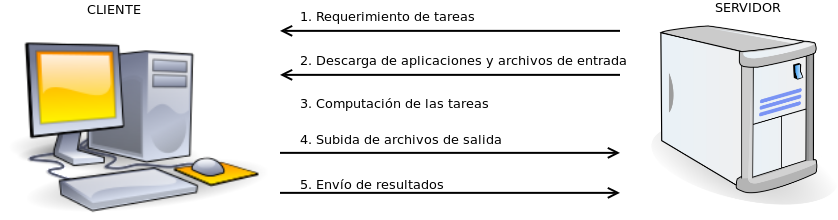
\includegraphics[scale=0.45]{images/how-boinc-works.png}
		\caption{Interacción entre cliente y servidor}
		\label{fig:how-boinc-works}
		\end{center}
\end{figure} 

El requerimiento que un cliente envía al servidor para solicitar trabajos consiste de un archivo XML en donde se detalla toda la información de hardware, de disponibilidad y a su vez se incluye el requerimiento de nuevos trabajos. En el caso de que se hayan completados trabajos, también se incluye la lista de dichos trabajos. 

Cuando el servidor responde el requerimiento, envía al cliente un mensaje de que incluye una lista de nuevos trabajos especificados mediante un elemento XML que lista la aplicación, los archivos de entrada y salida, y un conjunto de servidores desde dónde cada archivo puede ser descargado.

\subsection{Entrega de créditos}

El servidor del proyecto mantiene un registro sobre cuántos trabajos ha computado cada cliente; este registro es llamado \textit{créditos}. Básicamente según la cantidad de trabajo que ha realizado el cliente el servidor le otorga una cierta cantidad de créditos como bonificación.

La mayoría de los proyectos BOINC manejan el sistema de créditos de la siguiente manera:

\begin{itemize}
\item Cada tarea puede ser enviada a dos o más computadoras. El proyecto hace esto para comparar los resultados de cada tarea y verificar que no se estén enviando resultados erróneos.
\item Cuando los clientes reportan los resultados, estos reclaman cierto monto de créditos basado en la cantidad de tiempo de CPU que fue utilizado para procesar el trabajo
\item Cuando al menos dos resultados fueron reportados, el servidor los compara y si éstos se corresponden se le asigna a cada usuario el mínimo monto de créditos reclamado por alguno de ellos.
\end{itemize}

\subsubsection{Créditos vía Trickle Messages}

Los Trickle Mesagges permiten que las aplicaciones puedan comunicarse con el scheduler durante la ejecución de una workunit. Éstos pueden ir en cualquier dirección: los Trickle-Up son mensajes que van desde la aplicación cliente al scheduler y los Trickle-Down son los que toman el sentido contrario.

Este mecanismo tiene los siguientes usos:\\

Para solicitar créditos parciales:
\begin{itemize}
\item La aplicación cliente envía un mensaje trickle-up conteniendo su actual uso de CPU, así el usuario puede obtener créditos parciales.
\item El scheduler envía un mensaje Trickle-Down conteniendo el crédito total que posee hasta el momento el usuario.
\end{itemize}

Para verificar estado:

\begin{itemize}
\item La aplicación cliente envía un mensaje trickle-up conteniendo un resumen de su estado de ejecución, así el scheduler puede decidir si la computación debe ser abortada o debe continuar.
\item El scheduler envía un mensaje Trickle-Down diciéndole a la aplicación que aborte.
\end{itemize}

\subsection{Demonios de BOINC}

En el contexto de la informática, un demonio es un programa que realiza cierta tarea específica y se ejecuta en segundo plano, en lugar de estar bajo el control directo del usuario. 

En el caso de BOINC, los demonios son programas que forman parte del servidor y cumplen con diferentes roles dentro del proyecto.

\subsubsection{Demonios para el manejo de trabajos}

El manejo y distribución de trabajos en un proyecto BOINC incluye ciertos demonios los cuales son independientes de la aplicación que se esté ejecutando.

\textbf{\\Work Generator}: es uno de los componentes del núcleo del sistema BOINC. Está diseñado para crear workunits y results que se emitirán a los participantes para ser procesados. Su tarea consiste en crear los trabajos y organizar sus archivos de entrada para luego enviarlos a los clientes.

\textbf{\\Feeder}: mantiene una conexión directa con la base de datos y se encarga de crear un segmento de memoria compartida utilizado para transferir registros de la base de datos al scheduler.
 
Cuando un cliente realiza una conexión con el scheduler, este demonio se encarga de aislar al scheduler de la base de datos y conectarlo a esta última. De esta manera se le quita al scheduler la carga de mantener una conexión directa con la base de datos.

\textbf{\\Transitioner}: su función es manejar los estados de transición de las workunits y results. Se encarga de verificar continuamente si las workunits están listas para ser enviadas o si algún result fue recibido.
Cuando una workunit es creada, el transitioner se encarga de crear los results iniciales en la tabla result para dicha workunit. Si la ejecución de la workunit falla, este demonio creará nuevos results para reintentar la ejecución. Cuando los resultados son enviados nuevamente al servidor, el transitioner los toma para actualizar el estado de los mismo en la base de datos. Luego de actualizar su estado, este demonio crea un conjunto de resultados que son marcados como “listos para validar” que luego serán tomados por el demonio Validator.

\subsubsection{Demonios para el manejo de resultados}
\label{seccion:demonio:validator}
\textbf{\\Validator}: como el nombre lo indica, este demonio se encarga de hacer la validación de los resultados enviados por los clientes para determinar si son correctos o no. Se debe tener un validator por cada aplicación que se vaya a ejecutar en el proyecto. Este demonio solo va a considerar resultados correspondientes a aquellas unidades de trabajo cuyo flag \texttt{NEED\_VALIDATE} esté activo. 

Además, es el encargado de asignar créditos a los usuarios por sus trabajos realizados.

Luego de que los resultados de una workunit pasan por este demonio, de todos ellos se obtiene un solo resultado válido denominado \textit{resultado canónico}.

\textbf{\\Assimilator}\label{boinc:assimilator}: este demonio se encarga de tomar los trabajos completados para realizar determinadas tareas luego de que el demonio Validator determine si encontró el resultado Canónico para una workunit, o bien la marcó como errónea. 

Las tareas a realizar por el assimilator suelen ser específicas de la aplicación. Para workunits validadas correctamente, estas tareas podrían consistir en copiar los archivos de salida desde el directorio “upload” a otro directorio permanente, o llegar a analizar el archivo de salida y registrar nueva información en la base de datos, o bien generar nuevas workunits. Para workunits erróneas, generalmente se genera una salida en un archivo informando el error.

\subsubsection{Demonios para la limpieza del proyecto}

\textbf{\\File Deleter}: es el encargado de limpiar todos los archivos de workunits y results que el proyecto ya no necesita. Básicamente se encarga de eliminar los archivos de los directorios upload y download que fueron utilizados para realizar determinadas tareas que ya cumplieron su ciclo y fueron finalizadas. 

\textbf{\\Database Purge}: este demonio se encarga de eliminar los registros de la base de datos para mantenerla lo más pequeña posible y así no alterar el rendimiento de las consultas.

Si consideramos la manera en que el proyecto trabaja, el tamaño de las tablas de workunit y results se incrementa significativamente. Para evitar que ésto ocurra, BOINC provee el demonio \texttt{db\_purge} el cual mueve los registros de las tablas workunit y result a un archivo XML que será almacenado en el directorio \texttt{archive/} creado por el mismo demonio. Los registros de la tabla workunit son eliminados solo cuando sus archivos de entrada hayan sido eliminados.


\section{FuD}
\label{seccion:fud}

\subsection{¿Qué es FuD?}

FuD es un framework para automatizar la implementación de aplicaciones distribuidas. El uso de FuD no depende del problema que se quiera implementar y tampoco 
obliga a utilizar un modelo de comunicación en particular. Por consiguiente, las aplicaciones FuD pueden correr en clústers heterogéneos y dinámicos. 
Es decir, que el procesamiento en los clientes puede variar de acuerdo al hardware y software con el que se cuente. Por ejemplo, uno podría contar con muchas 
combinaciones de sistemas operativos y arquitecturas de hardware corriendo simultáneamente, además, el hecho de que el clúster sea dinámico significa que el procesamiento
 de los clientes puede fallar en un momento dado, que su disponibilidad no es fiable y que incluso pueden desconectarse sin previo aviso o bien, nuevos clientes pueden
 conectarse durante la ejecución de la aplicación.

En sí, FuD es sólo una implementación parcial de una librería si el middleware de distribución por defecto, \textit{boost::asio}, es quitado. Sin embargo, este middleware se
 incluye con la distribución de FuD y por lo tanto el framework puede compilarse como una librería. Una versión compilada de FuD consta de una librería para la distribución de
 trabajos utilizando un middleware de distribución en particular. Las librerías que surjan de compilar con diferentes middlewares de distribución deberían funcionar sin problemas,
 siempre y cuando la disponibilidad de clientes no sea un problema para algún middleware. Esto último significa que el mismo problema puede ser resuelto en diversos clústers de ordenadores, hasta en una simple computadora ejecutando la aplicación cliente y servidora juntas.

Es importante tener en cuenta que las diferentes implementaciones de middleware deberían beneficiar a los clústers que cuenten con el mismo diseño 
para el cual el middleware fue diseñado. Por ejemplo, MPI es más adecuado para clústers de ordenadores interconectados localmente mediante una vía rápida.
 Por el contrario, BOINC ofrece una capacidad de procesamiento mucho mayor a pesar de aumentar el costo de comunicación vía Internet.
Organizaciones sin fines de lucro en la mayor parte de los casos no disponen de grandes capacidades de procesamiento y por lo que generalmente dependen de
 los diferentes tipos de contribuciones recibidas para así poder manejar sus necesidades computacionales.


\subsection{¿Cómo funciona una aplicación FuD?}

En su sentido más amplio, FuD se divide en dos aplicaciones: el servidor y el cliente. Para cualquier proyecto FuD, debe existir exactamente 
un servidor con uno o varios clientes conectados a él. 

El servidor y sus clientes mantienen una relación master-worker por lo que el servidor es 
el encargado del progreso general del sistema y los workers (clientes) son los encargados de realizar el procesamiento de datos.

\subsubsection{Clientes de procesamiento}

Un cliente de procesamientos, conocido en FuD como \texttt{ClientProcessor}, es un nodo de procesamiento conectado al servidor.
 Los clientes de procesamiento pueden tomar muchas formas y tener capacidades de cómputos muy diferentes, por lo que no deben hacerse
 suposiciones de cuán rápido un cliente puede resolver un trabajo, de su disponibilidad o de cualquier otra característica.

La única tarea de un cliente de procesamiento es esperar por un mensaje proveniente desde el servidor el cual contendrá encapsulado 
algún trabajo que necesita ser realizado. 

Cada cliente de FuD es independiente de los demás clientes, por lo que desconoce cómo afectará este trabajo al resto del sistema.
Cuando el cliente recibe un mensaje desde el servidor, éste debe procesarlo y una vez finalizado debe informa el resultado obtenido de la computación al servidor.
La figura \ref{fig:Client-Server} muestra un servidor corriendo una aplicación llamada The clusterer que utiliza la librería FuD con la implementación asincrónica de E/S (\texttt{ASIO}\footnote{Asio es una librería de código abierto, desarrollada en C++ para la comunicación en red. Ésta provee a los desarrolladores un consistente modelo de E/S asincrónico utilizando el enfoque moderno de C++.}) perteneciente a la librería \texttt{Boost} para manejar las conexiones de la capa de comunicación del framework.

\begin{figure}[H]
\begin{center}
  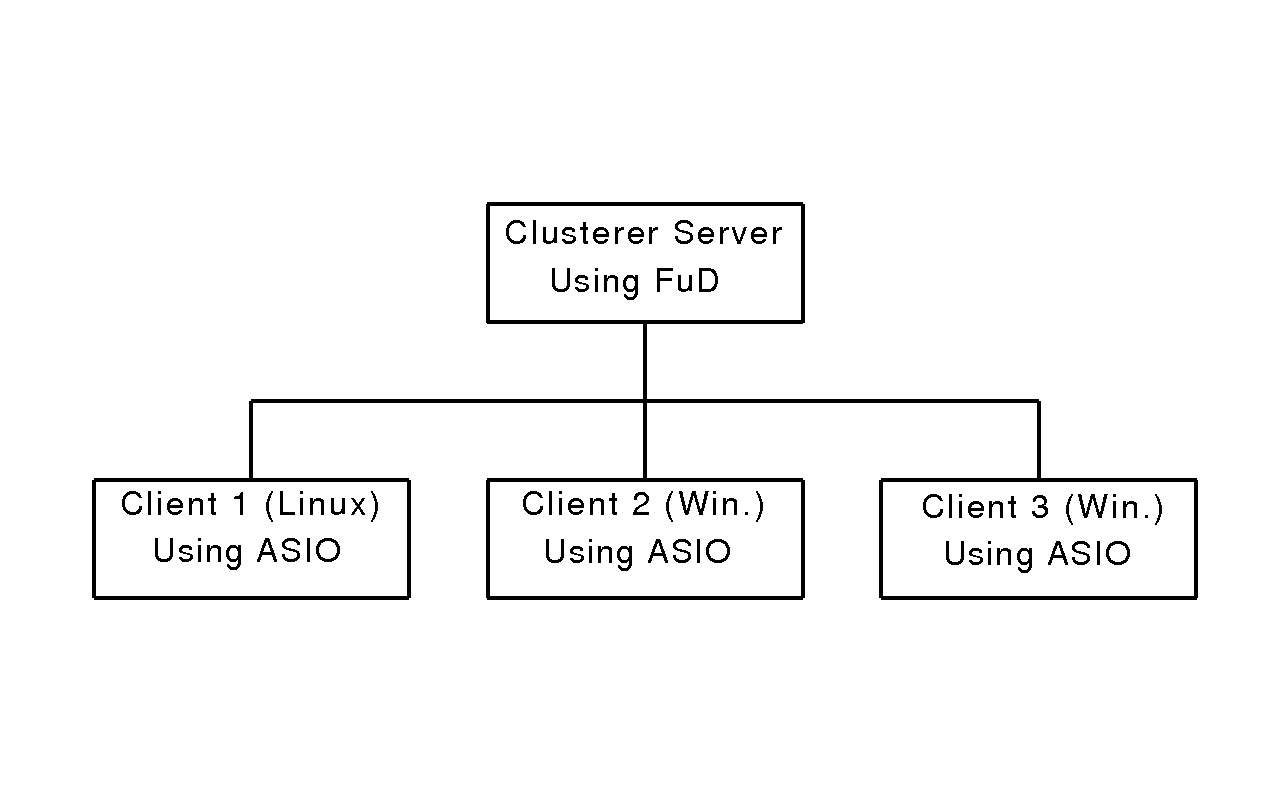
\includegraphics[height=3.5in,width=5.0in]{images/FuD-fig1.png}
\caption{Muestra tres clientes conectados al servidor}
\label{fig:Client-Server}
\end{center}
\end{figure} 

En este caso, hay dos tipos de sistemas operativos diferentes conectados al servidor.

\subsubsection{Trabajos distribuidos}

Un \texttt{DistributableJob} es un concepto de trabajo abstracto que encapsula cualquier trabajo que será realizado. No existe un límite para la cantidad y tipos
 de trabajos distribuibles que pueden ser creados. 

Es posible que un proyecto complejo requiera de diferentes tipos de trabajos distribuibles,
 donde cada uno de ellos tendrán varias instancias para diferentes casos.

La propiedad más importante de estos trabajos a gran escala es que ellos pueden ser subdivididos en tareas más pequeñas llamadas \texttt{JobUnits},
 donde cada una de ellas representa una computación concreta que será llevada a cabo por alguno de los nodos de procesamiento.

Las \texttt{JobUnits} generadas por un \texttt{DistributableJob} tienen dos características importantes:
\begin{enumerate}
 \item  A pesar que la generación se da en un orden determinado, no debe ser un requerimiento el orden en cómo las job units son computadas.
\item  Dos \texttt{JobUnits} no deben representar la misma computación.
\end{enumerate}

Por lo tanto, la relación entre trabajo distribuible y unidad de trabajo es que este último es una sub-tarea del primero. Solo existen dos niveles de subdivisión 
por lo que una job unit no puede ser sub-dividida en tareas más pequeñas. Considerar el ejemplo de la figura \ref{fig:example} donde se muestra cómo se puede construir una aplicación
 para realizar la sumatoria de la suma de N vectores. Supóngase que  se tienen vectores de 1 hasta N donde cada uno tiene una cantidad variable de elementos y se quiere calcular
 la sumatoria de la suma de todos los elementos en cada vector.

  Es fácil ver que solo se necesita de un solo trabajo distribuible: uno que pueda llevar a cabo la suma de los elementos
 de un vector. Luego, este mismo \texttt{DistributableJob} es re usado para calcular la suma de los resultados parciales obtenidos y almacenados en el vector temporal T.

Es importante destacar que aquí existen diversas posibilidades de sincronización, pero aquí elegimos una simple:

\begin{enumerate}
 \item  Los pasos 1 y 2 se ejecutarán de manera concurrente. En cualquier momento dado, todos los clientes conectados podrían estar procesando secciones diferentes de diferentes vectores.
\item El paso 3 se realizará una vez que los \texttt{DistributableJobs} de 1 a N estén completos. En este punto, el vector T contendrá los resultados parciales necesarios para llevar
 a cabo la suma del último vector. Por lo tanto, en ese momento se crea un nuevo trabajo distribuible N+1 el cual resuelve la sumatoria de todos los elementos de T. Cuando
 este \texttt{DistributableJobs} finalice, habremos obtenido la suma total de todos los vectores disponibles.
\end{enumerate}


\begin{figure}[H]
\begin{center}
  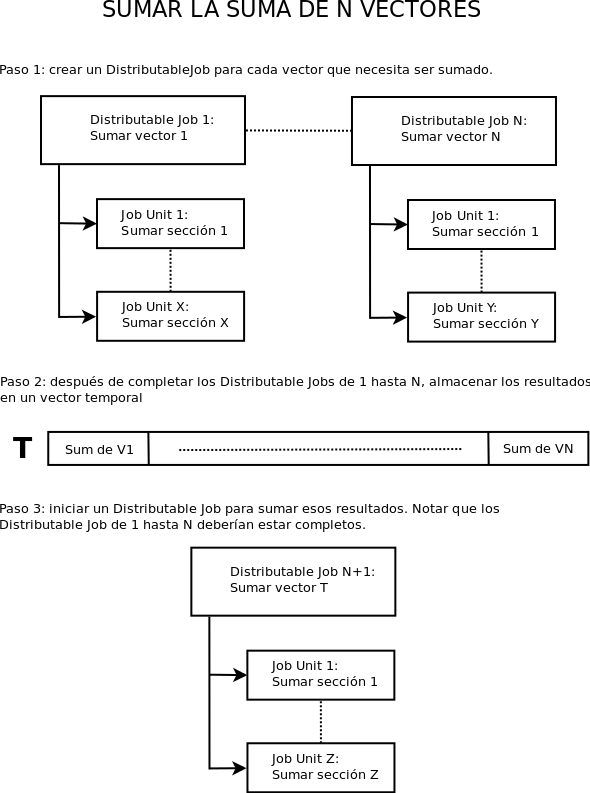
\includegraphics[height=7.5in,width=5.0in]{images/FuD-fig2.png}
\caption{Muestra el proceso de sumar N vectores}
\label{fig:example}
\end{center}
\end{figure} 


\subsubsection{Unidades de Trabajo}

Una \texttt{JobUnit} es un trabajo abstracto que encapsula el concepto de una tarea simple que será realizada. 
Una \texttt{JobUnit} es atómica por lo que no puede subdividirse en otras unidades de trabajo. La tarea en sí debe ser representada por un mensaje,
 el cual será pasado a un cliente de procesamiento quien se encargará de computarla.
Una característica importante de las \texttt{JobUnits} es su tamaño. Existen dos maneras de observar su tamaño: uno es el definido por el problema de la aplicación,
y el otro es el tamaño en bytes del mensaje que lleva.

Los tamaños de las \texttt{JobUnits} pueden variar por muchas razones, sin embargo es importante considerar algunas reglas en su generación:
\begin{enumerate}
\item Su tamaño en bytes no debería ser muy grande ya que podría obstruir un canal de comunicación utilizado.
\item  El tamaño del problema no debería ser muy grande de lo contrario los clientes de procesamiento podrían necesitar una cantidad de tiempo irrazonable para resolver la tarea.
\item  La combinación de estas dos nociones de tamaño debe darse de tal manera que el tiempo para comunicar el mensaje sea inferior al tiempo necesario para el procesamiento de la tarea. 
El objetivo de ésto es minimizar el tiempo total de computación consumido por un proyecto dado. 
\end{enumerate}

En el ejemplo dado en el diagrama de la figura \ref{fig:example} el único tipo de unidad de trabajo es el que puede sumar una serie de elementos.
 En este caso, el mensaje será una secuencia numérica en sí y el mensaje de retorno será un simple número que representará el resultado de la suma de esa sección.
En el caso del diagrama de la figura \ref{fig:example}, un vector pequeño podría producir solamente una simple \texttt{JobUnit} que encapsule la suma del vector entero.

\subsubsection{Manejador de Clientes}

El \textit{ClientsManager} es el modulo encargado de manejar la registración y disponibilidad de clientes de procesamiento. La figura \ref{fig:Client-Server}
 muestra un posible estado del modulo donde hay 3 clientes de procesamiento conectados. El manejador de clientes puede tener diferentes implementaciones que se adapten a diferentes diseños de clústers.\\
Por defecto, FuD se provee con la implementación asincrónica de E/S (\textit{ASIO}) de Boost para manejar las conexiones de la capa de comunicación del framework.
El propósito de esta tesis es proveer de una nueva implementación de este modulo que permita a las aplicaciones desarrolladas con FuD
 entrar en el mundo de la computación distribuida y voluntaria brindada por BOINC.

\subsubsection{Manejador de Trabajos}

El eje central para la gestión de \texttt{DistributableJobs} y \texttt{JobUnits} de la aplicación servidora es el \texttt{JobManager}. Éste es el encargado de
 administrar estos dos tipos de trabajos al mismo tiempo que mantiene comunicaciones con el \texttt{ClientsManager} con el fin de maximizar el uso de los recursos disponibles en un momento dado.

\subsubsection{La aplicación principal}

Para unificar todos estos conceptos, el desarrollador de la aplicación debe implementar instancias de \texttt{DistributableJob} y utilizarlas en la aplicación principal.

\subsection{Diseño de FuD}

Como se mencionó al comienzo de esta sección, el diseño de FuD se divide en dos partes, cliente y servidor donde cada una de ellas se encuentra organizada en
 tres capas bien definidas. Cada una de ellas tiene una funcionalidad clara y específica.

La comunicación entre las capas es estrictamente limitada ya que existe un solo punto de comunicación con la capa del anterior o del siguiente nivel.

Cuando un mensaje es creado, éste debe atravesar las diferentes capas comenzando desde la de nivel más alto hacia la capa inferior, y luego recorrer en
 sentido contrario las capas del lado receptor. Ver la figura \ref{fig:FuD-Design}.


\begin{figure}[H]
\begin{center}
  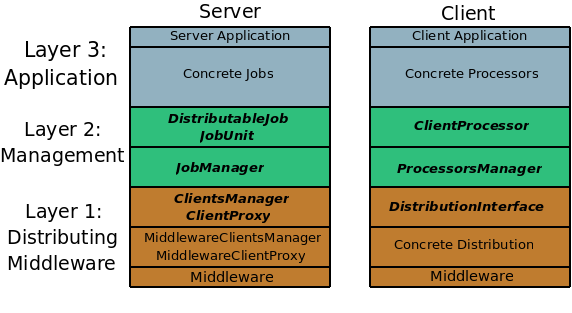
\includegraphics[height=3.5in,width=5.0in]{images/FuD-diseno.png}
\caption{Capas del framework FuD }
\label{fig:FuD-Design}
\end{center}
\end{figure} 


\subsubsection{Capa de aplicación (L3)}

Esta capa proporciona los componentes que contienen todos los aspectos del dominio del problema a resolver. Dichos aspectos incluyen todas las definiciones
 de datos y sus tratamientos correspondientes como así también todos los algoritmos relevantes para la resolución del problema en cuestión.
Por estos motivos, esta capa no es, en algún sentido, considerada como parte de FuD. La implementación de una aplicación que usa la librería,
 no es parte de la librería. Sin embargo, su inclusión es una ayuda valiosa para la comprensión de cómo funciona FuD.

Es necesario que del lado del servidor se implemente la aplicación principal, la cual hará uso de una simple interfaz en la abstracción de un trabajo distribuible permitiendo así codificar la estrategia de distribución de trabajos.
Del lado cliente, solo se necesita implementar los métodos encargados de realizar las computaciones indicadas por una unidad de trabajo.

\subsubsection{Capa de administración de trabajos (L2)}

La responsabilidad de esta capa es el manejo de trabajos, lo cual incluye la creación de instancias de \textit{DistributableJobs}
 y el pedido de generación de \texttt{JobUnits} las cuales van a ser entregadas a la capa inferior para su procesamiento. Una vez que la tarea finalice, se debe informar a las capas superiores de la tarea completada y los resultados obtenidos.

\subsubsection{Capa de distribución (L1)}

En el lado del servidor, la registración de clientes y sus estados es manejado por esta capa. 

Tanto del lado cliente como del servidor, la parte fija está dada por interfaces. Las implementaciones concretas de este nivel son variables
 y están determinadas por el middleware a utilizar, por ejemplo \textit{Boost.Asio}, \textit{MPI} o \textit{BOINC}.  

Desde esta vista abstracta de diseño, es importante destacar que la capa \textbf{L1} constituye por sí sola un particular esquema de manejo de clientes. Éste podría implementarse usando threads o procesos en un simple núcleo, una \textit{API} de memoria distribuida como \textit{MPI} o, como en el caso de esta tesis, computación voluntaria a través de internet utilizando BOINC.

Estas implementaciones separadas deberían poder intercambiarse sin ningún problema. Utilizar cualquiera de las implementaciones de esta capa no debe afectar la resolución del problema que se intenta resolver, por lo que los resultados obtenidos deben ser los mismos.
Debe notarse que en todo el sistema el tiempo total de cálculo de una unidad de trabajo en un entorno ideal está dado por varios factores:\\

T$_{job−unit}$ = T$_{send}$ + T$_{compute}$ + T$_{receive}$ + T$_{handle−results}$

\vspace{5mm}

T$_{send}$ y T$_{receive}$ dependen de la comunicación, T$_{receive}$ depende de la arquitectura del cliente y T$_{handle−results}$ depende del servidor. 

El tamaño de una unidad de trabajo debe minimizar esta ecuación. Si un usuario contara con un solo núcleo de procesamiento y por ejemplo
 usara threads las variables de tiempos T$_{send}$  y T$_{receive}$ serían nulas mientras que las dos restantes se incrementarían por el costo de mantener varios threads en ejecución.  


\section{El lenguaje de programación C++}

\textit{C++} es un lenguaje de programación desarrollado en el año \textit{1979} por \textsc{Bjarne Stroustrup} en los laboratorios \textsc{Bell}. 
Inicialmente era llamado \textit{“C con clases”} ya que se presentaba como una mejora o extensión del lenguaje de programación \textit{C}. 
Los contenidos más completos sobre este lenguaje se los pueden encontrar en el propio libro de Bjarne Stroustrup \cite{cplusplus}.\\

\textit{C++} es un lenguaje multi-paradigma y estáticamente tipado. Es considerado un lenguaje de nivel medio, ya que comprende características de lenguajes de alto y bajo nivel.\\

Este lenguaje fue elegido como lenguaje de implementación del framework FuD ya que éste permite el uso de técnicas orientadas a objetos y produce eficiente código assembler.
 Este lenguaje también ofrece una gran cantidad de librerías para facilitar la resolución de determinados problemas, permitiendo al programador concentrarse en dichos problemas
 y no en implementar tipos de datos abstractos ya conocidos.

Para nuestro proyecto hicimos uso del lenguaje \textit{C++}, ya que debimos implementar nuevos módulos para la capa de distribución del framework FuD e integrar
 funciones y variables del middleware BOINC las cuales fueron implementadas en el lenguaje \textit{C}.

		\chapter{Metodología de trabajo}
\label{chapter:metodologia}

\section{Prácticas de software}

Para el desarrollo de este proyecto se optó por utilizar una metodología de trabajo basada en las buenas prácticas de software establecidas en el artículo publicado por IBM \textit{Best practices for software development projects} \footnote{\url{http://www.ibm.com/developerworks/websphere/library/techarticles/0306_perks/perks2.html}}. De las prácticas mencionadas en este artículo, las siguientes fueron implementadas satisfactoriamente:

\subsection{Captura de requisitos}

Reunir y acordar los requerimientos es una etapa fundamental para el éxito de un proyecto. Esto no implica necesariamente que todos los requerimientos deban ser corregidos antes de que el diseño y codificación sean efectuados, pero es importante que el equipo de desarrollo entienda qué necesita construir.

Para comenzar con el desarrollo de FuD-BOINC, dedicamos un tiempo considerable en comprender las necesidades que la organización FuDePAN\footnote{\url{http://fudepan.org.ar/}} deseaba cubrir con nuestro proyecto. 

\subsection{Diseño}

Aún con una buena arquitectura es posible tener un mal diseño. Los dos principios básicos aquí son ``mantener la simplicidad'' y ``ocultar la información''. En muchos proyectos es importante llevar a cabo un Análisis y Diseño Orientado a Objetos usando UML \footnote{\url{http://www.uml.org/}}.

Debido a las características del problema planteado para el desarrollo de este proyecto y considerando que FuD ya provee de un diseño que permite contar con varias implementaciones de su capa de distribución, nuestra labor en esta etapa fue, en un principio, entender su diseño e investigar la arquitectura de BOINC para luego rediseñar las partes que iban a ser afectadas por nuestra implementación.

\subsection{Construcción de código}

Sin duda, una importante etapa del desarrollo fue la construcción del código fuente. Para ello fue necesario disponer de una aplicación ``juguete'' que utilizara a FuD en su implementación y que nos permitiera corroborar el funcionamiento de FuD con el middleware BOINC. En este contexto fue que se decidió utilizar la aplicación ejemplo \textit{Counter} provista por el framework.

Cada cambio realizado en el código, por más mínimo que fuera, fue debidamente testeado en su entorno final para corroborar que su funcionamiento y adaptación con el proyecto BOINC fuesen el esperado.

\subsection{Testing}

El testing es una parte importante de todo proceso de desarrollo de software. En nuestro caso, se utilizaron las aplicaciones de ejemplo que el framework ofrece para probar diferentes características o secciones de nuestro proyecto. Dichas pruebas permitieron determinar varias fallas o errores que debieron ser corregidos para el correcto funcionamiento de las aplicaciones.  

\subsection{Gestión de la configuración}

La gestión de la configuración consiste en conocer el estado de todos los artefactos de que componen el sistema o proyecto, gestionar el estado de esos artefactos, y la liberación de diferentes versiones de un sistema

\subsection{Control de calidad y defectos}

A medida que el proyecto se codifica y se prueban las funcionalidades involucradas en cada revisión, los defectos encontrados, con sus respectivas soluciones, ayudan a medir la madurez del código. Por ello, es importante utilizar un sistema de seguimientos de errores que esté conectado con el sistema de control de versiones.


\section{Gestión de la configuración}

Cuando se construye software de computadora, los cambios son inevitables. Además, cada cambio puede aumentar el grado de confusión entre los participantes que se encuentren trabajando en el proyecto. La confusión surge cuando no se han analizado los cambios antes de realizarlos, no se han registrado antes de implementarlos, no se les han comunicado a aquellas personas que necesitan saberlo o no se han controlado de manera que mejoren la calidad y reduzcan los errores.

En este contexto, para desarrollar \textit{FuD-BOINC}, fue necesario llevar el estado de cada elemento del software: código fuente, diagramas, archivos de configuración, etc. Se utilizó entonces un repositorio \textbf{svn} alojado en \textbf{googlecode} que nos permitió controlar cada cambio realizado sobre cada elemento del software. 

Información sobre subversion (svn) y sus características pueden ser encontradas en el libro de O'Reilly's\cite{svn}. Información sobre el uso de \textbf{googlecode} puede ser consultada en su sitio web\footnote{\url{http://code.google.com/projecthosting/}}.


\section{Seguimiento de errores}

A lo largo de todo el proceso fue necesario hacer diversos seguimientos de errores, tanto de este proyecto como así también de proyectos y librerías importantes para la aplicación Parallel Clusterer\ref{seccion:pruebas:clusterer}

Todos los errores, defectos y cambios sobre el proyecto, e inclusive sobre los proyectos externos utilizados, fueron reportados usando el issue tracker de googlecode\footnote{\url{http://code.google.com/p/support/wiki/IssueTrackerAPI/}} mediante el cual se pudo hacer un seguimiento de cada detalle informado. 

Para dudas o consultas referidas a los proyectos mencionados anteriormente, se utilizaron diversos medios de comunicación que la misma fundación provee y que permitieron contactarnos directamente con los desarrolladores del proyecto. Para tal fin, se utilizó un grupo de discusión y un canal de chat, ambos integrados por todos los miembros de FuDePAN\footnote{\url{http://www.fudepan.org.ar/}}.


\section{Herramientas}

\subsection{GNU/Linux y Software Libre}

Es un sistema operativo basado en GNU/Linux que está conformado por varios componente, entre ellos el núcleo Linux y los programas desarrollados por el proyecto GNU.
Linux es un sistema operativo libre del tipo Unix sobre el cual se desarrolló la mayor parte de este proyecto. Tanto este proyecto como así también la mayoría de las herramientas utilizadas a lo largo de su desarrollo se encuentran bajo la licencia \textbf{GPL} \footnote{\url{http://www.gnu.org/licenses/gpl-3.0.txt}}, siglas que provienen del inglés \textbf{\textit{General Public License}}. 

El termino ``Libre'' se refiere a la capacidad de poder analizar y modificar el código fuente de la herramienta, permitiendo redistribuir 
el trabajo sin restricción alguna, excepto que se debe mantener la licencia y la referencia a los autores originales. 

\subsection{GNU Toolchain}

Linux ofrece una serie de herramientas de gran utilidad para desarrolladores, de las cuales varias fueron utilizadas para el desarrollo de este proyecto:

\begin{itemize}
\item \textbf{GCC ( GNU Compiler Collection )}: es un conjunto de compiladores creados por el proyecto GNU. Es software libre y distribuido bajo la licencia GPL. 
Originalmente GCC significaba GNU C Compiler (compilador GNU para C), porque sólo compilaba el lenguaje \textit{C}. Posteriormente se extendió para compilar \textit{C++}, \textit{Fortran}, \textit{Ada} y otros.

\item \textbf{GDB ( The GNU Project Debbuger )}: es el depurador estándar desarrollado para  sistema operativo GNU. Es un depurador portable que se puede utilizar en varias plataformas Unix y funciona para varios lenguajes de programación como C, C++ y Fortran.

\item \textbf{CMake}\label{tool:cmake}: el nombre viene de la abreviatura Cross Platform Make\footnote{\url{http://www.cmake.org/}}. Es una herramienta multiplataforma y de código abierto utilizada para la generación o automatización de código. 
Fue diseñado para soportar jerarquía de directorios y aplicaciones que dependen de múltiples librerías. 

\item \textbf{\LaTeX}: es una herramienta para la composición de textos y está orientada especialmente a la creación de libros,
 documentos científicos y técnicos que contengan fórmulas matemáticas. También es muy utilizado para la composición de artículos académicos,
 tesis y libros técnicos, dado que la calidad tipográfica de los documentos realizados con LaTeX es comparable a la de una editorial científica de primera línea.

\item \textbf{Edición}
\begin{description}
 \item \textbf{Gedit}: es el editor de textos predeterminado de GNOME. Básicamente es un editor de textos de propósito general, 
 cuyo diseño se enfatizó en la simplicidad y facilidad de  uso. Incluye herramientas para la edición de código fuentes,
 textos estructurados y lenguajes de marcado. Este es compatible con UTF-8 para GNU/Linux, Mac OS X y Microsoft Windows
\item \textbf{Texmaker / Kile}: editores de Tex/LaTeX utilizados para la documentación de este proyecto.

\end{description}

\item \textbf{Gráficos}

\begin{description}

\item \textbf{Bouml}: editor de diagramas \textbf{\textit{UML}}. Más información en \url{http://bouml.free.fr/}
\item \textbf{Día}: editor de diagramas de propósito general. Más información en \url{http://live.gnome.org/Dia/}.

\end{description}

\item \textbf{Documentación de código}

\begin{description}
 \item \textbf{Doxygen}: es un generador de documentación para código fuente. Se aplica en los lenguajes \textit{C}, \textit{C++}, \textit{Java}, \textit{Objective-C} entre otros.
\end{description}

\item \textbf{Análisis estático de código}

\begin{description}

 \item \textbf{Cloc}: es un programa desarrollado en Perl para contar la cantidad de líneas de código  de un sistema. Cuenta líneas en blanco, líneas de comentarios y líneas de código fuente.

\item \textbf{CCCC}: herramienta para el análisis de los archivos fuentes “\textit{.cpp}”. Esta genera reportes y genera un informe sobre diversas métricas del código. 

\item \textbf{GCov}: es una herramienta que se utiliza en conjunción con \textit{GCC} para hacer pruebas de cobertura de código de un programa. 
Su tarea consiste en informar cuantas veces se ejecuta un línea de código, que línea de código se ejecuta actualmente y cuánto tiempo de computación usa cada sección de código.
Esta herramienta es útil por ejemplo para encontrar ciertas líneas de código que no se utilizan.

\end{description}
\end{itemize}

\subsection{Aplicaciones BOINC}

Para la creación del proyecto BOINC sobre el cual se ejecutó la aplicación servidor compilada con FuD utilizando el middleware BOINC
 se utilizó el script \textbf{\textit{make\_project}} que ofrece BOINC en su código fuente. 

Para participar como clientes de nuestro proyecto \textit{BOINC} utilizamos las aplicaciones cliente \textit{BOINC-Client} y \textit{BOINC-Clients-manager}.
Dichas aplicaciones se pueden descargar de la página \url{http://boinc.berkeley.edu/download_all.php}

Tanto el Script como las aplicaciones cliente fueron explicadas en la sección \textbf{\textit{2.5.BOINC}} de este documento.


\subsection{Microsoft Windows}

Para este proyecto se realizó la compilación del lado cliente de ciertas aplicaciones utilizando la herramienta \textit{Visual Studio} 
desarrollado por Microsoft para los  sistemas operativos \textit{Microsoft Windows}. 

\vspace{0.5cm}

\begin{description}

 \item \textbf{Visual Studio}

Microsoft Visual Studio soporta varios lenguajes de programación tales como \texttt{Visual C++}, \texttt{Visual C\#}, \texttt{Visual J\#}, 
\texttt{ASP.NET} y \texttt{Visual Basic .NET} y actualmente desarrollaron extensiones para dar soporte a otros lenguajes.

Visual Studio permite a los desarrolladores crear aplicaciones, sitios y aplicaciones web, así como servicios web en
 cualquier entorno que soporte la plataforma \texttt{.NET} (versión 2002 o superior) . 

Para la compilación de las aplicaciones cliente se utilizo el Visual Studio 2005 Express Edition. La edición express ha sido diseñada para principiantes, aficionados y pequeños negocios, 
siendo esta gratuita. Las ediciones Express carecen de algunas herramientas avanzadas de programación así como de opciones de extensibilidad.\\
Esta edición, está disponible en la página \url{http://msdn.microsoft.com/es-es/express/aa975050}. 

\end{description}

\vspace{0.4cm}

Para obtener ciertas librerías necesarias desde repositorios \textbf{SVN} y \textbf{Mercurial} respectivamente, se utilizaron las siguientes herramientas:

\begin{description}
 \item \textbf{TortoiseSVN}
TortoiseSVN es un cliente de Subversion implementado como extensión para el Shell de Windows. Es software libre liberado bajo la licencia GNU GPL. Más información en \url{http://tortoisesvn.net/}

\item \textbf{TortoiseHg}
TortoiseHG es un cliente del control de versiones Mercurial, implementado como una extensión para el Shell de Windows. 
También incluye extensiones para GNOME/Nautilus. Más información en \url{http://tortoisehg.bitbucket.org/}

\end{description}
	
	\part{Capa de distribución FuD-BOINC}\label{BOINC}
		\chapter{Sobre FuD-BOINC}
\label{chapter:sobre:fud:boinc}


\section{El problema}

El problema que motivó el desarrollo de esta tesis consiste en la implementación de una nueva capa de distribución del framework FuD utilizando el middleware BOINC\footnote{\url{http://boinc.berkeley.edu/}} para permitir que cualquier aplicación que use a FuD en su desarrollo pueda optar por utilizar la computación voluntaria como fuente de procesamiento.

El asunto surgió como una necesidad de la organización FuDePAN\footnote{\url{http://fudepan.org.ar/}} para poder ejecutar sobre un proyecto de computación voluntaria y distribuida cualquier aplicación implementada con la librería FuD, permitiendo así incrementar la capacidad de procesamiento utilizando ordenadores personales de todo el mundo y, por el contrario, evitar el uso de costosas súper-computadoras.

Por defecto, FuD sólo dispone de una única implementación de su capa de distribución, la cual fue desarrollada utilizando la librería Boost::ASIO\footnote{\url{http://www.boost.org/doc/libs/1_48_0/doc/html/boost_asio.html}} para la comunicación en red. Por ello, el objetivo principal de este proyecto es el de proporcionar una nueva implementación para dicha capa de tal manera que, al momento de desarrollar una aplicación utilizando a FuD, el desarrollador pueda elegir con qué implementación desea que su aplicación trabaje, acorde al dominio del problema que se intente resolver.

\section{Metas del proyecto}

Como se mencionó anteriormente, el objetivo principal de este proyecto fue permitir a desarrolladores de aplicaciones FuD la posibilidad de que sus ejecutables realicen computación distribuida mediante la arquitectura BOINC sin tener los conocimientos previos necesarios sobre desarrollo de aplicaciones BOINC. 

En consecuencia, se pretende brindar, a la organización FuDePAN, una noción general sobre la creación y administración de un proyecto servidor BOINC en el cual se puedan poner en funcionamiento las aplicaciones creadas con esta nueva capa de distribución.

De esta manera, FuDePAN podría dar un paso hacia adelante en lo que respecta a computación voluntaria evitando así tener que realizar importantes inversiones económicas para la adquisición de grandes nodos de procesamiento. Cabe destacar que FuDePAN es una organización sin fines de lucro por lo que sus ingresos monetarios dependen directamente de las colaboraciones que pueda percibir de diferentes organismos.

La última meta que pretende este proyecto es la de poder generar un binario de la aplicación cliente Parallel-Clusterer\footnote{\url{http://code.google.com/p/parallel-clusterer/}}, utilizando a FuD-BOINC como capa de distribución, que sea compatible con sistemas operativos Windows, ya que actualmente esta aplicación solo está disponible para Linux. El motivo de esto es claro: la mayoría de los usuarios de computadoras utilizan una versión de este sistema operativo.

\section{Tareas de investigación}

Debido a que al comienzo del proyecto desconocíamos qué era BOINC y cómo trabajaba FuD debimos realizar diversas trabajos de investigación que nos permitieron conocer aún más el dominio del problema.

A continuación se describen las tareas que se llevaron a cabo a lo largo del proyecto:

\begin{itemize}
\item Se analizó el funcionamiento general del framework FuD, focalizándonos puntualmente en la capa de distribución, el manejador de trabajos y su manejador de clientes. Aquí fue necesario conocer el diseño de la librería en conjunto con algunos puntos concretos de su implementación, verificando qué clases estaban involucradas en las tareas de comunicación y distribución de trabajos entre Cliente-Servidor. Para concluir, efectuamos la ejecución de sus aplicaciones ejemplos incluidas en el framework al mismo tiempo que analizábamos su código.
\item Se investigó cómo trabaja la arquitectura BOINC desde su forma más general hasta los detalles mínimos de implementación relacionados directamente con el dominio de nuestro problema. Se optó por usar esta postura debido a que BOINC es muy amplio y muchas de sus características no están relacionadas con el desarrollo de esta tesis, sino más bien con trabajos a futuro. Durante esta tarea se inspeccionó el código fuente de algunas de sus aplicaciones ejemplo, estudiando su estructuras y funciones tanto del lado servidor como del lado cliente.
\item Se examinó en detalle el proceso de creación y administración de un proyecto BOINC para posteriormente instalar nuestro propio proyecto. Esta tarea fue una etapa importante debido a que todo el proceso está íntimamente relacionado con la administración y configuración de un servidor web, cosa que en ese entonces desconocíamos por completo. Por este motivo, fue necesario estudiar el proceso general de instalación y configuración mencionado como así también la configuración de diversas herramientas en el ordenador servidor como fueron por ejemplo Apache, MySQL, PHP, entre otros.
\item Luego del punto anterior, fue necesario conocer la función de cada uno de los demonios que corren en un proyecto BOINC y cuál es el rol de cada uno en la interacción cliente-servidor.
\item Una vez instalado y configurado nuestro proyecto BOINC iniciamos pruebas funcionales de sus aplicaciones ejemplos al mismo tiempo que observamos detenidamente las interacciones generadas entre el servidor del proyecto y los clientes adheridos al mismo.
\item Para la compilación de las aplicaciones ejemplos de BOINC, y teniendo en cuenta que íbamos a necesitar compilar FuD con BOINC, se examinó atentamente los archivos y librerías necesarias de BOINC que permitían compilar dichas aplicaciones.
\end{itemize}

Cada una de estas tareas fueron cruciales para comprender el funcionamiento y los modos de operación tanto de FuD como de BOINC, por ello, además de su estudio al comienzo de este trabajo final, fue necesario examinar cada punto durante todo el desarrollo.

Es importante dejar en claro que todos estos puntos ocuparon un alto porcentaje del desarrollo de este proyecto; debido a nuestra falta de conocimiento y sumado a que desde la fundación también desconocían BOINC, el tiempo que nos llevó la realización de cada una de estas tareas fue bastante amplio.


\section{Cómo funciona la capa de distribución}

La capa de distribución del framework FuD está compuesta por una arquitectura del tipo cliente servidor. Ésta ofrece un modelo de computación distribuida master-worker donde el servidor actúa como master, llevando a cabo el progreso total del sistema, y los clientes actúan como worker, encargándose del procesamiento de datos.

Debido a la arquitectura utilizada por FuD y considerando que BOINC es un middleware para la computación distribuida, para el desarrollo de nuestro proyecto debimos utilizar la arquitectura cliente-servidor.

\subsection{Servidor}

El funcionamiento del servidor de FuD-BOINC tiene como base el comportamiento del servidor FuD original, agregándole ciertas funcionalidades o características que permiten a las aplicaciones desarrolladas con las librerías FuD funcionar correctamente sobre un proyecto BOINC.

Las características principales de la capa de distribución de FuD-BOINC se resumen en las siguientes:

\begin{itemize}
\item Analizar el archivo configuración del proyecto. (\texttt{config.xml})
\item Conectar con la base de datos del proyecto.
\item Crear un \texttt{ClientProxy} el cual representará a un cliente de FuD conectado al servidor de manera permanente donde su función será la de generar trabajos de BOINC y de notificar a FuD sobre \texttt{workunits} que hayan sido completadas. Para esto último, el mismo \texttt{ClientProxy} se encarga de lanzar un thread encargado de realizar las tareas que generalmente le corresponde al demonio \texttt{assimilator} de BOINC. Para más información sobre el \texttt{assimilator} de BOINC consultar la sección \ref{boinc:assimilator}.
\item Crear un archivo binario por cada \texttt{JobUnit} de FuD liberada a la capa de distribución, el cual contendrá la información de dicha \texttt{JobUnit}.
\item Crear una \texttt{workunit} por cada \texttt{JobUnit} que se pretenda enviar a procesar utilizando como entrada el archivo generado en el punto anterior. 
\end{itemize}

\subsection{Cliente}

Al igual que el servidor, también se debió adaptar el cliente de FuD para que funcione correctamente sobre un cliente BOINC \ref{boinc:manager}. 

La función principal de la aplicación cliente de FuD-BOINC es llevar a cabo las computaciones de las tareas recibidas desde el servidor. Para ello, primero debe leer la información contenida en su archivo de entrada y traducirla a \texttt{JobUnit} para luego informar a la capa superior sobre la computación a realizar.

Una vez que la computación es completada, sus resultados son encapsulados dentro de un nuevo archivo de resultado el cual será enviado por el cliente BOINC al servidor del proyecto.

Es importante dejar en claro que el cliente de FuD corre sobre el cliente de BOINC interactuando de la siguiente manera:

\begin{enumerate}
\item Cuando BOINC Manager (\ref{boinc:manager}) se inicia, suponiendo que el usuario ya ha hecho su adhesión al proyecto, inmediatamente consulta al servidor del proyecto por la existencia de nuevos trabajos que requieran ser procesados.
\item En caso de que existan tareas, BOINC Manager se encargará de descargar aquellas que sean indicadas por el servidor del proyecto.
\item Una vez descargados estos archivos, por cada uno de ellos, BOINC Manager ejecuta la aplicación cliente de FuD pasándole como argumento el archivo con los datos de la tarea a computar.
\item Cuando el cliente de FuD finaliza genera un archivo de salida conteniendo el resultado de la computación que es tomado por BOINC Manager para luego enviárselo al servidor del proyecto al mismo tiempo que consulta por nuevos trabajos.
\end{enumerate}

\section{Dependencias externas}

FuD tiene dependencia con un par de librerías. A continuación se explican qué librerías fueron utilizadas y cómo obtenerlas.

\subsection{Mili}

Mili es una colección de pequeñas y útiles librerías desarrolladas en el lenguaje C++ por FuDePAN, compuesta únicamente por cabeceras. 
No requiere instalación para su uso y ofrece soluciones simples para problemas sencillos.

Esta biblioteca provee varias funcionalidades mediante archivos cabecera, conocidos en el ámbito de C/C++ como archivos con extensión “.h”.
Mili puede ser descargada junto con su documentación desde su repositorio \footnote{\url{http://mili.googlecode.com/}}.

Mili ha sido extensamente utilizada a lo largo del desarrollo de FuD-BOINC. Se utilizaron las funcionalidades provistas por \texttt{generic\_exception}, \texttt{binary\_stream} y \texttt{RAII}.

\begin{itemize}
\item \texttt{binary\_stream}: permite serializar diferentes tipos de datos dentro de un único objeto utilizando los operadores de stream. Hay dos maneras de utilizar esta librería:
\begin{enumerate}
\item Empaquetar datos dentro de un objeto de salida (\texttt{bostream}) utilizando el operador <<.
\item Extraer datos desde un objeto de entrada (\texttt{bistream}) utilizando el operador >>.
\end{enumerate}

\item \texttt{RAII}: esta librería ofrece una implementación de RAII\footnote{\url{http://en.wikipedia.org/wiki/Resource_Acquisition_Is_Initialization}} (Resource Acquisition Is Initialization) permitiendo aplicar RAII sobre los objetos para liberar los recursos adquiridos de manera automática cuando éstos terminan su ciclo de vida.

\item \texttt{generic\_exception}: ofrece una implementación de excepciones genéricas a partir de las cuales los desarrolladores pueden crear sus propias excepciones para problemas específicos de una manera muy simple .
\end{itemize}

\subsection{Boost}

La librería Boost es una colección de librerías de código abierto que extienden las funcionalidades del lenguaje C++. Es posible descargar Boost y acceder a su documentación desde su sitio web\footnote{\url{http://www.boost.org/}}.

Durante el desarrollo de nuestra capa de distribución hicimos uso de las librerías \texttt{Boost::thread} y \texttt{Boost::bind}:

\begin{itemize}
\item \texttt{Boost thread}: permite el uso de múltiples hilos de ejecución con datos compartidos. Provee las clases y funciones necesarias para manejar estos hilos. 
\item \texttt{Boost Bind}: es una librería que ofrece una generalización para las librerías std::bind1st() y std::bind2nd() provistas por C++. Soporta un número arbitrario de funciones de objetos, funciones, punteros a funciones, etc. y es capaz de ligar cualquier argumento a un valor especifico o ligar los argumentos de entrada con valores en diferentes posiciones.

Ejemplo:

\begin{lstlisting}[frame=shadowbox, language=c++, xleftmargin=8mm, framexleftmargin=20pt, basicstyle=\footnotesize, numberstyle=\footnotesize, backgroundcolor=\color{gris}]
bind(f,1,2)			produce f(1,2)
bind(f, _2, _1)(x, y);		produce f(y, x)
bind(g, _1, 9, _1)(x);		produce g(x, 9, x)
bind(g, _3, _3, _3)(x, y, z);	produce g(z, z, z)
bind(g, _1, _1, _1)(x, y, z);	produce g(x, x, x)
\end{lstlisting}
\end{itemize}

Estas bibliotecas fueron utilizadas para crear el asimilador de tareas requerido por BOINC.

\subsection{MySQL}

Es un sistema de gestión de bases de datos relacionales muy conocido que provee acceso multiusuario a sus bases de datos.

Un proyecto BOINC utiliza una base de datos MySQL para persistir su información en el tiempo que sea necesario por lo que el desarrollo de nuestro proyecto, se hizo uso de ciertas funcionalidades que ofrece BOINC para el acceso a la base de datos y que involucran la ejecución sentencias MySQL para tal fin.

\subsection{SSL}

SSL proporciona autenticación y privacidad de la información entre servidor y clientes sobre Internet mediante el uso de criptografía. Habitualmente, sólo el servidor es autenticado mientras que el cliente se mantiene sin autenticar.

SSL se ejecuta en una capa entre los protocolos de aplicación como HTTP, SMTP, NNTP y sobre el protocolo de transporte TCP, que forma parte de la familia de protocolos TCP/IP. En la mayoría de los casos se usa junto al protocolo HTTP para formar HTTPS. 

BOINC hace uso de este protocolo para proveer seguridad en sus proyectos por lo que tuvimos que incluir dicha librería en la compilación de una aplicación FuD-BOINC.

		\chapter{Diseño}
\label{chapter:diseno}


El diseño de software consiste en resolver un problema planificando una eficaz solución de software. Luego de establecer el propósito y las especificaciones de los requerimientos del sistema, los desarrolladores emplearán el diseño para desarrollar la mejor solución posible que permita resolver el problema eficientemente. 

En cualquier proceso de diseño existen dos fases importantes: la diversificación y la convergencia. La diversificación es la adquisición de un repertorio de alternativas, de un material primitivo de diseño: componentes, soluciones de componentes y conocimiento, todo dentro de catálogos, de libros de texto y en la mente. Durante la convergencia, el diseñador elige y combina los elementos adecuados y extraídos de este repertorio para satisfacer los objetivos del diseño, de la misma manera a como se establece en el documento de los requisitos, y de la manera en que se acordó con el cliente. La segunda fase es la eliminación gradual de cualquier configuración de componentes excepto de una en particular, y de aquí la creación del producto final.

En términos generales, lo que pretende el diseño es brindar una visión arquitectónica o estructural de la solución planteada mostrando las interrelaciones de los componentes de mayor nivel, conocido como diseño de alto nivel, y a su vez especificar en detalles los componentes de implementación y operaciones lógicas implicadas en los niveles inferiores, conocido como diseño de bajo nivel.

Desde el comienzo de esta etapa se tuvieron en cuenta los cinco principios básicos de la programación orientada a objetos, comúnmente conocido como SOLID (Single responsibility, Open-closed, Liskov substitution, Interface segregation and Dependency inversion), los cuales, siempre y cuando se respeten, permiten construir software sencillo de mantener y que puede ser extendido fácilmente.

A continuación se resumen los cinco principios mencionados:
\begin{itemize}
\item \textbf{Single Responsibility Principle (SRP)}: cada elemento, ya sean paquetes, clases, métodos e incluso bloques de código, debería tener una única razón para cambiar. Esto significa que debe tener una única responsabilidad: ocuparse de una única tarea para aumentar de esa forma la cohesión y reducir el acoplamiento.
\item \textbf{Open/Closed Principle (OCP)}: una clase debe permitir ser extendida sin necesitar ser modificada. Es decir, que todo componente debe estar abierto a nuevas funcionalidades, pero cerrado a cambios en su código. 
\item \textbf{Liskov Substitution Principle (LSP)}: los objetos de una clase deberían poder sustituirse por instancias de las clases derivadas. 
\item \textbf{Interface Segregation Principle (ISP)}: crear pequeñas interfaces específicas para los clientes. Otra forma de expresarlo es que las clases que implementen una interfaz o una clase abstracta no deberían estar obligadas a implementar métodos que no utilizan.
\item \textbf{Dependency Inversion Principle (DIP)}: las abstracciones no deben depender de los detalles, los detalles deben depender de las abstracciones.
\end{itemize}


\section{Diseño de alto nivel}

Desde el punto de vista de la ingeniería de software, el diseño de alto nivel es una etapa crucial del desarrollo de software. Sus implicaciones y deficiencias afectan directamente al proyecto a lo largo de su ciclo de vida, por lo que la toma de decisiones en esta etapa es una tarea que debe ser llevada a cabo con mucha cautela.

\subsection{Capa de distribución (L1)}

Considerando que FuD-BOINC implementa una nueva capa de distribución del framework FuD, y que éste ya cuenta con un diseño definido al igual que BOINC, para este proyecto no se tuvo que realizar un diseño de alto nivel sino que se debió adaptar a los diseños provistos por ambos frameworks. Para ello, fue muy importante enfocarse ampliamente en la captura de requerimientos para conocer en detalle las características de los frameworks involucrados, para que al llegar a esta etapa se lograra construir una solución simple y eficaz en lo que respecta a esta adaptación.

La idea principal aquí fue de ajustar esta solución de manera que no afecte el diseño heredado de FuD manteniendo así la compatibilidad con aplicaciones que actualmente utilizan la librería. 

A continuación, las figuras \ref{fig:server-L1} y \ref{fig:cliente-L1} muestran el diseño de la capa L1 de FuD en donde se incluyen las clases con las cuales se trabajó en este proyecto:

\begin{landscape}
	\begin{figure}[H]
		\begin{center}
  			\vspace{100pt}
  			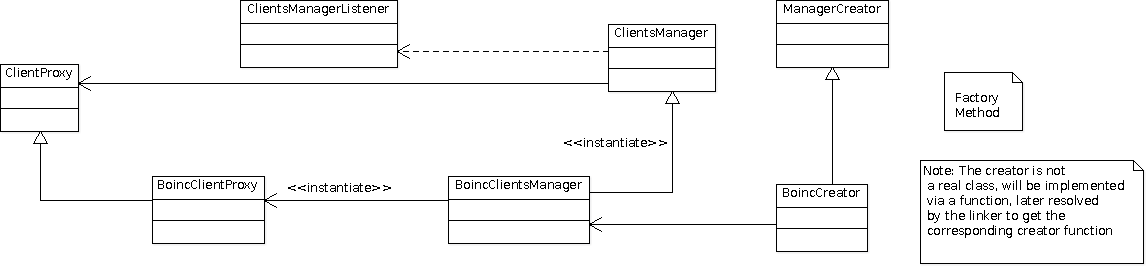
\includegraphics[scale=0.45]{images/Server_FuD-BOINC.png}
			\caption{Diseño de la capa de distribución del lado servidor}
			\label{fig:server-L1}
			\end{center}
	\end{figure} 

	\begin{figure}[H]
		\begin{center}
  			\vspace{100pt}
  			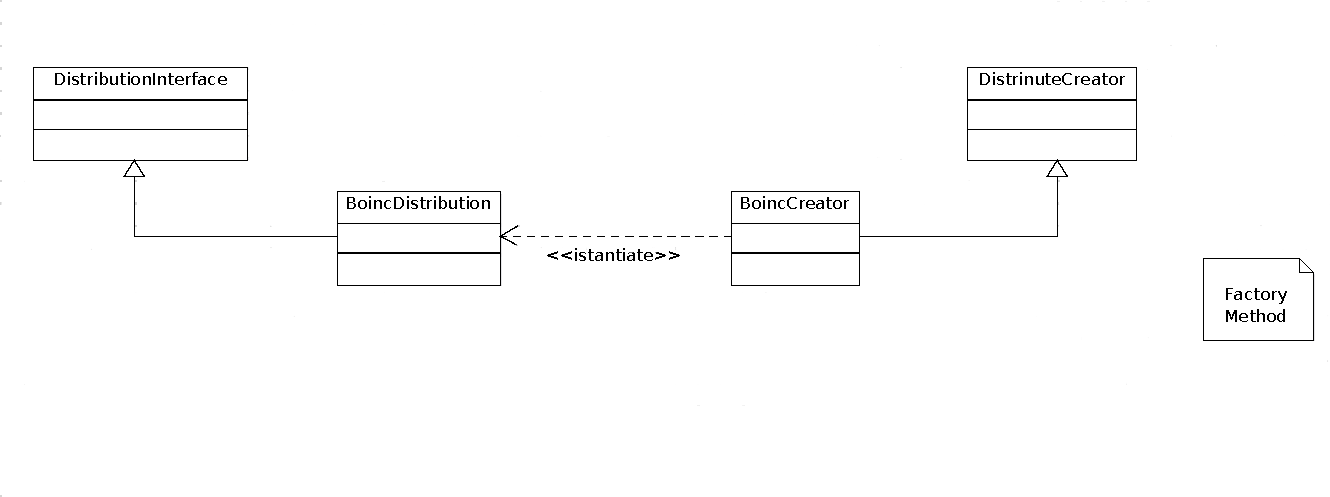
\includegraphics[scale=0.45]{images/Client_FuD-BOINC.png}
			\caption{Diseño de la capa de distribución del lado cliente}
			\label{fig:cliente-L1}
			\end{center}
	\end{figure} 
\end{landscape}

\subsection{Interacción entre FuD y BOINC}

Como se mencionó anteriormente, se hizo un trabajo de investigación muy importante que nos permitió determinar el tipo de interacción que debería existir entre FuD y BOINC. Por eso, fue necesario diferenciar correctamente la funcionalidad de cada uno de los módulos de ambos frameworks, y cómo ellos debían relacionarse.

En una primera instancia, se hizo un análisis abstracto que permitió dar un panorama general sobre cómo debían interactuar ambos frameworks. La figura \ref{fig:interaccion-fud-boinc-general} muestra dicha interacción en donde puede observarse que la capa inferior L1 de FuD-server es la encargada de comunicarse con el servidor BOINC el cual, a su vez, mantiene una comunicación con cada cliente por medio de BOINC Manager quien es el encargado de ejecutar la aplicación cliente de FuD pasándole el mensaje recibido. Lo mismo ocurre en el camino inverso desde el cliente al servidor, donde éste último recibe los resultados de la computación por parte del cliente. 

\begin{figure}[H]
	\begin{center}
  		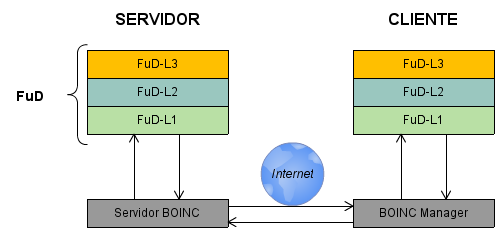
\includegraphics[scale=0.7]{images/interaccion-fud-boinc-general.png}
		\caption{Esquema general de comunicación entre FuD y BOINC}
		\label{fig:interaccion-fud-boinc-general}
	\end{center}
\end{figure}

El siguiente paso fue realizar un diagrama de secuencia que detallara aún más la interacción entre los módulos de FuD y BOINC necesarios para el cálculo de una \texttt{JobUnit}. La interacción exhibida en la figura \ref{fig:interaccion-fud-boinc} se repite por cada \texttt{JobUnit} que necesite ser computada.

\begin{landscape}
	\begin{figure}[H]
		\begin{center}
	  		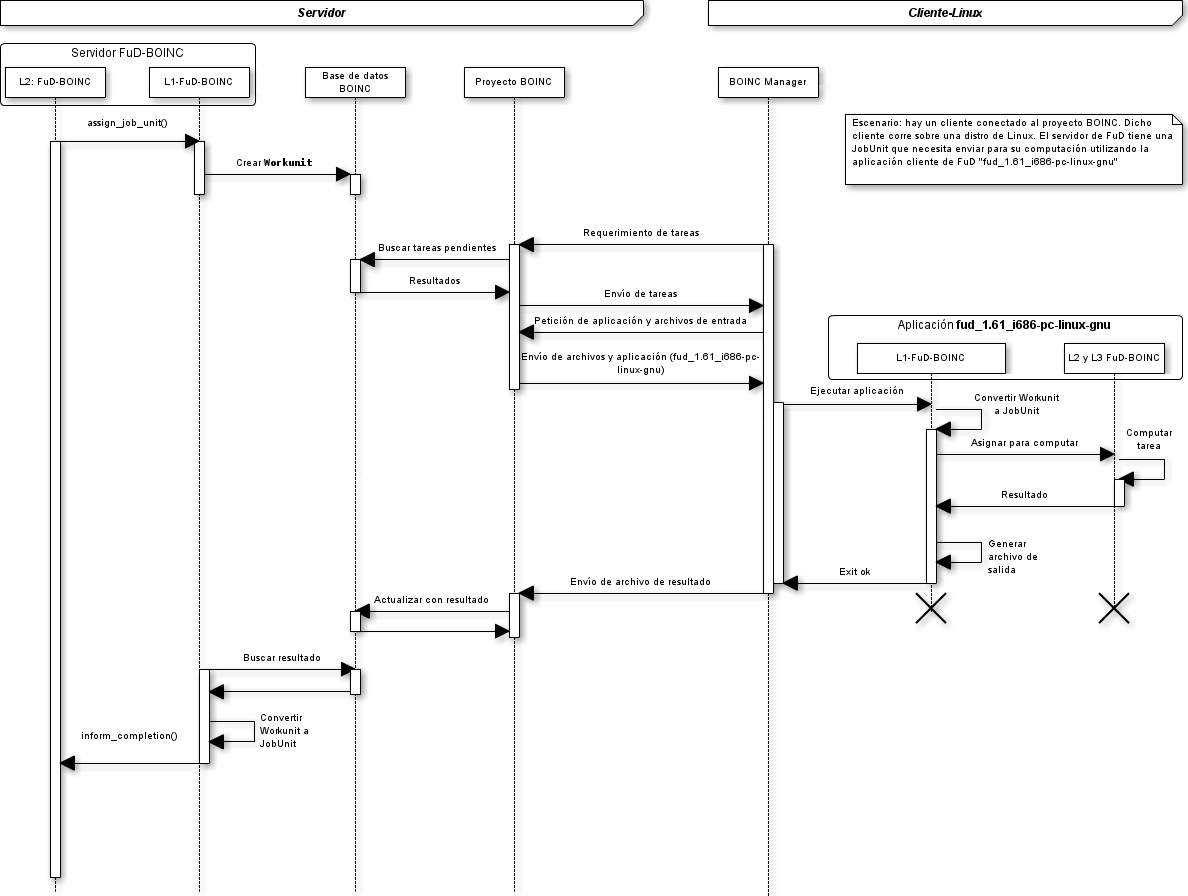
\includegraphics[scale=0.41]{images/interaccion-fud-boinc.png}
			\caption{Interacción necesaria entre FuD y la arquitectura BOINC para el cómputo de una \texttt{JobUnit}}
			\label{fig:interaccion-fud-boinc}
		\end{center}
	\end{figure}
\end{landscape}


\section{Diseño de bajo nivel}

Aquí se hace un refinamiento de las decisiones de diseño sobre aquellos componentes abstractos presentes en el diseño de alto nivel. También se analiza cómo estas clases están compuestas: los atributos de cada una, los métodos que declara y su interacción con el resto del sistema.

Para el desarrollo de FuD-BOINC, el mayor esfuerzo se debió enfocar en esta parte del diseño debido a que a partir de la vista estructural de la capa de distribución de FuD se tuvieron que especificar los nuevos módulos como así también sus principales variables y funciones. 

A continuación se muestran las clases que componen el diseño de FuD-BOINC:

\subsection{Servidor}

\subsubsection{BoincClientsManager}
\label{section:BoincClientsManager}
Es una clase que hereda directamente de la clase \texttt{ClientsManager} de FuD y está encargada del manejo de clientes del mismo. Si bien esta caractersística de múltiples clientes se hereda de FuD, la realidad es que FuD-BOINC solo debe administrar un único cliente conectado y disponible permanentemente. La existencia de un único cliente conectado permite que L2 asigne las \texttt{JobUnits} inmediatamente a L1 la cual las deberá reflejar acordemente en la base de datos del proyecto BOINC. Luego, es el framework de BOINC el encargado de realizar las conexiones con los clientes finales (voluntarios) para el envío dichas tareas.

Además, como el servidor del proyecto BOINC se encarga de reenviar aquellas tareas fallidas o no computadas, para esta implementación fue necesario deshabilitar el reenvío de \texttt{JobUnits} por parte de FuD ya que por defecto son reenviadas cuando las mismas no son informadas. 
Por lo tanto, al heredar de \texttt{ClientsManager} se debió proveer de esta funcionalidad, que en este caso fue introducida al realizar el rediseño de FuD descripto en la sección \ref{seccion:rediseno:fud}:

\begin{itemize}
\item \texttt{bool should\_resend\_job\_units()}: su función es determinar si la implementación de la capa L1 permite el reenvío de \texttt{JobUnits}. Este método es utilizado por el \texttt{JobManager}, perteneciente a la capa L2 de FuD, para determinar si debe volver a enviar aquellas \texttt{JobUnits} que aún no fueron reportadas por los nodos de procesamiento.
\end{itemize}

La figura \ref{fig:BoincClientsManager} muestra el diseño de la clase \texttt{BoincClientsManager}:

\begin{figure}[H]
	\begin{center}
  		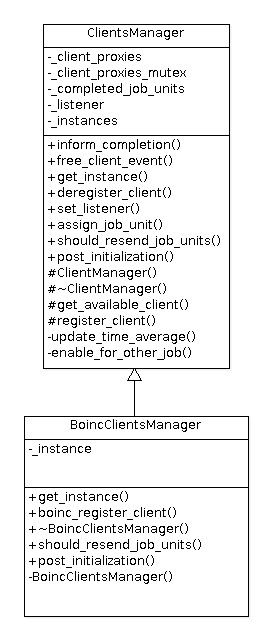
\includegraphics[scale=0.65]{images/BoincClientsManager.png}
		\caption{Clase BoincClientsManager}
		\label{fig:BoincClientsManager}
		\end{center}
\end{figure} 


\subsubsection{BoincClientProxy}

La clase \texttt{BoincClientProxy} hereda directamente de la clase \texttt{ClientProxy} de FuD y representa a un cliente conectado para la capa L1 de éste framework; en el caso de esta implementación, una instancia de \texttt{BoincClientProxy} representa una conexión con el servidor de BOINC, más precisamente con su base de datos.

Su función principal es la de crear y mantener una conexión directa con el servidor BOINC por medio de la cual notificará sobre las tareas a computar y se encargará de obtener los resultados recibidos de las computaciones realizadas por los voluntarios del proyecto. 

Como se dijo en el punto anterior, para representar la existencia de un único cliente conectado es importante que exista una única instancia de esta clase que será manejada por \texttt{BoincClientsManager}.

Es importante dejar en claro que el hecho de que FuD-BOINC considere disponible en todo momento al servidor de BOINC no implica que dicho servidor esté corriendo o detenido ya que la comunicación de la capa L1 se realiza directamente con la base de datos del proyecto. De esta manera, el servidor de FuD-BOINC podría correr y generar tareas en la base de datos del proyecto las cuales serán enviadas a los clientes una vez que el servidor sea iniciado.

La estructura de \texttt{BoincClientProxy} puede verse en la figura \ref{fig:BoincClientProxy}:

La funcionalidad heredada que debe ser provista a FuD mediante esta clase es la siguiente:

\begin{itemize}
\item \texttt{void process(const JobUnit\& job\_unit)}: su función es enviar la \texttt{JobUnit} a un cliente para su procesamiento. La implementación de este método depende del tipo de \texttt{ClientsManager} utilizado, en este caso \texttt{BoincClientsManager}.
\end{itemize}

\begin{figure}[H]
	\begin{center}
  		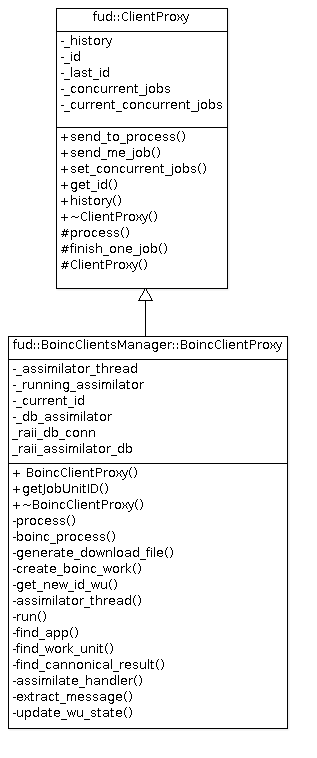
\includegraphics[scale=0.65]{images/BoincClientProxy.png}
		\caption{Clase BoincClientProxy}
		\label{fig:BoincClientProxy}
	\end{center}
\end{figure} 


\subsection{Cliente}

\subsubsection{BoincDistribution}
\label{seccion:diseno:BoincDistribution}
Esta clase hereda de la clase abstracta \texttt{DistributionClient} de FuD y provee la funcionalidad necesaria para la comunicación con el servidor. En el caso de este proyecto, la comunicación directa entre cliente y servidor de FuD no existe ya que BOINC es el encargado de llevar a cabo dicha tarea. Por el contrario, esta clase es la encargada de interpretar la \texttt{workunit} brindada por BOINC Manager \ref{boinc:manager} cuando éste ejecuta la aplicación cliente de FuD. Luego, al finalizar la computación de la tarea, se ocupa de escribir los resultados en un archivo de salida para que BOINC Manager lo informe al servidor.

Básicamente, su función es de traducir la \texttt{workunit} de BOINC a \texttt{JobUnit}, informar de la \texttt{JobUnit} a su capa superior, y luego realizar el proceso inverso.

La figura \ref{fig:BoincDistribution} muestra el diseño de esta clase:

\begin{figure}[H]
	\begin{center}
  		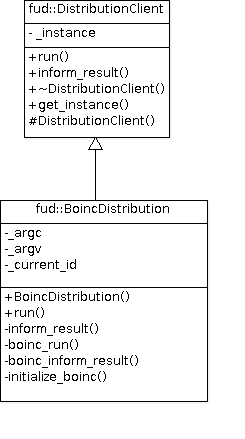
\includegraphics[scale=0.65]{images/BoincDistribution.png}
		\caption{Clase BoincDistribution}
		\label{fig:BoincDistribution}
	\end{center}
\end{figure}

Las funcionalidades más importantes de \texttt{BoincDistribution} deben ser provistas por los siguientes métodos:

\begin{itemize}
\item \texttt{void run()}: es el método encargado de iniciar la comunicación con el server. En este caso, se encarga de iniciar el proceso de traducción de la \texttt{workunit} a \texttt{JobUnit}.
\item \texttt{void inform\_result(bool result)}: su función es la de informar al servidor el resultado de la computación. En este caso, se encarga de escribir el resultado en un archivo binario.
\item \texttt{fud::create\_distribution\_client(int argc, char** argv)}: método encargado de la creación de una instancia de \texttt{DistributionClient}. En este caso, se crea una instancia de \texttt{BoincDistribution}.
\end{itemize}

		\chapter{Implementación}
\label{chapter:implementacion}

Este capítulo describe en detalle cómo algunas de las soluciones surgidas en el diseño fueron codificadas para resolver los requerimientos del problema original.

A continuación se explican algunas de las funcionalidades más relevantes denotadas en la etapa de diseño.


\section{Servidor FuD-BOINC}
La implementación del servidor FuD-BOINC se llevó a cabo sobre el sistema operativo Linux por dos motivos: por un lado, porque FuD y sus dependencias solo soportaban este sistema, y por el otro, porque el servidor de BOINC debe correr bajo este sistema operativo\footnote{\url{http://www.spy-hill.com/help/boinc/Create_Project.html\#server}}. Asimismo, en todo momento se trató de escribir código portable utilizando las librerías estándares.

	\subsection{BoincClientsManager}
Para proporcionar la funcionalidad de manejar un único cliente, con el inicio del sistema se hace una sola registración de un \texttt{BoincClientProxy} el cual perdurará durante toda la ejecución del servidor. De ésto se encarga el método \texttt{boinc\_register\_client()} el cual es invocado por el método \texttt{post\_initialization()} dentro del constructor \texttt{JobManager} de la capa L2. El último método mencionado forma parte de la reimplementación de FuD detallada en la sección \ref{seccion:jobmanager:post:init} de este proyecto. 

A continuación se muestra el código de la función \texttt{boinc\_register\_client()}:

\newpage

\begin{lstlisting}[frame=shadowbox, language=c++, numbers=left, xleftmargin=8mm, framexleftmargin=20pt, basicstyle=\footnotesize, numberstyle=\footnotesize, captionpos=b, caption={Método \texttt{boinc\_register\_client()} de la clase \texttt{BoincClientsManager}}, label=listing:BoincClientsManager:register:client, backgroundcolor=\color{gris}, firstnumber=66, keywordstyle=\color{Blue}]
void BoincClientsManager::boinc_register_client()
{
    // Init the client_proxy.
    boinc_log_debug(std::string(``Registering BOINC with FuD.''));
    BoincClientProxy * client = new BoincClientProxy();
    client->set_concurrent_jobs(UNLIMITED_JOBS);
    // Register the unique client proxy.
    register_client(client);
}
\end{lstlisting}

Por otro lado, bastó con que el método \texttt{should\_resend\_job\_units()} retorne \texttt{false} para indicar que FuD no reenvíe las \texttt{JobUnits}; tarea llevada a cabo por BOINC.
	
	\subsection{BoincClientProxy}
Si bien la creación de objetos \texttt{BoincClientProxy} es controlada por \texttt{BoincClientsManager}, se optó por utilizar el patrón de diseño Singleton para \linebreak restringir la creación de objetos de esta clase con el fin de evitar que se le dé un uso incorrecto en futuras implementaciones.

Esta es la clase más importante de la capa de distribución del lado servidor ya que es quien toma contacto con el proyecto BOINC mediante una conexión directa a su base de datos. Por esta razón, el constructor es el encargado de leer el archivo de configuración del proyecto BOINC (ver sección \ref{seccion:boinc:config:xml}) y de iniciar la conexión con la base de datos.

A continuación se muestra la implementación del constructor de la clase \texttt{BoincClientProxy}:

\begin{lstlisting}[frame=shadowbox, language=C++, numbers=left, xleftmargin=8mm, framexleftmargin=22pt, basicstyle=\scriptsize, numberstyle=\footnotesize, breaklines=true, breakatwhitespace=false, captionpos=b, caption={Constructor \texttt{BoincClientProxy}}, label=listing:BoincClientProxy, backgroundcolor=\color{gris}, firstnumber=83, keywordstyle=\color{Blue}]
BoincClientsManager::BoincClientProxy::BoincClientProxy() :
    ClientProxy(),
    _running_assimilator(true),
    raii_assimilator_db(db_assimilator),
    db_conn(boinc_db)
{
    set_log_level(LOG_HIGH);
    boinc_log_debug(std::string(``Parsing the BOINC config file.''));
    
    // Read the BOINC config file.
    int retval = config.parse_file();
    if (retval != RETVAL_OK)
    {
        std::string message =  ``Can`t parse BOINC config.xml file, '';
        message += boincerror(retval);
        throw (BoincFileException(message));
    }

    // Open the BOINC database.
    boinc_log_debug(std::string(``Connecting with the BOINC database.''));
    retval = boinc_db.open(config.db_name, config.db_host, config.db_user, config.db_passwd);
    if (retval != RETVAL_OK)
    {
        std::string message = ``Can`t open DB, '';
        message += boincerror(retval);
        throw (BoincDataBaseException(message));
    }

    //Creates assimilator thread to handle client response.
    _assimilator_thread = boost::thread( boost::bind( &BoincClientProxy::assimilator_thread, this ) );
}
\end{lstlisting}

La línea número 112 es la encargada de lanzar un nuevo hilo de ejecución el cual tiene como función notificar a la capa L2 los resultados recibidos por parte de los nodos de procesamiento. La sección \ref{seccion:asimilador} explica con más detalles la responsabilidad de este thread.

Otra de las funciones de esta clase es la de implementar el método \texttt{process()} provisto por FuD el cual es el encargado de enviar la \texttt{JobUnit} a un cliente. En este caso, la implementación de este método se encarga de serializar la \texttt{JobUnit} dentro de un archivo binario el cual va a ser utilizado para crear la \texttt{workunit} de BOINC. Toda esta funcionalidad a su vez se encuentra encapsulada dentro del método \texttt{boinc\_process()} el cual se describe a continuación:

\begin{lstlisting}[frame=shadowbox, language=C++, numbers=left, xleftmargin=8mm, framexleftmargin=22pt, basicstyle=\scriptsize, numberstyle=\footnotesize, breaklines=true, breakatwhitespace=false, captionpos=b, caption={Método \texttt{boinc\_process()} de \texttt{BoincClientProxy}}, label=listing:BoincClientProxy:boinc:process, backgroundcolor=\color{gris}, firstnumber=247, keywordstyle=\color{Blue}]
void BoincClientsManager::BoincClientProxy::boinc_process(const JobUnit& job_unit) 
                    throw(std::ofstream::failure, BoincAppException, BoincFileException, BoincWorkException )
{
    std::string name_input_file;
    generate_download_file(job_unit,name_input_file);

    // Read the wu_template.
    boinc_log_debug(std::string(``Reading the workunit template file''));
    char* wu_template;
    const int retval = read_file_malloc(config.project_path(WU_TEMPLATE.c_str()), wu_template);
    if (retval != RETVAL_OK)
    {
        std::string  description = ``Error in read_file_malloc, '';
        description += boincerror(retval);
        throw (BoincFileException(description));
    }

    create_boinc_work(name_input_file, wu_template);
}
\end{lstlisting}

El método invocado en la línea 251 es el encargado de crear el archivo binario con la información de la \texttt{JobUnit} dentro del directorio de descarga del proyecto para que los voluntarios lo descarguen cuando se le asigne la tarea asociada. En la línea 256 se lee la plantilla utilizada por BOINC en donde se especifica ciertas características que debe poseer la \texttt{workunit} a crear. Por último, en la línea 264 se lleva a cabo la creación de la \texttt{workunit} por medio de la invocación al método \texttt{create\_boinc\_work()}.

La implementación del método \texttt{create\_boinc\_work(std::string name\_input\_file, const char* wu\_template)} se puede simplificar en los siguientes pasos:

\begin{enumerate}
\item crear el nombre identificatorio de la \texttt{workunit},
\item obtener desde la base de datos la información de la aplicación asociada a esta tarea,
\item crear la \texttt{workunit} utilizando el nombre creado en el punto 1, la información de la aplicación obtenida en el punto 2, el archivo binario conteniendo la información de la \texttt{JobUnit} y la plantilla obtenida en la línea 256 del código  \ref{listing:BoincClientProxy:boinc:process} mencionada anteriormente. Para realizar este proceso se utiliza el método \texttt{create\_work()} provisto por BOINC\footnote{\url{http://boinc.berkeley.edu/trac/wiki/JobSubmission\#cpp-workgen}}.
\end{enumerate}

Por el contrario, la clase también se encarga de recuperar de la base de datos los resultados de las tareas enviadas. Para ello, se hizo la implementación de un asimilador de resultados.

	\subsubsection{Asimilador}
	\label{seccion:asimilador}
Una parte importante de la implementación de la clase \texttt{BoincClientProxy} consistió en poder integrar el comportamiento del demonio \textit{assimilator} (\ref{boinc:assimilator}) de BOINC como parte del comportamiento de esta clase al momento de manejar un resultado recibido desde el cliente. Debió realizarse esta integración ya que la manera en que BOINC propone la implementación de este demonio obliga a crear un nuevo ejecutable de manera independiente a la aplicación de FuD. Ésto evitaba respetar el modelo de FuD, en donde la misma aplicación debe encargarse de atrapar e interpretar los resultados de las tareas concluidas.

Por ello, el asimilador se implementa en un nuevo hilo de ejecución, utilizando \texttt{boost::thread}\footnote{\url{http://www.boost.org/}}, dentro del servidor FuD-BOINC encargándose de chequear la existencia de resultados no asimilados. Si la unidad de trabajo fue completada y validada satisfactoriamente por el demonio \textit{validator} (\ref{seccion:demonio:validator}), a partir de su resultado canónico, se lee el archivo de salida, se extrae su contenido (\texttt{JobUnit}) y se le informa a L2 sobre la terminación de dicha tarea. El método \texttt{run()} de la clase \texttt{BoincClientProxy} contiene la implementación de los pasos generales aquí descriptos:

\begin{lstlisting}[frame=shadowbox, language=C++, numbers=left, xleftmargin=8mm, framexleftmargin=22pt, basicstyle=\scriptsize, numberstyle=\footnotesize, breaklines=true, breakatwhitespace=false, captionpos=b, caption={Método \texttt{run()} de \texttt{BoincClientProxy}}, label=listing:BoincClientProxy:run, backgroundcolor=\color{gris}, firstnumber=285, keywordstyle=\color{Blue}]
void BoincClientsManager::BoincClientProxy::run() throw(BoincException)
{
    boinc_log_debug(std::string(``Starting the assimilator daemon.''));
    //  Open a new database's connection separated from the main process.
    const int retval = db_assimilator.open(config.db_name, config.db_host, config.db_user, config.db_passwd);
    if (retval != RETVAL_OK)
    {
        std::string message = ``The assimilator daemon can`t open DB: '';
        message += boincerror(retval);
        throw (BoincDataBaseException(message));
    }
    DB_APP app(&db_assimilator);
    DB_WORKUNIT wu(&db_assimilator);
    DB_RESULT canonical_result(&db_assimilator);
    std::stringstream buf();

    app = find_app(NAME_APP, db_assimilator);
    while(_running_assimilator)
    {
        if (find_work_unit(app, wu) == true)
        {   
            // Found a WU.
            if ( find_cannonical_result(wu,canonical_result) == true ) 
            {
                // Found a Canonical Result.
                assimilate_handler(wu,canonical_result);
                update_wu_state(wu, WuDone);                
            }
        }
        sleep(SLEEP_INTERVAL);
    }
}
\end{lstlisting}

En la línea número 304 se busca una workunit que no haya sido asimilada y en la línea 307 se examina si existe un resultado canónico para esa unidad de trabajo. Finalmente, si se encuentra un resultado canónico se lo asimila invocando al método \texttt{assimilate\_handler()} en la línea 310.

El método \texttt{assimilate\_handler()} es el encargado de leer y extraer la \texttt{JobUnit} encapsulada dentro del archivo binario asociado al resultado canónico. Una vez obtenido el mensaje de la \texttt{JobUnit} el mismo es informado a la capa L2 mediante la invocación al método \texttt{ClientsManager::get\_instance()->inform\_completion()} tal como lo especifica el diseño de FuD. La llamada secuencial de los métodos mostrados en el código \ref{listing:BoincClientProxy:assimilate:handler} representa la sección más importante del método \texttt{assimilate\_handler()}:

\begin{lstlisting}[frame=shadowbox, language=C++, numbers=left, xleftmargin=8mm, framexleftmargin=22pt, basicstyle=\scriptsize, numberstyle=\footnotesize, breaklines=true, breakatwhitespace=false, captionpos=b, caption={Líneas importantes del método \texttt{assimilate\_handler()}}, label=listing:BoincClientProxy:assimilate:handler, backgroundcolor=\color{gris}, texcl=true, firstnumber=424, keywordstyle=\color{Blue}]
std::string* msg = extract_message(output_file);
ClientsManager::get_instance()->inform_completion( getJobUnitID(), msg);
\end{lstlisting}
                

\section{Cliente FuD-BOINC}
Al igual que el servidor, la capa de distribución del cliente de FuD-BOINC fue desarrollada para sistemas operativos Linux. Sin embargo, como la plataforma cliente de BOINC está disponible para varios sistemas operativos y considerando que Windows es el más utilizado a nivel mundial, la implementación de la capa cliente de FuD-BOINC fue pensada para que pueda ser compilada tanto para Linux como para Windows, cumpliendo así con una de las metas del proyecto.

A continuación, bajo el título Linux, se explica la implementación llevada a cabo la cual es soportada por ambos sistemas operativos. Mientras que bajo el título Windows (\ref{seccion:cliente:windows}) se mencionan las tareas llevadas a cabo para lograr la compilación del cliente FuD-BOINC para este sistema operativo.

	\subsection{Linux}
	\subsubsection{BoincDistribution}
Como se detalló en la sección \ref{seccion:diseno:BoincDistribution}, la función principal de la clase \texttt{BoincDistribution} es la de interpretar el archivo de entrada pasado como argumento por el cliente de BOINC (\ref{boinc:manager}) y luego de generar un archivo con los resultados obtenidos.

El cliente de BOINC es el encargado de ejecutar la aplicación cliente de FuD y a su vez de pasarle por parámetro el archivo conteniendo la tarea a ejecutar. Por esta razón, como se explica en la sección \ref{rediseno:create:distr:client}, fue necesario modificar el método provisto por FuD para la creación de un cliente de distribución para que reciba los argumentos de la función \texttt{main} como parámetros.

Como se dijo anteriormente, el primer paso de \texttt{BoincDistribution} es el de leer el archivo binario que contiene encapsulada la \texttt{JobUnit} de FuD para luego informarla a su capa superior la cual se encargará de llevar a cabo dicha tarea. Las siguientes líneas de código son parte del método \texttt{boinc\_run()} de \texttt{BoincDistribution} y se encargan de realizar lo aquí detallado:\\

\begin{lstlisting}[frame=shadowbox, language=C++, numbers=left, xleftmargin=8mm, framexleftmargin=22pt, basicstyle=\scriptsize, numberstyle=\footnotesize, breaklines=true, breakatwhitespace=false, captionpos=b, caption={Parte del método \texttt{boinc\_run()} de la clase \texttt{BoincDistribution}}, label=listing:BoincDistribution:boinc:run, backgroundcolor=\color{gris}, firstnumber=139, keywordstyle=\color{Blue}]
std::ifstream ifs(file_name.c_str(), std::ios::binary);
// Enable file exceptions.
ifs.exceptions(std::ifstream::eofbit | std::ifstream::failbit | std::ifstream::badbit);

std::clog << ``FuD: extracting the input file for computation.'' << std::endl;
        
// Extract the content of the input file to deliver.
std::stringstream oss;
oss << ifs.rdbuf();
InputMessage input_msg (oss.str());

// Get the message and _current_id
std::string message;
input_msg >> _current_id >> message;

ProcessorsManager::get_instance()->deliver_message(message);
\end{lstlisting}

Las líneas 147 y 148 extraen el contenido del archivo binario dentro de un objeto \texttt{InputMessage} el cual es un alias del tipo \texttt{bistream} de mili\footnote{\url{http://code.google.com/p/mili/}}. En la línea 152 se obtiene el \textit{id} y el \textit{mensaje} de la \texttt{JobUnit} para luego en la línea 154 informar de la tarea a realizar.

Por el contrario, una vez que la computación es finalizada, L2 informa de ésto a L1 mediante el método \texttt{inform\_result()} para que se encargue de enviar los resultados al servidor. En ese momento es cuando se inicia la creación del archivo binario con los resultados de la computación. Este proceso se realiza dentro del método \texttt{boinc\_inform\_result()}. El código \ref{listing:BoincDistribution:boinc:inform:result} muestra las líneas más importantes:

\begin{lstlisting}[frame=shadowbox, language=C++, numbers=left, xleftmargin=8mm, framexleftmargin=22pt, basicstyle=\scriptsize, numberstyle=\footnotesize, breaklines=true, breakatwhitespace=false, captionpos=b, caption={Parte del método \texttt{boinc\_inform\_result()} de la clase BoincDistribution}, label=listing:BoincDistribution:boinc:inform:result, backgroundcolor=\color{gris}, firstnumber=74, keywordstyle=\color{Blue}]
std::string body = ProcessorsManager::get_instance()->get_return_message();

OutputMessage bos;
bos << _current_id << body;

// File to upload to server.
std::ofstream out;

//enable the exceptions
out.exceptions ( std::ofstream::failbit | std::ofstream::badbit );
out.open(file_name.c_str(), std::ios::binary);

// Get the message with result of computation to send back to server.
out << bos.str();
\end{lstlisting}

Aquí, en la línea 76 se crea un objeto \texttt{OutputMessage} con el \textit{id} y el \textit{mensaje} conteniendo el resultado de la tarea computada. En la línea 87 se escribe el \texttt{OutputMessage} dentro del archivo binario.

Es importante mencionar que el contenido que se almacena dentro de los archivos binarios, enviados desde el servidor y desde el cliente, son de tipo \texttt{OutputMessage} el cual FuD lo define como un alias de \texttt{bostream} de mili. Por ello, en la extracción del contenido de dicho archivo se utiliza un \texttt{InputMessage} de FuD quien lo define como un alias de \texttt{bistream} de mili.

	\subsection{Windows}
	\label{seccion:cliente:windows}
Como se mencionó al comienzo de esta sección, fue necesario compilar el cliente de FuD-BOINC para sistemas operativos Windows ya que son los más utilizados actualmente. Desde el principio del desarrollo de este proyecto se conoció este requerimiento y por eso fue que se trató de escribir código portable en todo momento para que al llegar a esta etapa no surgieran grandes modificaciones. 

El IDE utilizado para esta tarea fue Microsoft Visual C++ 2005 Express Edition\footnote{\url{http://www.microsoft.com/visualstudio/en-us/products/2010-editions/express/}} al cual se desconocía por completo, motivo por el cual los tiempos se extendieron más de lo previsto.

Los cambios realizados en este proceso de compilación fueron diversos. A continuación se enumeran los pasos más generales que nos permitieron lograr este objetivo:

\begin{enumerate}
\item Compilar las librerías BOINC.
\item Generar y configurar un proyecto solución de Visual Studio para la compilación.
\item Resolver dependencias con las librerías: boost\footnote{\url{http://www.boost.org/}}, pthread\footnote{\url{http://sourceware.org/pthreads-win32/}}, mili\footnote{\url{http://code.google.com/p/mili/}} y MySQL\footnote{\url{http://dev.mysql.com/downloads/connector/cpp/}}.
\item Modificar el tipo de \texttt{include} realizado por algunos de los archivos del cliente de FuD al detectar la macro \texttt{\_WIN32}.
\item Por último, compilar el cliente de FuD.
\end{enumerate}

	
\section{Headers utilizados por servidor y cliente}
Bajo el directorio \texttt{common} del middleware se alojan tres archivos que son utilizados tanto por el servidor como el cliente de FuD-BOINC. Estos archivos proveen de constantes y excepciones utilizadas por esta capa:
	\begin{itemize}
		\item \texttt{boinc\_common.h}: incluye a \texttt{boinc\_constants.h} y define tipos enumerados que son utilizados por el servidor y el cliente.
		\item \texttt{boinc\_constants.h}: define constantes útiles que permiten escribir código legible a la hora de interpretar los valores utilizados por métodos específicos de BOINC.
		\item \texttt{boinc\_exception.h}: este módulo define excepciones específicas que puede generar una aplicación FuD-BOINC ante la presencia de un fallo. Todas estas excepciones se definieron a partir de \texttt{generic\_exceptions} de mili.
\end{itemize}


\section{Archivos de configuración \texttt{CMakeLists.txt}}
La adaptación al diseño de FuD incluyó además ajustarse al proceso de compilación de la librería. FuD utiliza CMake (\ref{tool:cmake}) para la generación de Makefiles que permiten llevar a cabo la compilación, por lo que cada directorio del proyecto cuenta con un archivo \texttt{CMakeLists.txt} compuesto de varias sentencias. 

Por consiguiente, lo que se hizo al respecto fue seguir la configuración de generación original de FuD de manera que el usuario pueda especificar por línea de comandos el tipo de compilación que desea realizar y con qué capa de distribución desea que FuD trabaje. Para ello, fue necesario hacer modificaciones en los \texttt{CMakeLists.txt} originales de FuD y a su vez agregar un archivo \texttt{CMakeLists.txt} dentro de cada directorio de la capa de distribución. Aquí, el directorio mayor en la jerarquía es quien contiene el archivo de configuración encargado de resolver todas las dependencias de aquellas librerías requeridas por el framework BOINC.

Si algunas de las dependencias requeridas no pueden ser resuelta, CMake informará de dicho error y cancelará el proceso de generación.

\section{mili::RAII}
A medida que se avanzaba con la implementación de este proyecto, desde la fundación, se sugirió utilizar RAII\footnote{\url{http://en.wikipedia.org/wiki/Resource_Acquisition_Is_Initialization/}} para liberar recursos de manera segura ante la presencia de imprevistos. Además, para que la solución pueda ser reutilizada en otros proyectos de FuDePAN, se decidió entonces desarrollar una solución genérica e incluirla como parte de la librería mili\footnote{\url{http://code.google.com/p/mili/}}. 

Finalmente, se utilizó la librería \texttt{mili::RAII} para la liberación segura de recursos.

\subsection{Problema}
El problema que dio origen a esta implementación fue que los objetos de tipo \texttt{DB\_CONN} provistos por la API de BOINC para la conexión con la base de datos no cuentan con un destructor que se encargue de cerrar la conexión y liberar la memoria utilizada por la misma. Por este motivo, debíamos invocar manualmente al operador \texttt{DB\_CONN::close()}.

\subsection{Solución}
El código \ref{listing:mili:raii} muestra la clase genérica implementada en mili\footnote{\url{http://code.google.com/p/mili/source/browse/trunk/mili/raii.h}} que soluciona el problema planteado:

\begin{lstlisting}[frame=shadowbox, language=C++, numbers=left, xleftmargin=8mm, framexleftmargin=22pt, basicstyle=\scriptsize, numberstyle=\footnotesize, breaklines=true, breakatwhitespace=false, captionpos=b, caption={Implementación RAII de la librería mili}, label=listing:mili:raii, backgroundcolor=\color{gris}, firstnumber=74, keywordstyle=\color{Blue}]
#ifndef RAII_H
#define RAII_H

NAMESPACE_BEGIN

template <class T, void (T::*M)(void)>
class RAII
{

public:
    RAII(T& inst) : _var(inst) {}
    ~RAII()
    {
        (_var.*M)();
    }

private:
    T& _var;
};

NAMESPACE_END

#endif
\end{lstlisting}


\section{Rediseños de FuD}
\label{seccion:rediseno:fud}

Durante el desarrollo de este proyecto se debieron efectuar diversos cambios en el diseño e implementación original de FuD para poder integrar esta capa de distribución como capa opcional a la hora de utilizar la librería. Todos los cambios efectuados fueron pensados para mantener la compatibilidad con el resto de las capas de distribución desarrolladas y conservando el comportamiento e interfaz provisto para la implementación de una nueva capa.

A continuación se detallan los puntos que fueron rediseñados y que agregan nuevas características a FuD.

\subsection{Redeclaración del método \texttt{create\_distribution\_client()}}
\label{rediseno:create:distr:client}

\subsubsection{Problema}
El método original provisto por FuD para la creación de un cliente de distribución en la función \texttt{main} tenía el siguiente prototipo:

\texttt{DistributionClient* create\_distribution\_client(std::string address, Port port)}\\

Ésto obligaba a la capa de distribución a utilizar un \texttt{address} y un \texttt{port} en su creación. Para el caso de este proyecto esos valores no eran necesarios mientras que si eran importantes los valores recibidos como parámetros en la ejecución de la aplicación cliente por parte del cliente BOINC. Cuando el cliente BOINC ejecuta la aplicación cliente de FuD debe pasarle como argumento el nombre del archivo que contiene la tarea a computar, es decir \texttt{argv}. Por lo tanto, este prototipo resulta ser totalmente incompatible. 

\subsubsection{Solución}
La solución a este problema fue simplemente cambiar su prototipo para que sus parámetros coincidan con los argumentos de la función \texttt{main} que debe implementar la capa L3 de FuD. De esta manera, las implementaciones de la capa de distribución pueden recibir cualquier valor en el momento en que una aplicación es iniciada. Para el caso de la capa de distribución implementada con ASIO\footnote{\url{http://www.boost.org/doc/libs/1_48_0/doc/html/boost_asio.html}}, la dirección IP y el puerto pueden ser pasadas sin inconvenientes mediante línea de comandos o bien configurando el valor de \texttt{argv} con los valores correspondientes manteniendo así la compatibilidad.

El nuevo prototipo del método es el siguiente:\\

\texttt{DistributionClient* create\_distribution\_client(int argc, char** argv)}\\


\subsection{\texttt{JobManager} post initialization}
\label{seccion:jobmanager:post:init}

	\subsubsection{Problema}
FuD es orientado a eventos generados por clientes. Cuando un cliente se conecta al servidor, como primera instancia, debe registrase. Esta registración genera un nuevo evento de \textit{cliente libre} que provoca que el scheduler le asigne una tarea, siempre y cuando haya una disponible. Ahora bien, como los clientes de FuD-BOINC no se conectan con el servidor sino que solo se encargan de ejecutar la tarea recibida por parámetro, el evento mencionado nunca era generado por lo que el servidor nunca iniciaba su scheduler. Por consiguiente, el servidor nunca generaba tareas.
	
	\subsubsection{Solución}
La solución a este problema fue realizar la registración del cliente que representa al servidor BOINC inmediatamente después de la creación del \texttt{ClientsManager}. Como este objeto es creado en el constructor de la clase \texttt{JobManager} se decidió entonces agregar un nuevo método virtual a la clase \texttt{ClientsManager} llamado \texttt{post\_initialization()} en donde su implementación por defecto sea vacía para mantener así compatibilidad con las capas de distribución disponibles para FuD. Luego, al final del código del constructor del \texttt{JobManager} realizar la invocación a este método.

Para el caso de esta capa de distribución, el método es reimplementado por su clase derivada \texttt{BoincClientsManager} codificando allí la registración del único cliente con el cual va a contar el servidor FuD-BOINC.

A continuación, la figura \ref{fig:ClientsManager:orig} muestra el diseño original de la clase \texttt{ClientsManager} mientras que la figura \ref{fig:ClientsManager:actual} presenta el diseño actual de la clase. Tener en cuenta que aquí sólo se hace mención al método \texttt{post\_initialization()} por lo que el resto de las operaciones agregadas no deberían ser consideradas en este punto.

\begin{figure}[H]
	\hfill
	\begin{minipage}[t]{.4\textwidth}
		\begin{center}
	  		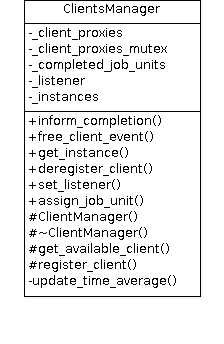
\includegraphics[scale=0.65]{images/ClientsManager-orig.png}
			\caption{Diseño original de la clase \texttt{ClientsManager}}
			\label{fig:ClientsManager:orig}
		\end{center}
	\end{minipage}
	\hfill
	\begin{minipage}[t]{.4\textwidth}
		\begin{center}
	  		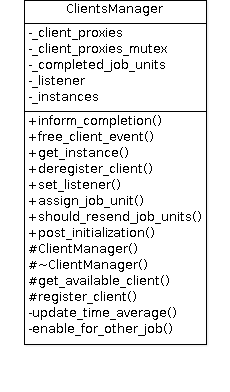
\includegraphics[scale=0.65]{images/ClientsManager-actual.png}
			\caption{Diseño actual de la clase \texttt{ClientsManager}}
			\label{fig:ClientsManager:actual}
		\end{center}
	\end{minipage}
	
\end{figure}

La declaración del método dentro de la clase \texttt{ClientsManager} es la siguiente:\\

\texttt{virtual void post\_initialization() \{\};}\\

Al constructor de la clase \texttt{JobManager} (código \ref{listing:fud:jobmanager}) se le agregó la línea 76 en donde puede observarse la invocación al método mencionado.

\begin{lstlisting}[frame=shadowbox, language=C++, numbers=left, xleftmargin=8mm, framexleftmargin=22pt, basicstyle=\scriptsize, numberstyle=\footnotesize, breaklines=true, breakatwhitespace=false, captionpos=b, caption={Código del constructor de la clase \texttt{JobManager}}, label=listing:fud:jobmanager, backgroundcolor=\color{gris}, firstnumber=56, keywordstyle=\color{Blue}]
JobManager::JobManager() :
    _clients_manager(create_clients_manager()),
    _producingJobs(),
    _waitingJobs(),
    _jobQueue(),
    _pendingList(),
    _ids_to_job_map(),
    _current_job_unit_size(10), //yes, hardcoded to begin with.
    _status(kStopped),
    _mutex(),
    _event_queue()
{
    timeval tm;
    gettimeofday(&tm, NULL);

    openlog(``FUD'', NULL, LOG_LOCAL1);
    syslog(LOG_NOTICE, ``Started FuD.'');

    _clients_manager->set_listener(this);

    _clients_manager->post_initialization();
}
\end{lstlisting}

Por último, la reimplementación de este método en \texttt{BoincClientsManager} realiza la registración del cliente invocando a \texttt{boinc\_register\_client()}:

\begin{lstlisting}[frame=shadowbox, language=C++, numbers=left, xleftmargin=8mm, framexleftmargin=22pt, basicstyle=\scriptsize, numberstyle=\footnotesize, breaklines=true, breakatwhitespace=false, captionpos=b, caption={Código del método \texttt{boinc\_register\_client()} de la clase \texttt{BoincClientsManager}}, label=listing:BoincClientsManager:boinc:register:client, backgroundcolor=\color{gris}, firstnumber=66, keywordstyle=\color{Blue}]
void BoincClientsManager::boinc_register_client()
{
    // Init the client_proxy.
    boinc_log_debug(std::string(``Registering BOINC with FuD.''));
    BoincClientProxy * client = new BoincClientProxy();
    client->set_concurrent_jobs(UNLIMITED_JOBS);
    // Register the unique client proxy.
    register_client(client);
}
\end{lstlisting}


\subsection{Reenvío de \texttt{JobUnits} configurable}
\label{seccion:reenvio:jobunits}

	\subsubsection{Problema}
Luego de resolver la sección anterior (\ref{seccion:jobmanager:post:init}) se encontró el siguiente problema: cada \texttt{JobUnit} que necesitaba ser computada era enviada dos veces por FuD por lo que en cada envío la capa de distribución creaba un \texttt{workunit} distinta. El reenvío de tareas por parte de FuD es normal ya que cuando no hay más trabajos para ser enviados, el framework comienza a reenviar aquellas tareas que aún no han sido reportadas por clientes.

Ésto no era necesario ya que el proyecto BOINC se encarga automáticamente de enviar aquellas tareas que aún no han sido reportadas. Además, esta característica particular de FuD agregaba \texttt{workunits} duplicadas en la base de datos del servidor BOINC innecesariamente ya que BOINC, dependiendo de la configuración del proyecto, replica cada \texttt{workunit}.

	\subsubsection{Solución}
La solución planteada fue que cada manejador de clientes deba especificar si el scheduler de FuD debe reenviar o no las tareas que no hayan sido informadas. Ésto permite que cada capa de distribución pueda decidir si deja que el scheduler reenvíe las tareas, si es ella quien brindará el servicio o bien si la característica queda deshabilitada en su totalidad. Para el caso de BOINC esta característica debe ser deshabilitada por el motivo mencionado anteriormente.

Por consiguiente, el método público agregado dentro de la clase \texttt{ClientsManager} en este caso fue el siguiente:\\

\texttt{virtual bool should\_resend\_job\_units() = 0;}\\

Las figuras \ref{fig:ClientsManager:orig} y \ref{fig:ClientsManager:actual} muestran el diseño original y actual de la clase \texttt{ClientsManager}. En las figuras considerar únicamente el método should\_resend\_job\_units() ya que el resto de las operaciones agregadas no forman parte de esta solución.

Una vez hecho ésto se debió reimplementar el método \texttt{handle\_free\_client\_event()} de la clase \texttt{JobManager} de la capa L2 de FuD para que consulte si se deben reenviar los trabajos. 

El código \ref{listing:jobmanager:handle:free:client} muestra una parte de la implementación de dicho modo. Las líneas 172, 173 y 185 fueron las agregadas para resolver el problema. 
\newpage
\begin{lstlisting}[frame=shadowbox, language=C++, numbers=left, xleftmargin=8mm, framexleftmargin=22pt, basicstyle=\scriptsize, numberstyle=\footnotesize, breaklines=true, breakatwhitespace=false, captionpos=b, caption={Parte del código del método \texttt{handle\_free\_client\_event()} de la clase \texttt{JobManager}}, label=listing:jobmanager:handle:free:client, backgroundcolor=\color{gris}, firstnumber=170, tabsize=4, keywordstyle=\color{Blue}]
if (_jobQueue.empty())
{
	if (_clients_manager->should_resend_job_units()) 
	{
		if (! _pendingList.empty())
		{
			if (_clients_manager->assign_job_unit(*_pendingList.front()))
			{
				//send this one to the back, act as Round Robin
				_pendingList.push_back(_pendingList.front());
				_pendingList.pop_front();
			}
			else
			syslog(LOG_NOTICE, ``Error sending JobUnit %u from Pending List to a client.'', _pendingList.front()->get_id());
		}
	}
}
\end{lstlisting}


\subsection{Múltiples \texttt{JobUnits} a clientes}
\label{seccion:multiples:jobunits:clientes}

	\subsubsection{Problema}
Si bien la primera vez que se ejecutó la aplicación Parallel-Clusterer\footnote{\url{http://code.google.com/p/parallel-clusterer/}} sobre FuD-BOINC en Linux finalizó correctamente, se advirtió que su desempeño no era el esperado debido a que solo se enviaban dos \texttt{JobUnits} a la vez lo que provocaba que su ejecución fuera excesivamente lenta.

Luego de investigar en detalle cómo era el proceso de asignación de tareas de FuD, se observó que el problema se encontraba relacionado directamente con los eventos administrados por la capa de manejo de trabajos (L2) ya que al iniciar la aplicación se generaban solo dos eventos de este tipo provocados, primero, por la presencia de un \texttt{DistributableJob} listo para producir, y segundo por la registración del único cliente al servidor.

La creación de dichos eventos se generan invocando al método \texttt{free\_client\_event()} de la clase \texttt{JobManager}. Luego, el scheduler de FuD, por cada uno de estos eventos intenta asignar una nueva tarea a aquellos clientes que no se encuentren ocupados. Como el único cliente de esta capa siempre se encuentra disponible, ambas tareas eran asignadas inmediatamente pero se debía esperar a que alguna de ellas finalizara ya que en ese momento es cuando se vuelve a generar un nuevo evento de \textit{cliente libre}. 

Es por ello, que el envío de trabajos no funcionaba como se esperaba debido a que el diseño original de FuD solo permitía que el cliente pueda procesar a lo sumo de a una \texttt{JobUnit} por vez.

	\subsubsection{Solución}
La solución que permitió eliminar este problema derivó en un rediseño para permitir que los clientes puedan ejecutar múltiples tareas a la vez. Para ello se debió dar soporte a la capa de distribución.

La idea general que resuelve lo planteado consiste en:

\begin{enumerate}
\item permitir que un cliente, en el momento de su creación, pueda configurar la \textit{cantidad máxima} de tareas que puede ejecutar al mismo tiempo;
\item llevar un registro de la \textit{cantidad de tareas} que un cliente se encuentra computando en un determinado momento. Con cada asignación de tarea este valor será incrementado y con cada informe de resultado será decrementado;
\item determinar si un cliente se encuentra disponible para computar otra tarea basándose de los valores configurados en los dos puntos anteriores;
\item si el cliente no llegó al límite de su capacidad configurada en el punto 1, generar un nuevo evento de \textit{cliente libre}.
\end{enumerate}

A continuación se detalla cada cambio realizado en las clases \texttt{ClientProxy} y \texttt{ClientsManager} en el orden mencionado:

\texttt{\\ClientProxy}:\\

Del diseño original de la clase \texttt{ClientProxy} (\ref{fig:ClientProxy:orig}) se \textit{\textbf{modificaron}} las siguientes operaciones:
\begin{itemize}
\item \texttt{process()}: se cambió su visibilidad pública a protegida manteniendo su prototipo original:\\
\texttt{virtual void process(const JobUnit\& job\_unit) = 0;}

\item \texttt{i\_am\_free()}: el método fue eliminado y reemplazado por \texttt{finish\_one\_job()}.

\item \texttt{busy()}: el método fue eliminado y reemplazado por \texttt{send\_me\_job()}.
\end{itemize}

Al diseño original de la clase \texttt{ClientProxy} (\ref{fig:ClientProxy:orig}) se \textit{\textbf{agregaron}} los siguientes atributos y métodos:

\begin{itemize}
\item \texttt{finish\_one\_job()}: encargado de generar un evento de \textit{cliente libre} y de decrementar a \texttt{\_current\_concurrent\_jobs}. Este método es invocado cuando una tarea es terminada. Su prototipo es:\\
\texttt{void finish\_one\_job();}

\item \texttt{send\_me\_job()}: comprueba si el cliente puede procesar otra tarea en simultáneo o bien si se encuentra ocupado. Su prototipo es:\\
\texttt{bool send\_me\_job() const}

\item \texttt{send\_to\_process()}: se encarga de enviar la \texttt{JobUnit} invocando al método \texttt{process()} y de incrementar a \texttt{\_current\_concurrent\_jobs}. Su prototipo es:\\
\texttt{void send\_to\_process(const JobUnit\& job\_unit);}

\item \texttt{\_concurrent\_jobs}: atributo de la clase que indica el total de tareas en simultáneo que puede computar el cliente. El valor 0 indica que el cliente puede procesar un número ilimitado de tareas en simultáneo (diseñado para BOINC). La constante \texttt{UNLIMITED\_JOBS} representa a dicho valor.

\item \texttt{\_current\_concurrent\_jobs}: atributo de la clase que indica la cantidad de tareas en simultáneo que está computando el cliente en un momento determinado.
\end{itemize}

\begin{figure}[H]
	\hfill
	\begin{minipage}[t]{.4\textwidth}
		\begin{center}
	  		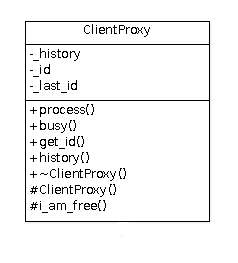
\includegraphics[scale=0.65]{images/ClientProxy-orig.png}
			\caption{Diseño original de la clase \texttt{ClientProxy}}
			\label{fig:ClientProxy:orig}
		\end{center}
	\end{minipage}
	\hfill
	\begin{minipage}[t]{.4\textwidth}
		\begin{center}
	  		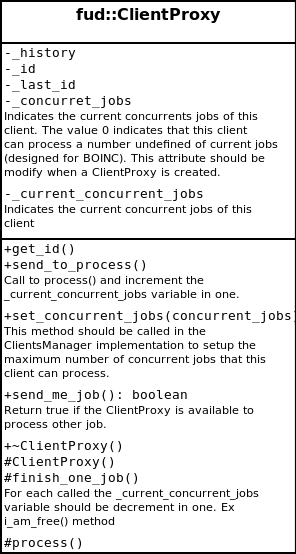
\includegraphics[scale=0.55]{redesing-multiplesJobs-on-client/ClientProxy.png}
			\caption{Diseño actual de la clase \texttt{ClientProxy}}
			\label{fig:ClientProxy:actual}
		\end{center}
	\end{minipage}
\end{figure}

\texttt{\\ClientsManager}:\\

Del diseño original de la clase \texttt{ClientsManager} (\ref{fig:ClientsManager:orig}) se \textbf{agregó} un nuevo método privado encargado de generar un evento en aquellos casos en que el cliente pueda procesar otra \texttt{JobUnit} de manera simultánea. El prototipo de esta operación se define como:

\begin{lstlisting}[frame=shadowbox, language=C++, numbers=left, xleftmargin=8mm, framexleftmargin=22pt, basicstyle=\scriptsize, numberstyle=\footnotesize, breaklines=true, breakatwhitespace=false, captionpos=b, caption={Método \texttt{enable\_for\_other\_job()} de la clase \texttt{ClientsManager}}, label=listing:clientsmanager:enable:for:other:job, backgroundcolor=\color{gris}, firstnumber=129, keywordstyle=\color{Blue}]
void ClientsManager::enable_for_other_job(const ClientProxy* client)
{
    if (client->send_me_job())
        free_client_event(); // It generates a new event
}
\end{lstlisting}

En cuanto a la implementación original de esta clase se hicieron reimplementaciones en dos de sus métodos:

\begin{itemize}
\item \texttt{assign\_job\_unit()}: el código \ref{listing:clientsmanager:assign:job} muestra el cambio realizado. Aquí, se reemplazó la línea 94 por las líneas 95 y 96. Notar que la línea 94 se incluye a modo ilustrativo para indicar cuál fue el código reemplazado.
\begin{lstlisting}[frame=shadowbox, language=C++, numbers=left, xleftmargin=8mm, framexleftmargin=22pt, basicstyle=\scriptsize, numberstyle=\footnotesize, breaklines=true, breakatwhitespace=false, captionpos=b, caption={Método \texttt{assign\_job\_unit()} de la clase \texttt{ClientsManager}}, label=listing:clientsmanager:assign:job, backgroundcolor=\color{gris}, firstnumber=89, tabsize=4]
bool ClientsManager::assign_job_unit(const JobUnit& job_unit)
{
    ClientProxy* client(get_available_client());
    if (client != NULL)
    {
    	// client->process(job_unit);
        client->send_to_process(job_unit); //on the same thread, works asynchronously
        enable_for_other_job(client);
        return true;
    }
    else
    {
        syslog(LOG_NOTICE, ``There are no clients available.'');
        return false;
    }
}
\end{lstlisting}
\item \texttt{get\_available\_client()}: el único cambio realizado aquí fue reemplazar el \texttt{bind} al método \texttt{busy()} por el nuevo método \texttt{send\_me\_job()}. El código original de la línea 114 del código \ref{listing:clientsmanager:get:available:client} era:\\

\texttt{it = find\_if(\_client\_proxies.begin(), \_client\_proxies.end(), !boost::bind(\&ClientProxy::busy, \_1));}
\newpage
\begin{lstlisting}[frame=shadowbox, language=C++, numbers=left, xleftmargin=8mm, framexleftmargin=22pt, basicstyle=\scriptsize, numberstyle=\footnotesize, breaklines=true, breakatwhitespace=false, captionpos=b, caption={Método \texttt{get\_available\_client()} de la clase \texttt{ClientsManager}}, label=listing:clientsmanager:get:available:client, backgroundcolor=\color{gris}, firstnumber=105, tabsize=4, keywordstyle=\color{Blue}]
ClientProxy* ClientsManager::get_available_client()
{
    boost::mutex::scoped_lock glock(_client_proxies_mutex);
    if (_client_proxies.size() == 0)
        return NULL;
    else
    {
        std::list<ClientProxy *>::iterator it;

        it = find_if(_client_proxies.begin(), _client_proxies.end(),
                     boost::bind(&ClientProxy::send_me_job, _1));

        if (it != _client_proxies.end())
        {
            ClientProxy* result(*it);
            _client_proxies.erase(it);
            _client_proxies.push_back(result);
            return result;
        }
        else
            return NULL;
    }
}
\end{lstlisting}
\end{itemize}

Por último, en lo que respecta a la implementación de la capa de distribución de este proyecto, se tuvo que añadir la línea 71 en el método \texttt{register\_client()} (\ref{listing:BoincClientsManager:register:client}) para indicar que el \texttt{ClientProxy} no cuenta con restricciones sobre la cantidad de tareas que puede ejecutar simultáneamente. Ésto fue pensado de esta manera para que todas las \texttt{JobUnits} se traduzcan inmediatamente a \texttt{workunits} de BOINC para que puedan ser rápidamente distribuidas.

A continuación, la figura \ref{fig:rediseno:diagram:seq:mult:jobs} describe el funcionamiento de este rediseño bajo un simple escenario pensado para ilustrar la secuencia de mensajes que interactúan en el envío, recepción y computación de trabajos. Es importante destacar que en el escenario descripto en la figura \ref{fig:rediseno:diagram:seq:mult:jobs}, en una primera instancia solo se envían dos tareas al cliente y que la tercer tarea no es enviada inmediatamente ya que el cliente puede computar como máximo solo dos tareas a la vez. Por cuestiones de simplicidad y lectura del diagrama se omite el envió de la tercer tarea una vez que se reporta el primer resultado.

\begin{figure}[H]
	\begin{center}
  		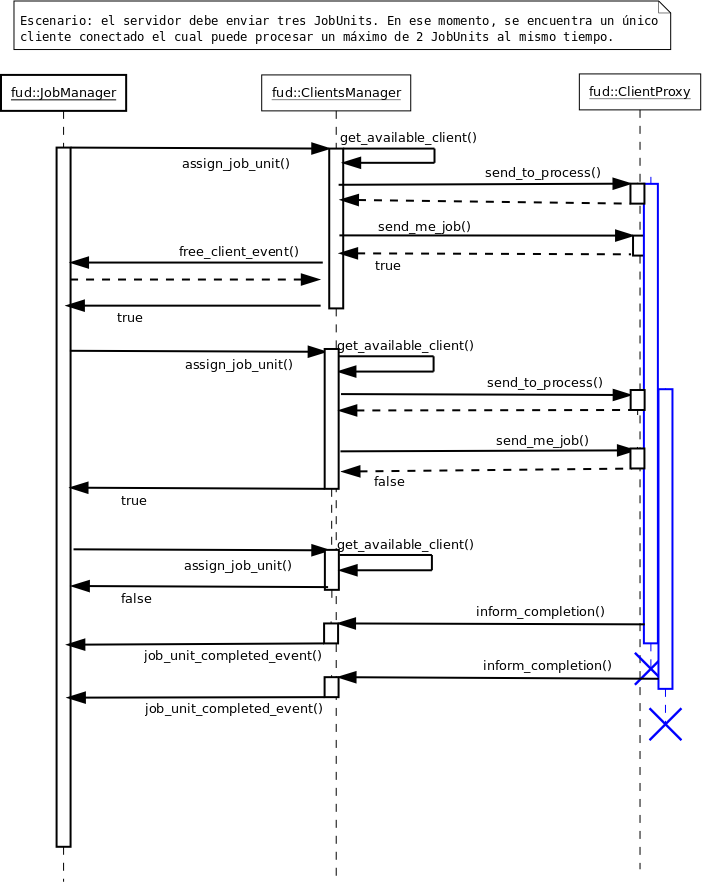
\includegraphics[scale=0.42]{redesing-multiplesJobs-on-client/assign_job_unit_seq_diagram.png}
		\caption{Diagrama de secuencia del rediseño de múltiples JobUnits a clientes}
		\label{fig:rediseno:diagram:seq:mult:jobs}
	\end{center}
\end{figure}


\newpage
\section{Métricas de código}

FuD-BOINC fue implementado en \texttt{7} archivos fuente los cuales suman un total de \texttt{1243} líneas de texto entre las que se distinguen líneas en blanco, comentarios y líneas de código. La tabla \ref{metrics:cloc} muestra un resumen de los resultados obtenidos al correr la aplicación \textit{Cloc} sobre los archivos de implementación de FuD-BOINC.

\begin{table}[!htf]
    \begin{center}
    \begin{tabular}{|l|r|r|r|r|c|}
    \hline
    \multicolumn{2}{|c|}{Files} & \multicolumn{3}{|c|}{Line Types} & \hspace{0.2cm}\% \\
    \hline
    \textbf{Type} & \textbf{Count} & \textbf{Blank} & \textbf{Comment} & \textbf{Source} & \small{\textbf{\#Comms./Tot.}}\\
    \hline
    \texttt{C++ source} & 2 &  130  &  120  &   466  &   20,47\\
    \hline
    \texttt{C++ header} & 5 &   95  &  292  &   140  &   67,59 \\
    \hline
    \textbf{Total} &    7   &  225  &  412  &   606  &   40,47 \\
    \hline
    \end{tabular}
    \caption{Resultados de CLOC para FuD-BOINC}
    \label{metrics:cloc}
    \end{center}
\end{table}

Podemos observar que de acuerdo a los resultados obtenidos, la capa de distribución FuD-BOINC no es un proyecto de gran tamaño. De un total de \texttt{1243} líneas escritas, sólo \texttt{606} líneas se corresponden a código fuente; un número relativamente bajo comparado con la complejidad del proyecto.

\textit{Dijkstra} escribió un interesante ensayo sobre por qué las industrias de software no deberían considerar las líneas de código como una medida exacta de la productividad del software o del programador. Mientras más líneas de código tenga, mayor es la complejidad de un producto de software, pero en el sentido de que es más difícil de mantener y entender; no tiene una relación directa con la funcionalidad que provee.

Otro resultado sorprendente que podemos observar en la tabla \ref{metrics:cloc} es el número de líneas de comentarios en el proyecto y su porcentaje con respecto al total de líneas de código efectivas del mismo:

$$\frac{\#comment\_lines}{\#comment\_lines + \#code\_lines}$$

Este valor es aproximadamente \texttt{0,40}, lo que indica que el \texttt{40\%} de las líneas de código se corresponden a líneas de comentarios. Este porcentaje se debe a que todos los archivos de implementación, por más chico que sea, poseen un header que ofrece ciertos detalles sobre el mismo, como sus autores, fecha de creación y la licencia por cual se rigen. En el código \ref{listing:fud:header} se puede ver el header que debe poseer cada archivo de código fuente.


\begin{lstlisting}[frame=shadowbox, language=C++, numbers=left, xleftmargin=8mm, framexleftmargin=22pt, basicstyle=\scriptsize, numberstyle=\footnotesize, breaklines=true, breakatwhitespace=false, caption={Header común en los archivos de implementación}, label=listing:fud:header, backgroundcolor=\color{gris}, firstnumber=170, tabsize=4, keywordstyle=\color{Blue}]
/**
*  \file:      boinc_clients_manager.h
*  \brief      Definition of BoincClientsManager class.
*              System:     FuD
*              Language:   C++
*
*  @author     Lucas Besso     -   E-Mail: lbesso AT gmail.com
*  @author     Raul Striglio   -   E-Mail: rulitox.s AT gmail.com
*
*
*  @Last Update:
*      $Id: boinc_clients_manager.h 850 2011-12-12 15:02:09Z lbesso $
*      $URL: https://fud.googlecode.com/svn/branches/boinc/src/middlewares/boinc/server/boinc_clients_manager.h $
*      $LastChangedBy: lbesso $ Author of last commit
*
*
* FuD is free software: you can redistribute it and/or modify
* it under the terms of the GNU General Public License as published by
* the Free Software Foundation, either version 3 of the License, or
* (at your option) any later version.
*
* FuD is distributed in the hope that it will be useful,
* but WITHOUT ANY WARRANTY; without even the implied warranty of
* MERCHANTABILITY or FITNESS FOR A PARTICULAR PURPOSE.  See the
* GNU General Public License for more details.
*
* You should have received a copy of the GNU General Public License
* along with FuD.  If not, see <http://www.gnu.org/licenses/>.
*/
\end{lstlisting}

Otro motivo que explica esta cantidad de líneas de comentarios es que todo componente de software tal como clases, estructuras, funciones, atributos, etc., tiene una descripción detallada a ser interpretada por Doxygen para la generación de automática de documentos. En el código \ref{listing:fud:doxygen} podemos observar un ejemplo de notación utilizando \texttt{doxygen}\footnote{\url{http://www.doxygen.org/}}.

\begin{lstlisting}[frame=shadowbox, language=C++, numbers=left, xleftmargin=8mm, framexleftmargin=22pt, basicstyle=\scriptsize, numberstyle=\footnotesize, breaklines=true, breakatwhitespace=false, caption={Ejemplo de comentario Doxygen utilizado en FuD-BOINC}, label=listing:fud:doxygen, backgroundcolor=\color{gris}, firstnumber=170, tabsize=4, keywordstyle=\color{Blue}]
            /** 
            * Create the boinc workunit to be computed.
            *
            *   @param name_input_file : The workunit's inputfile name
            *   @param wu_template : The BOINC's workunit template
            */
            void create_boinc_work(std::string name_input_file, const char* wu_template) throw (BoincWorkException);
\end{lstlisting}

En el apéndice \ref{chapter:FuD-BOINC:metrics_report} podemos encontrar un reporte completo sobre las métricas de código generado con la aplicación \texttt{cccc}\footnote{\url{http://cccc.sourceforge.net/}}. Éste incluye varias métricas de diseño orientado a objetos y todo tipo de información relevante en lo que respecta al código.

\subsection{Cobertura de código}

La cobertura de código es una medida utilizada en pruebas de software. Ésta describe el grado en que el código fuente de un programa ha sido testeado. Para FuD-BOINC se ejecutó la prueba de cobertura de código mediante la aplicación \texttt{GCov}\footnote{\url{http://gcc.gnu.org/onlinedocs/gcc/Gcov.html}}.

En la tabla \ref{table:gcov:server} se muestra la cobertura de código de los archivos que implementan el lado servidor de FuD-BOINC y en la tabla \ref{table:gcov:client} se muestra la cobertura de código de los archivos que implementan el lado cliente de FuD-BOINC.

\begin{table}[H]
    \begin{center}
    \begin{tabular}{|l|r|r|c|}
        \hline
        & \multicolumn{2}{|c|}{Líneas de código} & Porcentaje \\
        \hline
        \textbf{Archivo} & \textbf{Total} & \textbf{Ejecutado} & \hspace{0.2cm}\textbf{\%} \\
        \hline
        \scriptsize{boinc\_constants.h} & 4 & 4 & 100 \\
        \hline 
        \scriptsize{boinc\_clients\_manager.cpp} & 240 & 163 & 67.9 \\
        \hline 
        \scriptsize{boinc\_client\_manager.h} & 15 & 9 & 60 \\
        \hline 
        \scriptsize{boinc\_exception.h} & 4 & 0 & 0 \\
        \hline 
    \end{tabular}
    \caption{Resultados de cobertura para los archivos de código del servidor FuD-BOINC}
    \label{table:gcov:server}
    \end{center}
\end{table}

\begin{table}[H]
    \begin{center}
    \begin{tabular}{|l|r|r|c|}
        \hline
        & \multicolumn{2}{|c|}{Líneas de código} & Porcentaje \\
        \hline
        \textbf{Archivo} & \textbf{Total} & \textbf{Ejecutado} & \hspace{0.2cm}\textbf{\%} \\
        \hline
        \scriptsize{boinc\_distribution.h} & 1 & 0 & 0.00 \\
        \hline 
        \scriptsize{boinc\_distribution.cpp} & 240 & 163 & 67.9 \\
        \hline 
        \scriptsize{boinc\_client\_manager.h} & 58 & 43,99 & 75.86 \\
        \hline 
        \scriptsize{boinc\_exception.h} & 2 & 0 & 0 \\
        \hline 
    \end{tabular}
    \caption{Resultados de cobertura para los archivos de código del cliente FuD-BOINC}
    \label{table:gcov:client}
    \end{center}
\end{table}


		\chapter{Pruebas}
\label{chapter:pruebas}

El desarrollo de software implica una serie de actividades de producción en donde las posibilidades de que aparezcan fallos humanos son muy probables. Los errores pueden empezar a darse desde el primer momento del proceso. Es por eso que el desarrollo de software debe ir acompañado de una actividad que garantice la calidad del mismo.

En este capítulo se presentan los distintos casos de prueba y aplicaciones implicadas en las correspondientes pruebas realizadas sobre FuD-BOINC.

\section{Aplicaciones de prueba}

Desde los comienzos y durante el desarrollo de este proyecto, se realizaron severas pruebas utilizando algunas aplicaciones ofrecidas por BOINC y FuDePAN. Dichas pruebas fueron aplicadas durante toda la fase de implementación, con el fin de reducir errores, mejorar la funcionalidad y detectar posibles fallas.

A continuación se realiza una breve descripción de las aplicaciones utilizadas.

\subsection{Aplicaciones uppercase y create-work}

BOINC provee de varias aplicaciones de ejemplo junto con su código fuente. Entre ellas se encuentra la aplicación \textbf{uppercase} la cual dado un archivo de entrada conteniendo texto en minúscula genera un archivo de salida con el texto traducido a mayúsculas. 

La aplicación fue utilizada durante el proceso de investigación para entender cómo trabaja BOINC desde adentro. Se analizó 
su código fuente y se la ejecutó sobre el proyecto BOINC para corroborar que este último funcionara correctamente.

Debido a que esta aplicación sólo fue desarrollada como cliente (sin contar con un servidor que genere trabajos), para la creación y envío de trabajos a la misma se debió hacer uso de la aplicación \texttt{create\_work} ofrecida por BOINC para ayudar a desarrolladores en las pruebas de sus aplicaciones. La aplicación \texttt{create work} permite crear \texttt{workunits} desde la línea de comandos manteniendo así el flujo constante de unidades de trabajo para una determinada aplicación.

Estas pruebas fueron claves para comprender desde adentro cómo funciona la creación de trabajos de BOINC. Además, a partir del código fuente de la aplicación \textbf{uppercase} se obtuvieron las primeras ideas y una estructura base que fueron necesarias en la etapa de diseño para poder desarrollar una solución para la integración de FuD y BOINC.


\subsection{Aplicación de juguete Counter}

Counter es una aplicación simple provista por FuD como aplicación de ejemplo junto con su código fuente. Su función es contar hasta un número N dado usando X contadores. La tarea de cada contador es incrementar en 1 el número recibido e informarlo al servidor. Por lo tanto, cada \texttt{JobUnit} encapsula un número que el contador debe incrementar.

Las primeras pruebas realizadas sobre FuD-BOINC se llevaron a cabo utilizando esta aplicación las cual permitió probar cada implementación parcial durante las primeras versiones de nuestro proyecto logrando así detectar errores y flaquezas de la nueva implementación.

\subsection{Aplicación Parallel-Clusterer}
\label{seccion:pruebas:clusterer}

\textbf{Clustering} o \textbf{Data Clustering:} es un método que permite crear grupos de ciertos objetos (clúster). Los objetos pertenecientes a un clúster son muy similares y los objetos de distintos clústers son muy diferentes.\\

\textbf{Parallel-clusterer:} es una aplicación desarrollada por la organización FuDePAN para realizar clustering de proteínas.\\ 

\textbf{Clustering de proteínas:} dado un conjunto de diferentes posibilidades geométricas de una sola proteína (cada una representada como un vector de átomos) agrupa estos elementos según una función de similitud en las posiciones de sus átomos. El resultado final es un conjunto de agrupaciones o clústers donde cada uno tiene proteínas cuya estructura geométrica es muy similar.

El conjunto que toma como entrada la aplicación es pasado a la misma mediante un archivo generado con la aplicación \textit{Backbone-Generator} explicada a continuación.\\

\textbf{Backbone-Generator:}\label{subsection:bbgen} el generador de backbones de proteínas busca proporcionar nuevas respuestas y/o soluciones a los inconvenientes y dificultades que surgen en la predicción de estructura de proteínas a partir de una secuencia de aminoácidos.

Esta aplicación toma como entrada un archivo con los pares de ángulos posibles a combinar y un número de residuos (conjunto de 3 átomos). pasado mediante el flag ``-r'' que indica la longitud del backbone resultante. Como salida, se genera un archivo resultado con una secuencia de átomos que representa el backbone o estructura de una proteína. Dependiendo de la cantidad de residuos y cantidad de pares de ángulos que tome la aplicación, el tamaño del archivo resultante puede llegar a ser extremadamente pesado debido a que sobre el mismo se escriben todas las posibles combinación entre los residuos y los pares de ángulos. Por ejemplo, la ejecución de la aplicación con 15 residuos (\texttt{-r15}) y cuatro pares de ángulos, generó un archivo con un tamaño de \texttt{160,3 MB}.


\section{Casos de prueba}

En esta sección se presentan los distintos casos de prueba realizados mediante el uso de las aplicaciones Counter y Parallel-clusterer compiladas con FuD-BOINC. 
El objetivo de estos casos de prueba consistió en testear las distintas versiones que se obtuvieron durante todo el desarrollo de este proyecto hasta la versión final del mismo.

A continuación se especifican las características del ordenador servidor y de las computadoras clientes que se utilizaron en las pruebas:

\textbf{\\Servidor:}\\

Las aplicaciones servidoras se ejecutaron siempre sobre una computadora con las siguientes características:

\begin{itemize}
 \item \textbf{Sistema Operativo}: Ubuntu 10.10 Maverick Meerkat(32 bits).
 \item \textbf{Procesador}: Intel Core i5
 \item \textbf{N° Núcleos del procesador}: 4
 \item \textbf{Memoria RAM}: 4Gb
 \item \textbf{Velocidad de conexión}: conexión hogareña de 3MB.
\end{itemize}

\textbf{\\Cliente:}\\

En cambio, las aplicaciones clientes fueron ejecutadas sobre ordenadores con las siguientes características:

\begin{itemize}
 \item \textbf{Sistemas Operativos}: Ubuntu 10.10(32 bits), Microsoft Windows XP (32 bits) y Windows 7 (32 bits).
 \item \textbf{Procesador}: Variaron entre modelos antiguos como es el Amd Athlon Xp 2000 a modelos más actuales como el Intel® Core™2 Duo Processor P8600.
 \item \textbf{N° Núcleos del procesador}: entre 1 y 2.
 \item \textbf{Memoria RAM:} entre 512MB y 3Gb.
 \item \textbf{Velocidad de conexión}: conexiones hogareñas entre 256Kbps y 3MB.
\end{itemize}


\subsection{Funcionamiento de Counter con FuD-BOINC}

El Counter es una aplicación pequeña la cual no requiere demasiados recursos de red y procesamiento debido a que simplemente se envía un número como contenido de cada tarea para que éste sea incrementado en uno por el cliente. Por dicho motivo, se optó por utilizarla para realizar las pruebas iniciales del desarrollo donde se crearon los casos de prueba detallados a continuación.

\subsubsection{Verificar envío y recepción de trabajos}
Esta prueba consistió en ejecutar la aplicación Counter compilada con FuD-BOINC sobre un proyecto BOINC con el fin de verificar la correctitud del servidor a la hora de enviar trabajos al cliente, y del cliente a la hora de computar tareas y devolver resultados al servidor.

Mediante esta prueba se pudo detectar que la aplicación servidora en ningún momento generaba trabajos debido a que no se efectuaba la registración del cliente en el servidor. La solución a dicho problema derivó en un rediseño de la capa de manejo de trabajos de FuD explicado en la sección \ref{seccion:jobmanager:post:init}. Luego de aplicar la correspondiente solución al problema, se volvió a realizar este caso de prueba y la aplicación funcionó correctamente.

\subsubsection{Ejecutar cliente sobre Microsoft Windows} 
Esta prueba consistió en compilar la aplicación Counter para plataformas Windows y correr un cliente BOINC sobre este sistema operativo con el fin de evaluar su funcionamiento. Por lo tanto, por un lado se ejecutó la aplicación servidora del Counter sobre un proyecto BOINC, y por el otro se conectó al proyecto con un cliente Windows. 

Mediante esta prueba detectamos un error por linkeo de librerías dinámicas. Es decir, que en el momento que el \texttt{BOINC Manager} intentó ejecutar la aplicación cliente del Counter, ésta falló por no encontrar las librería necesarias instaladas en dicho sistema operativo. 

Cabe destacar, que este problema no había sido detectado en Linux ya que la implementación y ejecuciones, tanto del servidor como del cliente, eran realizadas en el mismo ordenador el cual contenía instaladas todas las librerías requeridas.

Para solucionar este problema se debió compilar la aplicación cliente con linkeo estático de librerías tanto para Linux como para Windows.

Luego de resolver este problema, se volvieron a realizar las pruebas con clientes conectados desde Windows y Linux en donde no se detectaron nuevas fallas. Es decir, que en esta instancia, la aplicación Counter compilada con FuD-BOINC quedó funcionando correctamente.


\subsection{Funcionamiento de Parallel-Clusterer con FuD-BOINC}

Las pruebas más relevantes sobre FuD-BOINC se realizaron utilizando la aplicación Parallel-Clusterer debido a que ésta envía información más grande que un simple número como es el caso de la aplicación Counter. Mediante dichas pruebas se pudo chequear de manera completa la interacción \texttt{cliente-servidor} de FuD-BOINC. 

Del lado servidor, las pruebas se focalizaron en la creación de nuevos trabajos y en la asimilación de resultados (\ref{seccion:asimilador}). 

Por el contrario, del lado cliente las pruebas se focalizaron en la lectura e interpretación del archivo de entrada y en la escritura de los resultados en el archivo de salida. 

Debemos destacar que el objetivo de estas pruebas consistió en complementar las pruebas realizadas con la aplicación Counter. Por ello, se crearon varios casos de prueba detallados a continuación.

\subsubsection{Ejecutar Parallel-Clusterer con FuD-BOINC}

Esta prueba tuvo como único objetivo probar una nueva aplicación compilada sobre FuD-BOINC con el fin de chequear que el correcto funcionamiento obtenido, luego de probar la aplicación Counter, se seguía manteniendo.

En esta instancia, se detectó que la capa L2 de FuD sólo entregaba de a dos trabajos, problema que motivó el rediseño de la capa L2 de FuD explicada en la sección \ref{seccion:multiples:jobunits:clientes} de este informe. 

Luego de aplicar la correspondiente solución al problema, la aplicación Parallel-Clusterer funcionó correctamente enviando más de un trabajo a cada cliente BOINC conectado al proyecto.

\subsubsection{Ejecutar Parallel-Clusterer sobre Microsoft Windows}

Una de los casos de pruebas que se realizó para esta aplicación, consistió en ejecutarla con un cliente conectado desde Linux y un cliente conectado desde Windows. A partir de esta prueba, se descubrió que la aplicación cliente corriendo sobre Windows generaba un error al intentar leer el archivo de entrada que recibía desde el servidor.

Para descubrir la causa por la que se generaba este error, se escribió una aplicación de prueba que realizaba los mismos pasos para la lectura del archivo que se llevaba a cabo en la aplicación cliente. El test fue compilado y ejecutado tanto en Linux como en Windows produciéndose el mismo error comentado. 

El código \ref{listing:test:binary:file} muestra la implementación de la aplicación de prueba.

\begin{lstlisting}[frame=shadowbox, language=C++, numbers=left, xleftmargin=8mm, framexleftmargin=22pt, basicstyle=\scriptsize, numberstyle=\footnotesize, breaklines=true, breakatwhitespace=false, caption={Test de lectura realizada por un cliente FuD-BOINC}, label=listing:test:binary:file, backgroundcolor=\color{gris}, keywordstyle=\color{Blue}]
#include <iostream>
#include <string>
#include <vector>
#include "mili/mili.h"
#include <fstream>

typedef mili::bistream InputMessage;
typedef uint32_t      JobUnitID;

int main(int argc, char** argv)
{
    JobUnitID _current_id;

    std::clog << "FuD: starting FuD computation." << std::endl;
       
    std::string file_name(argv[1]);
    std::ifstream ifs(file_name.c_str(), std::ios::binary);
//    std::ifstream ifs(file_name.c_str()); Linea original reemplazada por el anterior

    // Enable file exceptions.
    ifs.exceptions(std::ifstream::eofbit | std::ifstream::failbit | std::ifstream::badbit);

    std::clog << "FuD: extracting the input file for computation." << std::endl;
        
    // Extract the content of the input file to deliver.
    std::stringstream oss;
    oss << ifs.rdbuf();
    InputMessage input_msg (oss.str() );

    // Get the message and _current_id
    std::string message;
    input_msg >> _current_id >> message;
    
    std::clog << "FuD: id=" << _current_id << std::endl;
    std::clog << "FuD: message=" << message.c_str() << "FIN" << std::endl;

    ifs.close();
    std::clog << "FuD: exit." << std::endl;

    exit(0);
}
\end{lstlisting}

\hspace{2mm}

\textbf{Causa del error:} la causa de este error, se debió a que Windows diferencia la manera en que maneja los archivos de texto y los binarios, mientras que Linux los trata a todos como binarios. Por consiguiente, el servidor de FuD-BOINC envíaba un archivo binario mientras que el cliente FuD-BOINC lo intentaba leer como archivo de texto causando así el error de lectura del mismo. 

\textbf{Solución:} simplemente se debió especificar el tipo de fichero a escribir y a leer tanto en el servidor como en el cliente, agregando el flag \texttt{std::ios::binary} a la operación \texttt{open} del archivo. Este cambio primero se corroboró en el código \ref{listing:test:binary:file} agregando el flag mencionado en la línea 17.

Para finalizar, se efectuaron diversas pruebas utilizando clientes BOINC corriendo sobre diferentes distribuciones Windows en donde no se encontraron nuevas fallas. Se obtuvo así una versión estable y final de FuD-BOINC.


		\chapter{Resultados}
\label{chapter:resultados}

\section{Análisis de Rendimiento}

Es importante realizar el análisis de rendimiento de una aplicación distribuida con el propósito de estudiar los beneficios que ésta posee ante la comparación con su versión secuencial. 
Al desarrollar un programa distribuido no solo se intenta alcanzar el mejor rendimiento del mismo sino que también se intenta mantenerlo en proporción, a medida que se añaden nuevos nodos de procesamiento.

En el caso de una aplicación secuencial, ésta es usualmente evaluada en términos de su tiempo de ejecución expresado como una función de su tamaño de entrada. El tiempo de ejecución de un programa distribuido no sólo es evaluado en términos del tamaño de la entrada sino que también influyen otros factores tales como el número de nodos de procesamiento que posee y el coste de comunicación entre dichos nodos.

A continuación se muestra el análisis de rendimiento de la aplicación Parallel-Clusterer en términos de las métricas principales calculadas sobre este programa, tales como  \textit{aceleración, eficiencia, overhead} y \textit{costo}. La ejecución se llevo a cabo con un archivo de entrada generado con 9 residuos, variando de 1 a 5 clientes conectados.\\

\subsection{Tiempo de ejecución}

El tiempo de ejecución de un programa se define como el intervalo de tiempo que transcurre desde que el programa se inicia hasta que finaliza. En el caso de un programa distribuido, éste se calcula desde que se inicia el mismo hasta que el último nodo finaliza su ejecución.

Se denotará el tiempo secuencial que toma la aplicación como \textit{T$_{s}$} y el tiempo distribuido como \textit{T$_{p}$}. El promedio de \textit{T$_{s}$} luego de 10 ejecuciones de la aplicación Parallel-Clusterer fue de 110.7 segundos.

En la figura \ref{ts_vs_tp} se muestran los tiempos de ejecución promedio para cinco clientes así como su comparación con el algoritmo secuencial. Podemos observar sobre dicha figura que, con solo 5 nodos, los tiempos de procesamiento que toma la solución distribuida no es más óptima respecto de la solución secuencial. Sin embargo, es fácil ver que el tiempo va disminuyendo considerablemente a medida que se agregan nodos de procesamiento. Estos resultados variaron por diversos factores más allá del coste de comunicación y de la cantidad de nodos:

\begin{itemize}

  \item \textit{descarga de trabajos:} los trabajos de entrada que recibe cada cliente pesaron entre 60kb y 390kb. El tiempo tomado por cada cliente en descargar los trabajos en relación con su velocidad de conexión obviamente afectó directamente al tiempo total de la aplicación.

  \item \textit{subir resultados al servidor:} los resultados generados son escritos en un archivo de salida para que luego cada cliente BOINC los suba al servidor del proyecto. En este caso, el tiempo que tardó un cliente en subir dicho archivo, en relación con su velocidad de conexión, influyó también en el tiempo total de la aplicación.

  \item \textit{tiempo entre requerimientos:} la aplicación \textit{BOINC Manager}, nombrada en la sección \ref{boinc:manager}, envía requerimientos de nuevas tareas al servidor cada X cantidad de tiempo (X representa segundos e incluso minutos). Por ejemplo, en estas pruebas, el cliente envió requerimientos al servidor instantáneamente después de reportar una tarea. Si mediante éstos no obtuvo nuevos trabajos, esperaba entre 1 y 2 minutos para volver a requerir. Esto último es un factor negativo para el tiempo final.

\end{itemize}
\label{factores:tiempo}

\begin{center}
\begin{figure}[!ht]
    %Tabla & Grafico
    \begin{minipage}{2,5cm}
    \begin{flushleft}
    \begin{tabular*}{2,0cm}{c@{\extracolsep{\fill}}c}
        \hline
        \textbf{p} & \textbf{$T_p$} \\ \hline 
        1 & 305 \\ \hline
        2 & 249 \\ \hline
        3 & 259 \\ \hline
        4 & 245 \\ \hline
        5 & 222 \\ \hline
    \end{tabular*}
    \end{flushleft}
    \end{minipage}
    \    \ \hfill
    \begin{minipage}{12cm}
    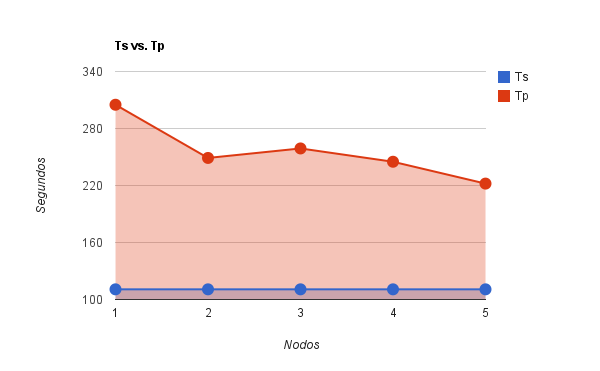
\includegraphics[scale=0.6]{images/Grafico_de_tiempos.png}\\
    \end{minipage}
    \caption{Tiempo secuencial vs. paralelo}
    \label{ts_vs_tp}
\end{figure}
\end{center}

Haciendo un análisis de la comparación que se observa en el gráfico \ref{ts_vs_tp}, y considerando que las \texttt{JobUnits} generadas por la aplicación en estas pruebas pesaron como máximo aproximada \texttt{400kb}, se podría pensar en una nueva versión del Parallel-Clusterer pensada para trabajar con FuD-BOINC en donde cada \texttt{JobUnit} demore mucho más en procesarse aumentando la cantidad de instrucciones efectuadas por un cliente con el fin de reducir la cantidad de requerimientos generados por los clientes.


\subsection{Aceleración}

Es una medida que arroja el beneficio relativo de resolver un problema en paralelo. Ésta es definida como la relación del tiempo que toma resolver un problema en un sólo procesador con el tiempo requerido para resolverlo en una arquitectura paralela con \textit{n} nodos de procesamiento idénticos. Se denota con el símbolo \textit{S} y se define como
\textit{S} = \textit{T$_{s}$}/\textit{T$_{p}$}

\begin{center}
\begin{figure}[!ht]
    %Tabla & Grafico
    \begin{minipage}{2,5cm}
    \begin{flushleft}
    \begin{tabular*}{2,0cm}{c@{\extracolsep{\fill}}c}
        \hline
        \textbf{p} & \textbf{$S$} \\ \hline 
        1  & 0.36 \\ \hline
        2  & 0.44 \\ \hline
        3  & 0.42 \\ \hline
        4  & 0.45 \\ \hline
        5  & 0.49 \\ \hline
    \end{tabular*}
    \end{flushleft}
    \end{minipage}
    \    \ \hfill
    \begin{minipage}{12cm}
    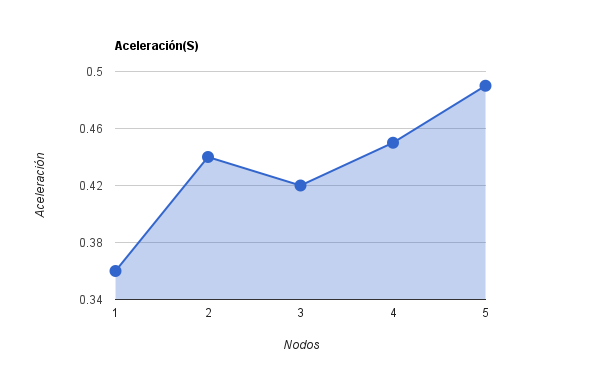
\includegraphics[scale=0.6]{images/Grafico_Aceleracion.png}\\
    \end{minipage}
    \caption{Aceleración}
    \label{speedup}
\end{figure}
\end{center}

En la figura \ref{speedup} podemos observar que no hay un crecimiento ``lineal'' de la aceleración. Se puede ver que para 2 nodos la aceleración mejora respecto del valor obtenido con 3 nodos. Este caso se debe a los factores explicados anteriormente, donde evidentemente en la ejecución con 3 nodos afectaron más que en el resto de los casos. Sacando ese caso particular, se observa que la aceleración crece a medida que se agregan más nodos de procesamiento. Ésto se debe a que al aumentar la cantidad de nodos disponibles, aumenta la cantidad de requerimientos provocando que las tareas sean asignadas más rápido a los clientes.

\subsection{Eficiencia}

La eficiencia de un programa paralelo indica la fracción de tiempo útil de un elemento de procesamiento. 
Se define como: \textit{E} = \textit{S}/\textit{p}

\begin{center}
\begin{figure}[H]
    %Tabla & Grafico
    \begin{minipage}{2,5cm}
    \begin{flushleft}
    \begin{tabular*}{2,0cm}{c@{\extracolsep{\fill}}c}
        \hline
        \textbf{p} & \textbf{$E$} \\ \hline 
        1  & 0.36 \\ \hline
        2  & 0,22 \\ \hline
        3  & 0,14 \\ \hline
        4  & 0,11 \\ \hline
        5  & 0,09 \\ \hline
    \end{tabular*}
    \end{flushleft}
    \end{minipage}
    \    \ \hfill
    \begin{minipage}{12cm}
    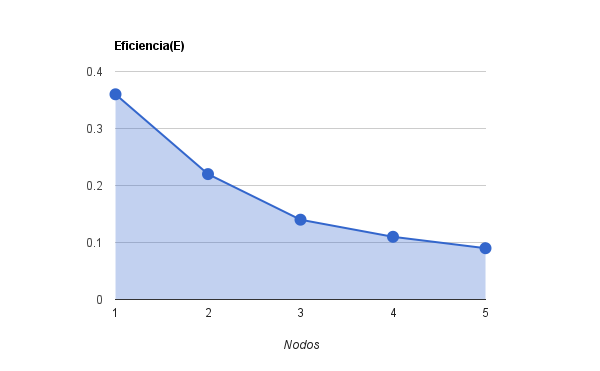
\includegraphics[scale=0.5]{images/Grafico_Eficiencia.png}\\
    \end{minipage}
    \caption{Eficiencia}
    \label{eficiency}
\end{figure}
\end{center}

En la figura \ref{eficiency}, vemos que la función de eficiencia decae, lo que significa una utilidad nodal inversamente proporcional a la cantidad de nodos de procesamiento. Ésto deja en claro que a mayor cantidad de nodos, más decae la eficiencia.


\subsection{Overhead}

El overhead de un programa paralelo es el trabajo adicional que dicho programa realiza respecto a la solución secuencial equivalente y se define como:

\textit{T$_{o}$} = \textit{p} ∗ \textit{T$_{p}$} − \textit{T$_{s}$}

\begin{center}
\begin{figure}[H]
    %Tabla & Grafico
    \begin{minipage}{2,5cm}
    \begin{flushleft}
    \begin{tabular*}{2,0cm}{c@{\extracolsep{\fill}}c}
        \hline
        \textbf{p} & \textbf{$T_0$} \\ \hline 
        1  & 194.3 \\ \hline
        2  & 387.3 \\ \hline
        3  & 666.3 \\ \hline
        4  & 869.3 \\ \hline
        5  & 999.3 \\ \hline
    \end{tabular*}
    \end{flushleft}
    \end{minipage}
    \    \ \hfill
    \begin{minipage}{12cm}
    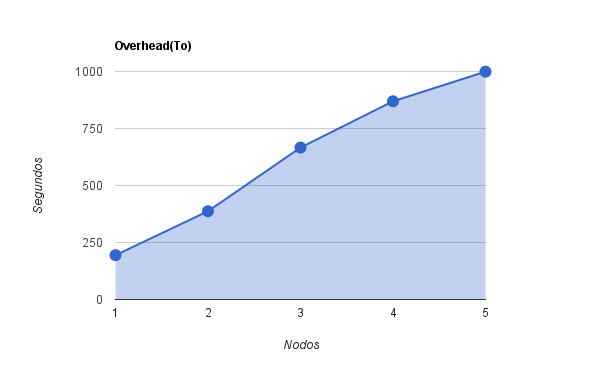
\includegraphics[scale=0.6]{images/Grafico_Overhead.png}\\
    \end{minipage}
    \caption{Overhead}
    \label{overhead}
\end{figure}
\end{center}

En la figura \ref{overhead}, vemos que el overhead aumenta a medida que se agregan nodos de procesamiento, lo que indica una suma de trabajo adicional por cada nuevo nodo de procesamiento. En el caso de FuD-BOINC, este trabajo adicional que agrega cada cliente se debe a un aumento de la cantidad de requerimientos que debe atender el servidor.

\subsection{Costo}

El costo de un programa paralelo refleja la suma de los tiempos de ejecución de cada proceso, y se define como:
 \textit{C} = \textit{p} ∗ \textit{T$_{p}$} . Se dice que un programa paralelo tiene costo óptimo si tiene costo computacional igual al programa secuencial.

\newpage
\begin{center}
\begin{figure}[!ht]
    \begin{minipage}{2,5cm}
    \begin{flushleft}
    \begin{tabular*}{2,0cm}{c@{\extracolsep{\fill}}c}
        \hline
        \textbf{p} & \textbf{$C$} \\ \hline 
        1  & 305 \\ \hline
        2  & 498 \\ \hline
        3  & 777 \\ \hline
        4  & 980 \\ \hline
        5  & 1110 \\ \hline
    \end{tabular*}
    \end{flushleft}
    \end{minipage}
    \    \ \hfill
    \begin{minipage}{12cm}
    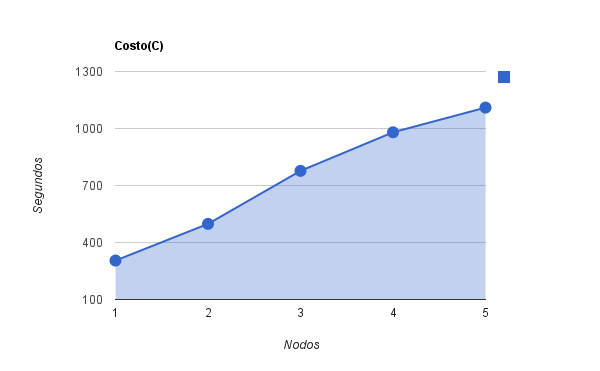
\includegraphics[scale=0.6]{images/Grafico_Costo.png}\\
    \end{minipage}
    \caption{Costo}
    \label{cost}
\end{figure}
\end{center}

En la figura \ref{cost} se observa que el costo tiene una curva similar al overhead. En este gráfico se muestra un costo directamente proporcional a la cantidad de nodos participantes.

\section{FuD-BOINC Vs FuD-Asio}

En esta sección se presenta una comparación de los resultados obtenidos de ejecutar la aplicación Parallel-Clusterer (\ref{seccion:pruebas:clusterer}) compilada con las librerías FuD-BOINC y FuD original (FuD-Asio). El objetivo de esta comparación consiste en poder verificar que los resultados de ambas pruebas sean iguales o aproximados con el fin de poder contar con resultados que garanticen que el diseño e implementación de FuD-BOINC siguen manteniendo el modelo que ofrece el diseño de original de FuD.

Debemos destacar que dicha aplicación genera resultados no determinísticos. Ésto se debe a la forma en que se eligen los representantes de cada clúster resultante. Por ejemplo, al principio de la computación se envían a los clientes \texttt{JobUnits} para armar un conjunto de representantes a partir de los cuales se van a construir los clusters. En cada ejecución, podría ocurrir que los clientes retornen los resultados\footnote{Un representante para la creación de un clúster} en distinto orden respecto del \texttt{ID} que posee la \texttt{JobUnit} asignada a cada uno. De esta manera, los resultados finales  podrían variar por cada ejecución ya que los representantes utilizados para comenzar a crear cada clúster podrían llegar en distinto orden. \\

Para la obtención de resultados, se tomaron como casos de prueba la ejecución de la aplicación Parallel-Clusterer pasándole como entrada archivos generados con 5,6,7,8 y 9 residuos comparando la cantidad de clusters obtenidos. El cuadro \ref{Fb_vs_fa} muestra los valores obtenido por cada ejecución. La columna \textit{residuos} indica la cantidad de residuos con los que se generó el archivo de entrada que se utilizó para esa prueba. Las columnas \textit{``N° Clusters con FuD-BOINC''} y \textit{``N° Clusters con FuD-Asio''} muestran la cantidad de clústers obtenidos en la ejecución de la aplicación utilizando la librería FuD-BOINC y FuD-Asio respectivamente.\\

\begin{table}[H]
\begin{center}
\begin{tabular}{| c| c| c| c|}
\hline
\textbf{Residuos} & \textbf{N° Clusters con FuD-BOINC} & \textbf{N° Clusters con FuD-Asio}\\ \hline 
5  & 11 & 11 \\ 
\hline
6  & 50 & 50 \\ 
\hline
7  & 155 & 155 \\ 
\hline
8  & 384 & 384 \\ 
\hline
9  & 1023 & 1023 \\ 
\hline
\end{tabular}
\caption{Comparación de resultados Parallel-Clusterer}
\label{Fb_vs_fa}
\end{center}
\end{table}

Considerando que las pruebas se realizaron utilizando una aplicación compleja como es el Parallel-Clusterer y que en los resultados plasmados en el cuadro \ref{Fb_vs_fa} la cantidad de clústers obtenidos son equivalentes en todas las pruebas realizadas, se puede decir que el comportamiento de dicha aplicación utilizando la capa de distribución FuD-BOINC fue el esperado.
	\part{Conclusión}\label{conclusion}
		\chapter{Conclusión}
\label{chapter:conclusion}

Gracias a las tareas realizadas a lo largo de este proyecto, se han obtenido diferentes resultados; algunos positivos y otros no tan alentadores. Sin embargo, la evaluación final resulta ser muy positiva debido a que todas las metas propuestas al comienzo del proyecto fueron cumplidas satisfactoriamente.

En principio se logró implementar la nueva capa de distribución FuD-BOINC manteniendo la compatibilidad con las aplicaciones que actualmente utilizan al modelo original de FuD.

En segundo lugar, realizando un análisis de los resultados obtenidos tanto de las pruebas efectuadas con la aplicación \textit{Counter} como con \textit{Parallel Clusterer}, se puede afirmar que la implementación de FuD-BOINC junto con los rediseños llevados a cabo sobre FuD no afectan al modelo propuesto por el mismo, ni a su correcto funcionamiento. De esta manera, los desarrolladores que utilicen a FuD en sus implementaciones pueden variar de una capa de distribución a otra con la certeza de que los resultados obtenidos al ejecutar sus aplicaciones serán realmente los esperados.

Como tercer punto, se logró compilar la aplicación cliente de \textit{Parallel Clusterer} para que pueda correr sobre sistemas Windows suministrando así una configuración base la cual servirá de guía para la compilación de futuras aplicaciones FuD que necesiten correr sobre este sistema operativo mediante el middleware BOINC.

Por último, basándose de los resultados obtenidos en el análisis de rendimiento de una aplicación compilada con FuD-BOINC, donde sus JobUnits no requieren gran cantidad de procesamiento para su computación, se puede afirmar que el tiempo total de ejecución en general, serán más elevados que su solución secuencial cuando la cantidad de voluntarios sea muy reducida. Esto se debe a cómo funciona BOINC en la distribución de sus trabajos, la cual se basa en requerimientos de tareas por parte de clientes, efectuados en intervalos de tiempos variables. Por el contrario, si la cantidad de voluntarios es elevada, los tiempos entre cada requerimiento de tarea recibidos por el servidor será mínimo por lo que las tareas serán distribuidas rápidamente. A su vez, el paralelismo en este caso sería aún mayor.
		\chapter{Trabajos a futuro}
\label{chapter:future:work}

La conclusión de este proyecto abre las puertas a FuDePAN al mundo de la computación voluntaria por lo que es importante avanzar sobre ciertos puntos. Es por ello que a continuación se presentará una lista de trabajos a futuro y funcionalidades extras para este proyecto, que serán dejadas como futuras tareas de la fundación:

\begin{itemize}
\item Instruir y profundizar los conocimientos sobre la administración y configuración de un proyecto BOINC con el fin de lanzar oficialmente un proyecto de computación voluntaria, \textbf{FuDePAN@HOME}, en donde se puedan ejecutar aquellas aplicaciones desarrolladas con FuD-BOINC.

\item Implementar las tareas de validación de resultados como un método específico de FuD-BOINC de tal manera que se pueda realizar validación de resultados redundantes en caso de que la aplicación lo requiera.

\item Extender el rediseño de múltiple jobs presentado en la sección \ref{seccion:multiples:jobunits:clientes} para que el lado cliente de la capa aplicación (L3) sea quien determine la cantidad de trabajos simultáneos que puede recibir.

\item Implementar un screensaver con un logo personalizado de FuDePAN utilizando la API de BOINC para que, al colaborar, cada voluntario pueda observar diferentes detalles de sus trabajos.

\item Agregar la entrega de créditos a los clientes respecto de la cantidad de trabajos procesados.

\end{itemize}

		
	% Bibliografia
	\part{Bibliografía}
	\label{biblio}
	    \nocite{*}
	    \addcontentsline{toc}{chapter}{Bibliografía}
	    \bibliography{Bibliografia}
	    \bibliographystyle{annotate}

    \part{Apéndices}
        \appendix \label{appendix}
        %\addappheadtotoc
        %\appendixpage
        %\newpage
        \chapter{Reporte de métricas de código de FuD-BOINC}
\label{chapter:FuD-BOINC:metrics_report}

\begin{tabular}{|c|l|}
\hline
\multicolumn{2}{|c|}{CCCC Software Metrics Report generated Tue Nov 22 20:34:56 2011} \\
 \hline 
 \textbf{Project}       & Summary table of high level measures summed over all\\
 \textbf{Summary}       & files processed in the current run.  \\
 \hline 
 \textbf{Procedural}    & Table of procedural measures (i.e. lines of code, \\
 \textbf{Metrics}       & lines of comment, McCabe's cyclomatic complexity \\
 \textbf{Summary}       & summed over each module.  \\
 \hline 
 \textbf{Object Oriented} & Table of four of the 6 metrics proposed by Chidamber \\
 \textbf{Design}        & and Kemerer in their various papers on 'a metrics suite \\
                        & for object oriented design'. \\
 \hline 
 \textbf{Structural}    & Structural metrics based on the relationships of each \\
 \textbf{Metrics}       & module with others. Includes fan-out (i.e. number of \\
 \textbf{Summary}       & other modules the current module uses), fan-in (number \\
                        & of other modules which use the current module), and \\
                        & the Information Flow measure suggested by Henry and \\
                        & Kafura, which combines these to give a measure of \\
                        & coupling for the module. \\
 \hline 
 \textbf{Other Extents} & Lexical counts for parts of submitted source files which \\
                        & the analyser was unable to assign to a module. Each \\
                        & record in this table relates to either a part of the \\
                        & code which triggered a parse failure, or to the residual \\
                        & lexical counts relating to parts of a file not \\
                        & associated with a specific module. \\
 \hline 
 \textbf{About CCCC}    & A description of the CCCC program.  \\
 \hline 
\end{tabular}
\newpage

\section{Project Summary}
 This table shows measures over the project as a whole. \begin{itemize}
\item NOM = Number of modules\\ 
 Number of non-trivial modules identified by the analyser. Non-trivial modules include all classes, and any other module for which member
functions are identified. 
\item LOC = Lines of Code\\ 
 Number of non-blank, non-comment lines of source code counted by the analyser. 
\item COM = Lines of Comments\\ 
 Number of lines of comment identified by the analyser 
\item MVG = McCabe's Cyclomatic Complexity\\ 
 A measure of the decision complexity of the functions which make up the program.The strict definition of this measure is that it is the
number of linearly independent routes through a directed acyclic graph which maps the flow of control of a subprogram. The analyser counts
this by recording the number of distinct decision outcomes contained within each function, which yields a good approximation to the formally
defined version of the measure. 
\item L\_C = Lines of code per line of comment\\ 
 Indicates density of comments with respect to textual size of program 
\item M\_C = Cyclomatic Complexity per line of comment\\ 
 Indicates density of comments with respect to logical complexity of program 
\item IF4 = Information Flow measure\\ 
 Measure of information flow between modules suggested by Henry and Kafura. The analyser makes an approximate count of this by counting
inter-module couplings identified in the module interfaces. 

\end{itemize}
 Two variants on the information flow measure IF4 are also presented, one (IF4v) calculated using only relationships in the visible part of
the module interface, and the other (IF4c) calculated using only those relationships which imply that changes to the client must be
recompiled of the supplier's definition changes. 

\begin{tabular}{|c|c|c|c|}
\hline 
Metric &Tag &Overall &Per Module \\
 \hline 
Number of modules &NOM & 16 &  \\
 \hline 
Lines of Code &LOC & 531 & 33.187 \\

 \hline 
McCabe's Cyclomatic Number &MVG & 34 & 2.125 \\

 \hline 
Lines of Comment &COM & 327 & 20.437 \\ 

 \hline 
LOC/COM &L\_C & 1.624 &  \\
 \hline 
MVG/COM &M\_C & 0.104 &  \\
 \hline 
Information Flow measure (  inclusive ) &IF4 & 0 & 0.000 \\
 \hline 
Information Flow measure (  visible ) &IF4v & 0 & 0.000 \\
 \hline 
Information Flow measure (  concrete ) &IF4c& 0 & 0.000 \\
 \hline 
Lines of Code rejected by parser &REJ & 40 &  \\
 \hline 

\end{tabular}



\section{Procedural Metrics Summary}
 For descriptions of each of these metrics see the information preceding the project summary table. The label cell for each row in this
table provides a link to the functions table in the detailed report for the module in question\\

\begin{tabular}{|c|c|c|c|c|c|}
\hline 
Module Name &LOC &MVG &COM &L\_C &M\_C \\
 \hline 
 BoincClientProxy & 290 & 23 & 41 & 7.073 & 0.561\\
 \hline 
 BoincClientsManager & 65 & 6 & 23 & 2.826 & 0.261  \\
 \hline 
 BoincDistribution & 96 & 3 & 41 & 2.341 & ------ \\
 \hline 
 BoincExceptionHierarchy & 1 & 0 & 5 & ------ & ------\\
 \hline 
 ClientsManager & 0 & 0 & 0 &------ &------ \\
 \hline 
 DB\_APP & 0 & 0 & 0 &------ &------ \\
 \hline 
 DB\_CONN & 0 & 0 & 0 &------ &------ \\
 \hline 
 DB\_RESULT & 0 & 0 & 0 &------ &------ \\
 \hline 
 DB\_WORKUNIT & 0 & 0 & 0 &------ &------ \\
 \hline 
 DistributionClient & 0 & 0 & 0 &------ &------ \\
 \hline 
 FILE\_INFO & 0 & 0 & 0 &------ &------ \\
 \hline 
 JobUnit & 0 & 0 & 0 &------ &------ \\
 \hline 
 boinc\_db & 0 & 0 & 0 &------ &------ \\
 \hline 
 bool & 0 & 0 & 0 &------ &------ \\
 \hline  
 string & 0 & 0 & 0 &------ &------ \\
 \hline 


\end{tabular}

\section{Object Oriented Design}
\begin{itemize}
\item WMC = Weighted methods per class\\ 
 The sum of a weighting function over the functions of the module. Two different weighting functions are applied: WMC1 uses the nominal
weight of 1 for each function, and hence measures the number of functions, WMCv uses a weighting function which is 1 for functions
accessible to other modules, 0 for private functions. 
\item DIT = Depth of inheritance tree\\ 
 The length of the longest path of inheritance ending at the current module. The deeper the inheritance tree for a module, the harder it may
be to predict its behaviour. On the other hand, increasing depth gives the potential of greater reuse by the current module of behaviour
defined for ancestor classes. 
\item NOC = Number of children\\ 
 The number of modules which inherit directly from the current module. Moderate values of this measure indicate scope for reuse, however
high values may indicate an inappropriate abstraction in the design. 
\item CBO = Coupling between objects\\ 
 The number of other modules which are coupled to the current module either as a client or a supplier. Excessive coupling indicates weakness
of module encapsulation and may inhibit reuse. 

\end{itemize}
 The label cell for each row in this table provides a link to the module summary table in the detailed report for the module in question\\

\begin{tabular}{|c|c|c|c|c|c|}
\hline 
Module Name &WMC1 &WMCv &DIT &NOC &CBO \\
 \hline 
 BoincClientProxy & 15 & 0 & 0 & 0 & 7 \\
 \hline 
 BoincClientsManager & 7 & 4 & 1 & 0 & 2 \\
 \hline 
 BoincDistribution & 7 & 2 & 1 & 0 & 2 \\
 \hline 
 BoincExceptionHierarchy & 0 & 0 & 0 & 0 & 0 \\
 \hline 
 ClientsManager & 0 & 0 & 0 & 1 & 1 \\
 \hline 
 DB\_APP & 0 & 0 & 0 & 0 & 1 \\
 \hline 
 DB\_CONN & 0 & 0 & 0 & 0 & 1 \\
 \hline 
 DB\_RESULT & 0 & 0 & 0 & 0 & 1 \\
 \hline 
 DB\_WORKUNIT & 0 & 0 & 0 & 0 & 1 \\
 \hline 
 DistributionClient & 0 & 0 & 0 & 1 & 1 \\
 \hline 
 FILE\_INFO & 0 & 0 & 0 & 0 & 1 \\
 \hline 
 JobUnit & 0 & 0 & 0 & 0 & 1 \\
 \hline 
 boinc\_db & 0 & 0 & 0 & 0 & 1 \\
 \hline 
 bool & 0 & 0 & 0 & 0 & 1 \\
 \hline  
 string & 0 & 0 & 0 & 0 & 1 \\
 \hline

\end{tabular}
\newpage

\section{Structural Metrics Summary}
\begin{itemize}
\item FI = Fan-in\\ 
 The number of other modules which pass information into the current module. 
\item FO = Fan-out\\ 
 The number of other modules into which the current module passes information 
\item IF4 = Information Flow measure\\ 
 A composite measure of structural complexity, calculated as the square of the product of the fan-in and fan-out of a single module.
Proposed by Henry and Kafura. 

\end{itemize}
 Note that the fan-in and fan-out are calculated by examining the interface of each module. As noted above, three variants of each each of
these measures are presented: a count restricted to the part of the interface which is externally visible, a count which only includes
relationships which imply the client module needs to be recompiled if the supplier's implementation changes, and an inclusive count The
label cell for each row in this table provides a link to the relationships table in the detailed report for the module in question\\

\begin{tabular}{|c|c|c|c|c|c|c|c|c|c|}
        \hline
        Module Name & \multicolumn{3}{|c|}{Fan-out} & \multicolumn{3}{|c|}{Fan-in} & \multicolumn{3}{|c|}{IF4} \\
        \hline 
 &vis &con &inc &vis &con &incl &vis &con &inc \\
  \hline 
 BoincClientProxy & 0 & 0 & 0 & 7 & 1 & 7 & 0 & 0 & 0 \\
 \hline 
 BoincClientsManager & 0 & 0 & 0 & 2 & 2 & 2 & 0 & 0 & 0\\
 \hline 
 BoincDistribution & 0 & 0 & 0 & 1 & 2 & 2 & 0 & 0 & 0\\
 \hline 
 BoincExceptionHierarchy & 0 & 0 & 0 & 0 & 0 & 0 & 0 & 0 & 0\\
 \hline 
 ClientsManager & 1 & 1 & 1 & 0 & 0 & 0 & 0 & 0 & 0\\
 \hline 
 DB\_APP  & 1 & 0 & 1 & 0 & 0 & 0 & 0 & 0 & 0\\
 \hline 
 DB\_CONN & 1 & 0 & 1 & 0 & 0 & 0 & 0 & 0 & 0\\
 \hline 
 DB\_RESULT & 1 & 0 & 1 & 0 & 0 & 0 & 0 & 0 & 0\\
 \hline 
 DB\_WORKUNIT & 1 & 0 & 1 & 0 & 0 & 0 & 0 & 0 & 0\\
 \hline 
 DistributionClient & 1 & 1 & 1 & 0 & 0 & 0 & 0 & 0 & 0\\
 \hline 
 FILE\_INFO & 1 & 0 & 1 & 0 & 0 & 0 & 0 & 0 & 0\\
 \hline 
 JobUnit & 1 & 0 & 1 & 0 & 0 & 0 & 0 & 0 & 0\\
 \hline 
 boinc\_db & 1 & 1 & 1 & 0 & 0 & 0 & 0 & 0 & 0\\
 \hline 
 bool & 0 & 1 & 1 & 0 & 0 & 0 & 0 & 0 & 0\\
 \hline  
 string & 1 & 1 & 1 & 0 & 0 & 0 & 0 & 0 & 0\\
 \hline
\end{tabular}

\section{Other Extents}


\begin{tabular}{|c|c|c|c|c|}
\hline 
Location &Text &LOC &COM &MVG \\
 \hline 
server/boinc\_clients\_manager.cpp:1
 &$<$file scope items$>$ & 6 & 32 & 0 \\
 \hline 
common/boinc\_common.h:1
 &$<$file scope items$>$ & 5 & 34 & 0 \\
 \hline 
common/boinc\_constants.h:1
 &$<$file scope items$>$ & 13 & 38 & 0 \\
 \hline 
common/boinc\_exception.h:1
 &$<$file scope items$>$ & 6 & 30 & 0 \\
 \hline 
client/boinc\_distribution.cpp:1
 &$<$file scope items$>$ & 6 & 32 & 0 \\
 \hline 
client/boinc\_distribution.h:1
 &$<$file scope items$>$ & 4 & 30 & 0 \\
 \hline 
\end{tabular}

\section{About CCCC}

This report was generated by the program CCCC, which is FREELY REDISTRIBUTABLE but carries NO WARRANTY. \\

CCCC was developed by Tim Littlefair. as part of a PhD research project. This project is now completed and descriptions of the findings can
be accessed at \url{http://www.chs.ecu.edu.au/~tlittlef}. \\

User support for CCCC can be obtained by mailing the list:
\begin{center}cccc-users@lists.sourceforge.net\end{center}

Please also visit the CCCC development website at:
\begin{center}\url{http://cccc.sourceforge.net}\end{center}

 

\end{document}